
\documentclass[11pt]{scrartcl}
\usepackage{textcomp}
\usepackage{gensymb}
\usepackage{graphicx}
\usepackage{grffile} %required because there are multiple dot characters in my file names
\usepackage{booktabs}
\usepackage[letterpaper, margin=1in]{geometry}
        
\titlehead{\centering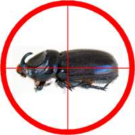
\includegraphics[width=0.75in]{static/images/crb_logo.png}\\
University of Guam Coconut Rhinoceros Beetle Biological Control Project\\
Bioassay Report generated by CRB Rearing Database v.20191027\\
https://aubreymoore.pythonanywhere.com/rearing}
\title{Bioassay Report: DUG42}
\author{Aubrey Moore and James Grasela\\University of Guam Coconut Rhinoceros Beetle Biocontrol Project}
\begin{document}
\begin{titlepage}
    \maketitle
    \tableofcontents
\end{titlepage}

\clearpage
\section{Summary}
\section{Description}
Adult beetles incubated at 30{\celsius} and 80\% RH for more than 2 weeks to observe possible contamination from green muscardine fungus infection were employed in a bioassay to determine the susceptibility of adults to infection by a virus isolate collected from the Philippines (\textbf{Dug42}). Treatment 1 consisted of 10-20 {\micro}l sterile filtered water injected at a point on the ventral surface at the junction of the hind leg and the thoracic using a sterile needle. Treatment 2 consisted of 10-20 {\micro}l heat-inactivated virus injection while in the treatment 3, beetles were injected with 10-20 {\micro}l of untreated virus preparation.  Adults were then placed in clean glass mason jars (bleach-treated) with a piece of banana added for food. Beetles were incubated at 30{\celsius} and 80\% RH in a Percival incubator. All beetles were weighted every other day but monitored daily for four weeks to observe any possible signs of mortality.


\subsection{Replicate 1} 

A total of 10 adult females and five adult males distributed among the three treatments were employed in this replicate. 

\subsection{Replicate 2}

A total of seven adult females and eight adult males distributed among the three treatments were employed in this replicate.

\clearpage
\section{Mortality}

\begin{tabular}{llrrrrr}
\toprule
{} & bioassay\_treatment &  ntotal &  ndead &  mortality &  adjusted\_mortality &  significance \\
\midrule
0 &            control &      10 &      5 &        0.5 &                 0.0 &      1.000000 \\
1 &   heat inactivated &      10 &      7 &        0.7 &                 0.4 &      0.649917 \\
2 &              virus &      10 &      7 &        0.7 &                 0.4 &      0.649917 \\
\bottomrule
\end{tabular}


\begin{center}
     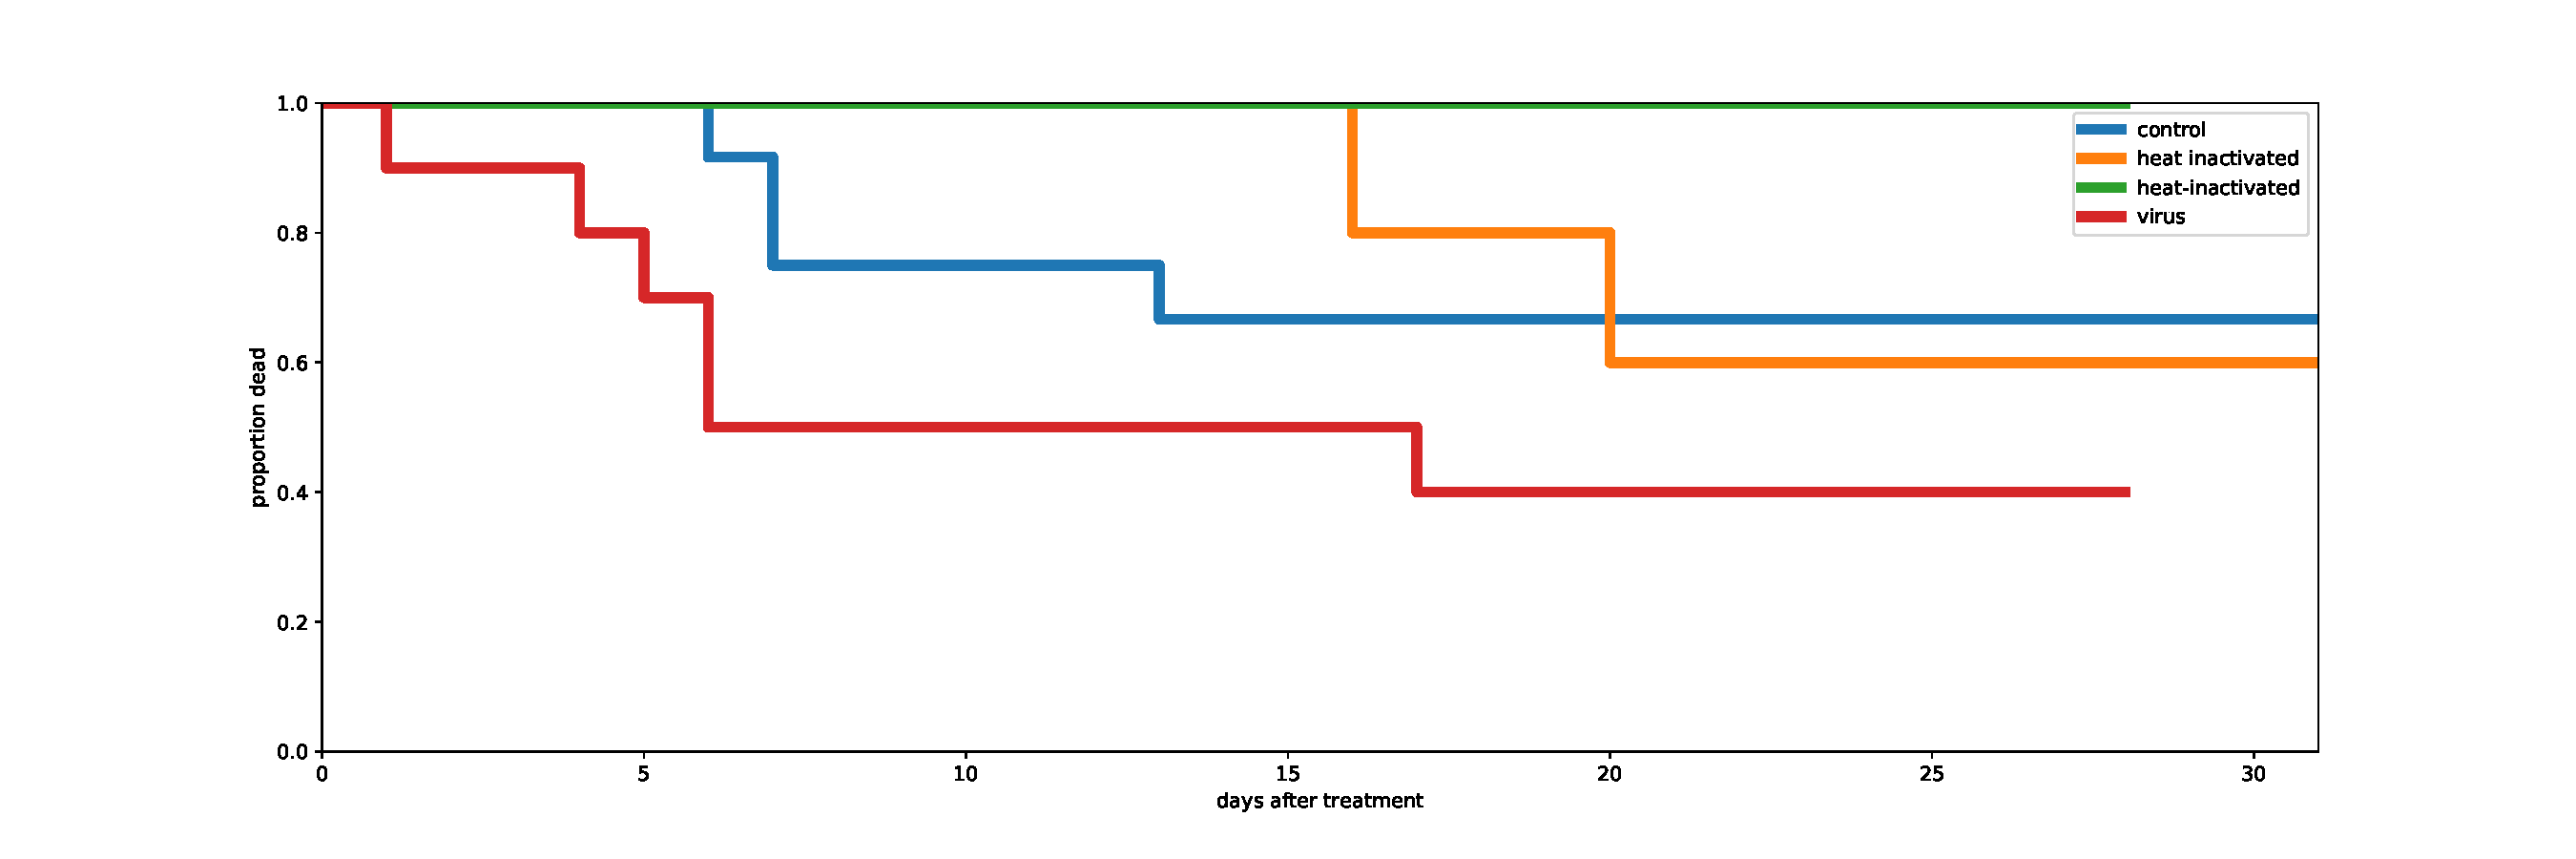
\includegraphics[width=\textwidth]{survivorshipfig.pdf}
\end{center}



    \begin{table}[h!]
    \centering
    \caption{Pairwise differences among mortality curves.}
\begin{tabular}{llrr}
\toprule
                 &       &  test\_statistic &         p \\
\midrule
control & heat inactivated &        1.920677 &  0.165782 \\
                 & virus &        2.020872 &  0.155150 \\
heat inactivated & virus &        0.007094 &  0.932879 \\
\bottomrule
\end{tabular}
\end{table} 

\clearpage
\section{Change in Mass}
Change in mass section goes here.

\begin{center}
     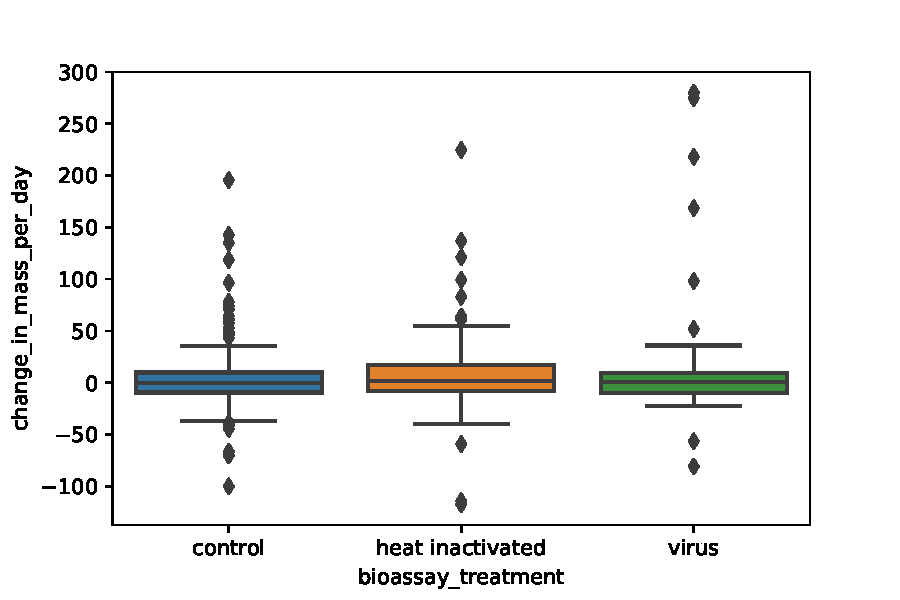
\includegraphics[width=\textwidth]{bp.pdf}
\end{center}

\begin{tabular}{lrrr}
\toprule
{} &   control &  heat inactivated &  virus \\
\midrule
control          & -1.000000 &          0.901325 &    1.0 \\
heat inactivated &  0.901325 &         -1.000000 &    1.0 \\
virus            &  1.000000 &          1.000000 &   -1.0 \\
\bottomrule
\end{tabular}


\clearpage
\section{Post Mortem Images}
\subsection{control}

\begin{figure}[h!]
    \centering
    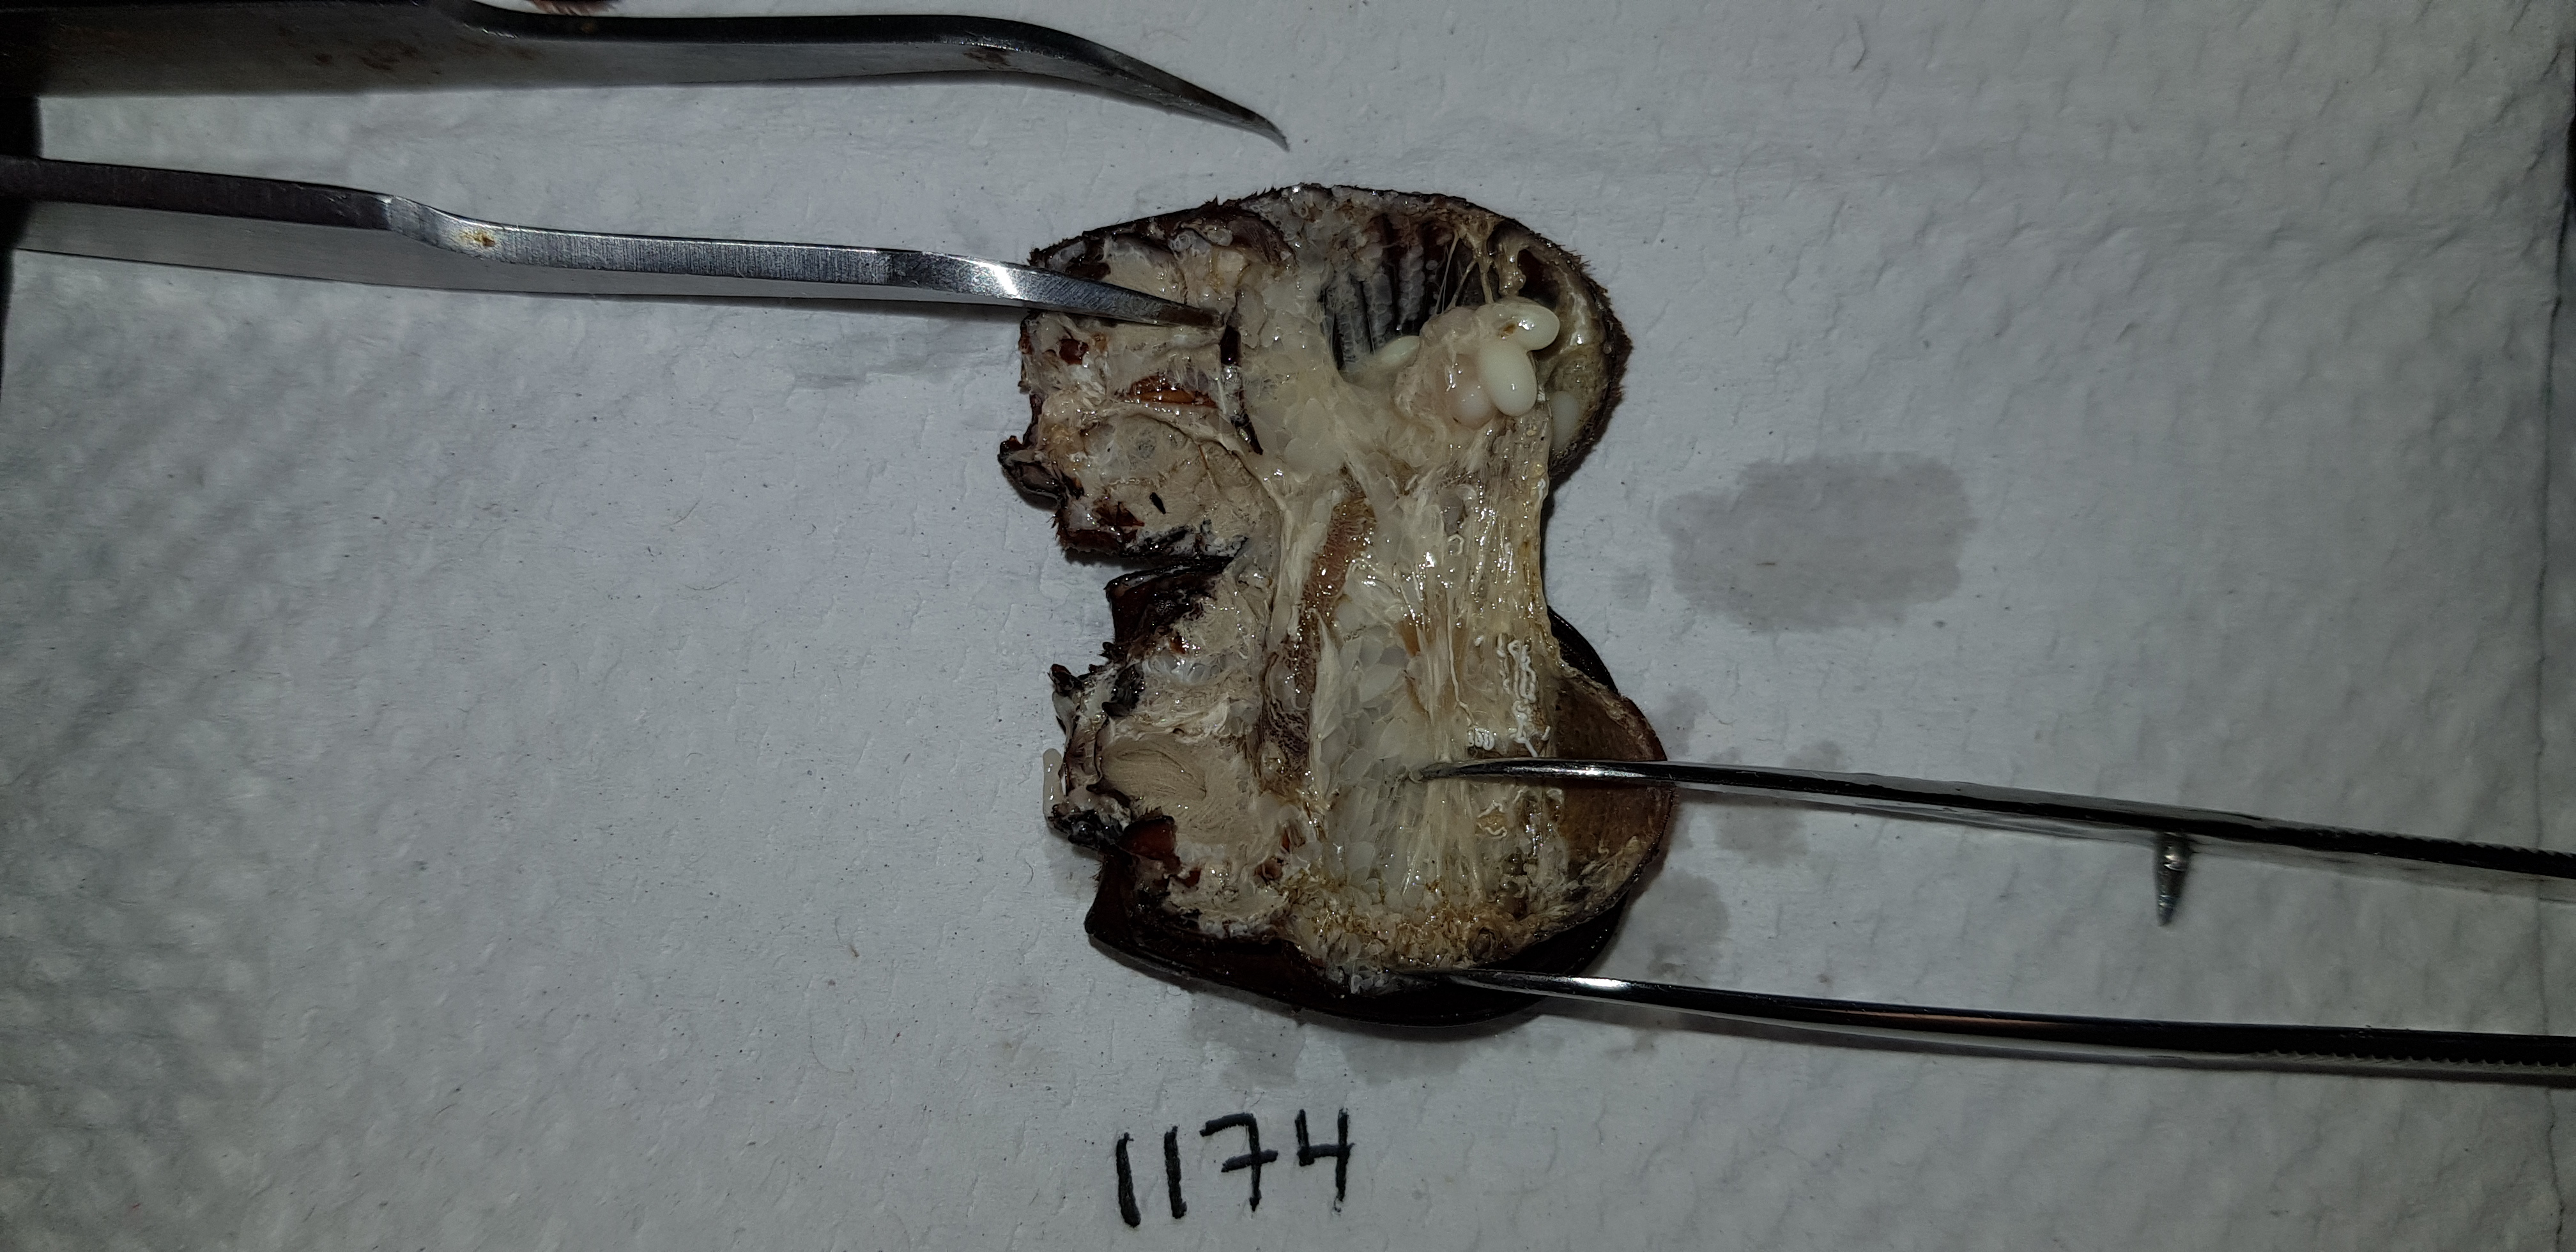
\includegraphics[width=\linewidth, height=\textheight, keepaspectratio]{uploads/btl.pm_image.925167688fe01c89.447567343220313137345f5265702d3120636f6e74726f6c2e6a7067.jpg}
    \caption{Bioassay: DUG42-1; Treatment: control; Beetle ID: 46}
\end{figure}
\clearpage

\begin{figure}[h!]
    \centering
    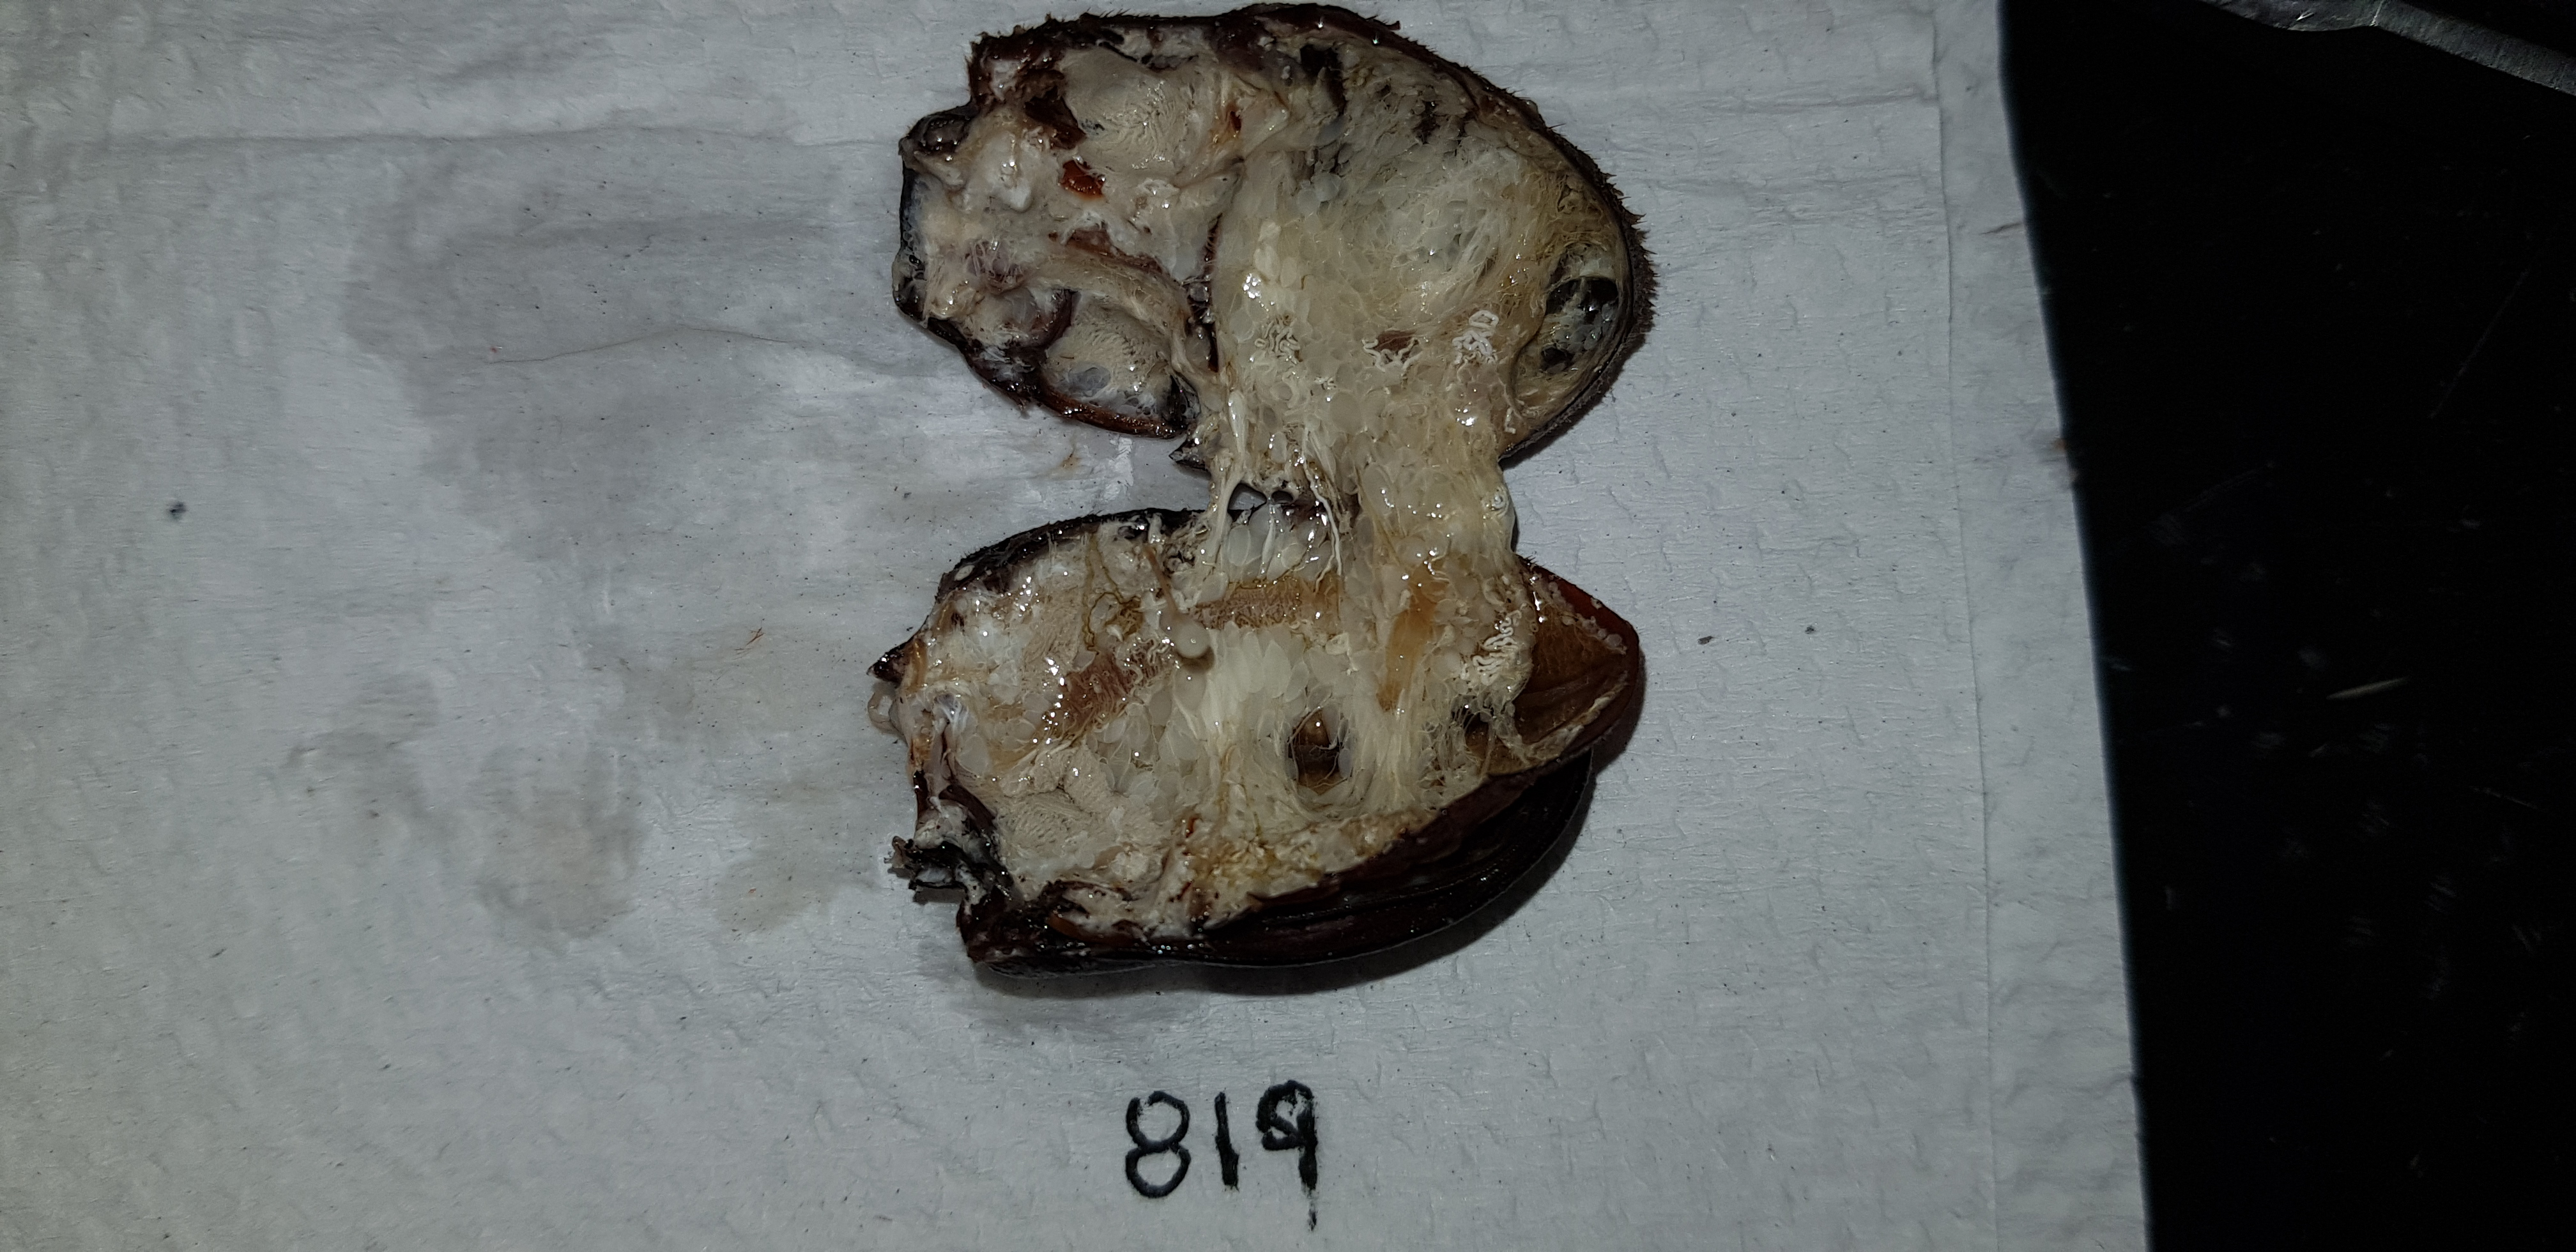
\includegraphics[width=\linewidth, height=\textheight, keepaspectratio]{uploads/btl.pm_image.bb8525578c5296ca.4475673432203831395f5265702d3120636f6e74726f6c2e6a7067.jpg}
    \caption{Bioassay: DUG42-1; Treatment: control; Beetle ID: 47}
\end{figure}
\clearpage

\begin{figure}[h!]
    \centering
    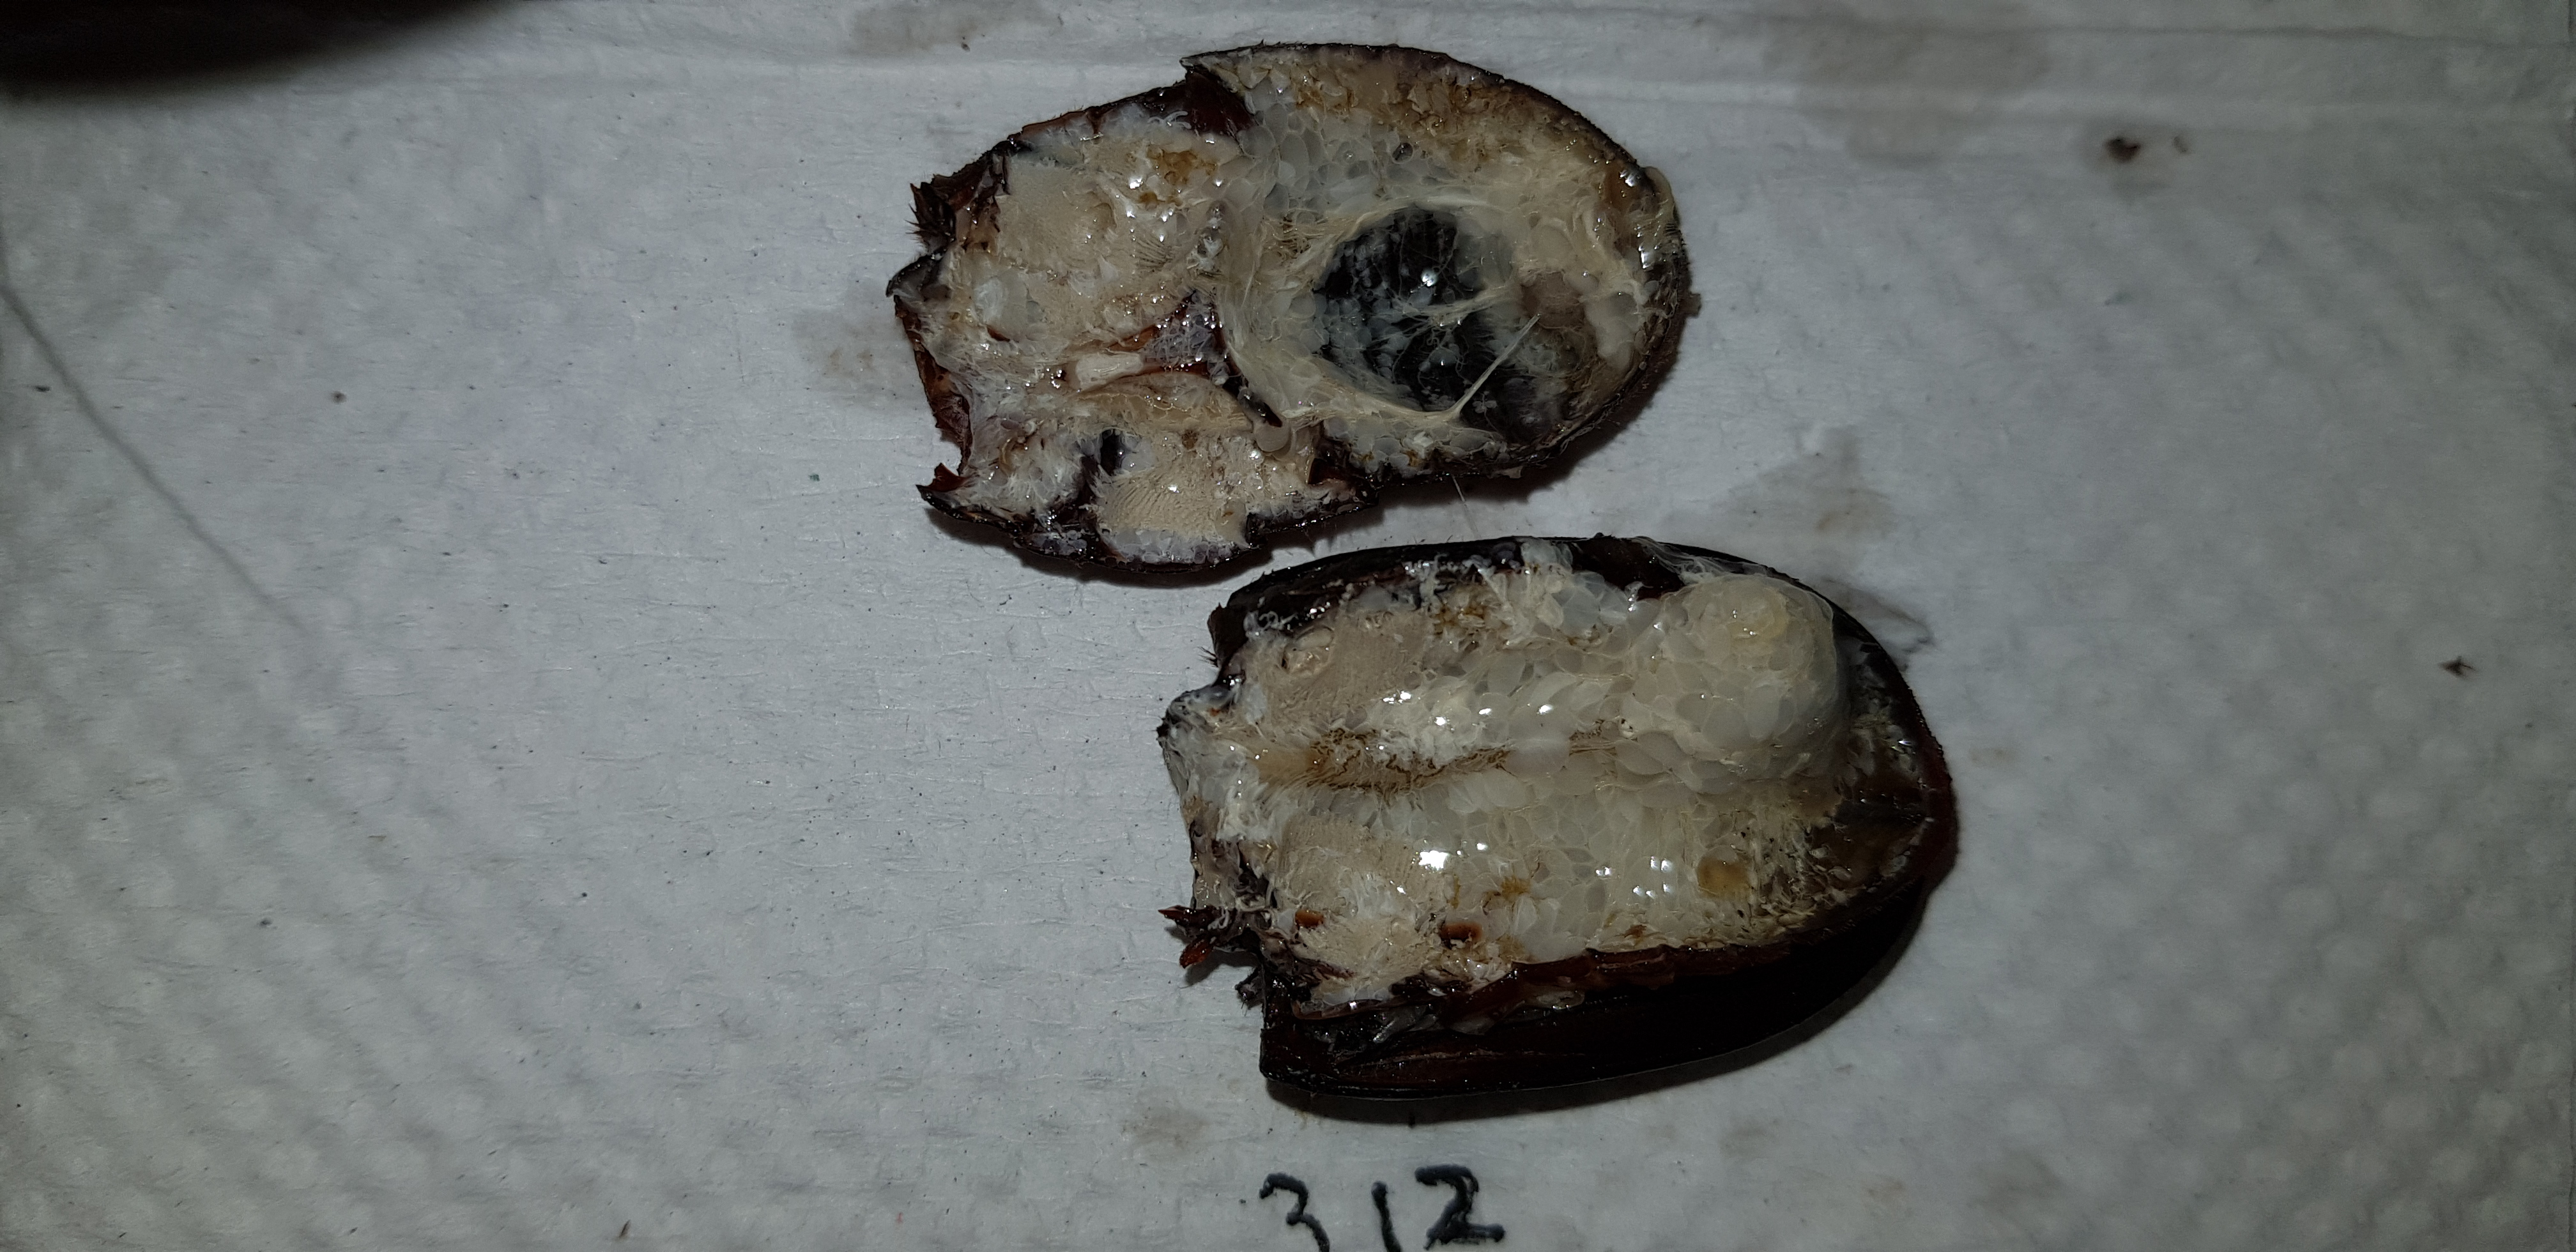
\includegraphics[width=\linewidth, height=\textheight, keepaspectratio]{uploads/btl.pm_image.8f9bf227098434cd.4475673432203331325f5265702d3120636f6e747a726f6c2e6a7067.jpg}
    \caption{Bioassay: DUG42-1; Treatment: control; Beetle ID: 48}
\end{figure}
\clearpage

\begin{figure}[h!]
    \centering
    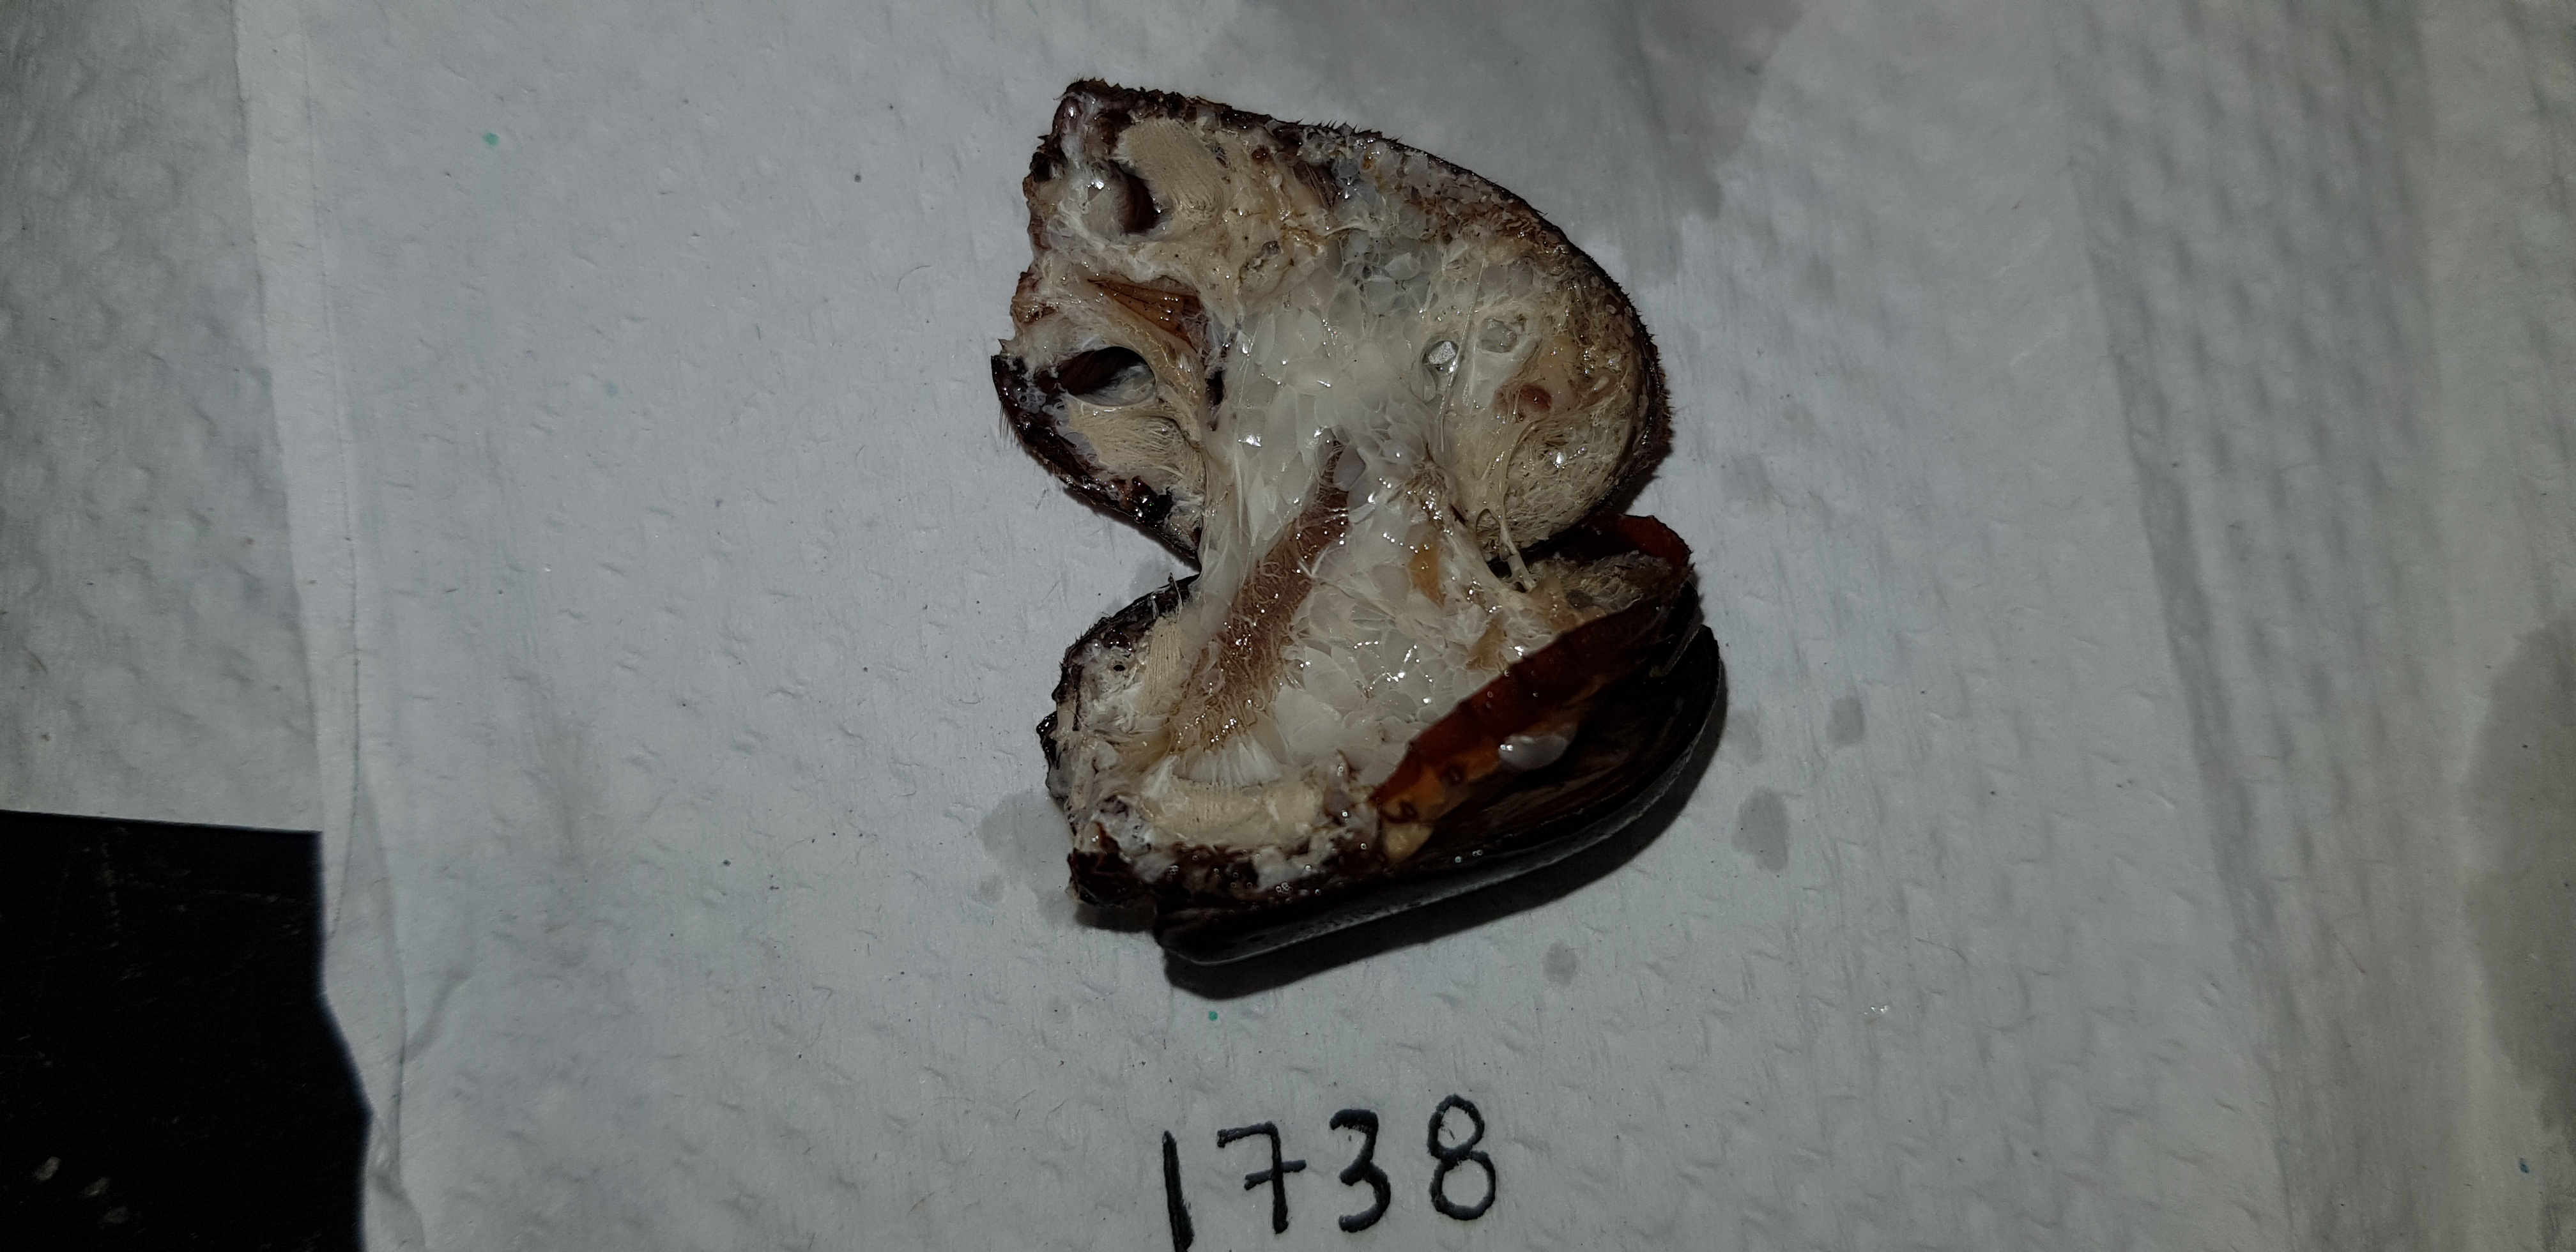
\includegraphics[width=\linewidth, height=\textheight, keepaspectratio]{uploads/btl.pm_image.b2c675174fdd2eda.447567343220313733385f5265702d3120636f6e74726f6c2e6a7067.jpg}
    \caption{Bioassay: DUG42-1; Treatment: control; Beetle ID: 49}
\end{figure}
\clearpage

\begin{figure}[h!]
    \centering
    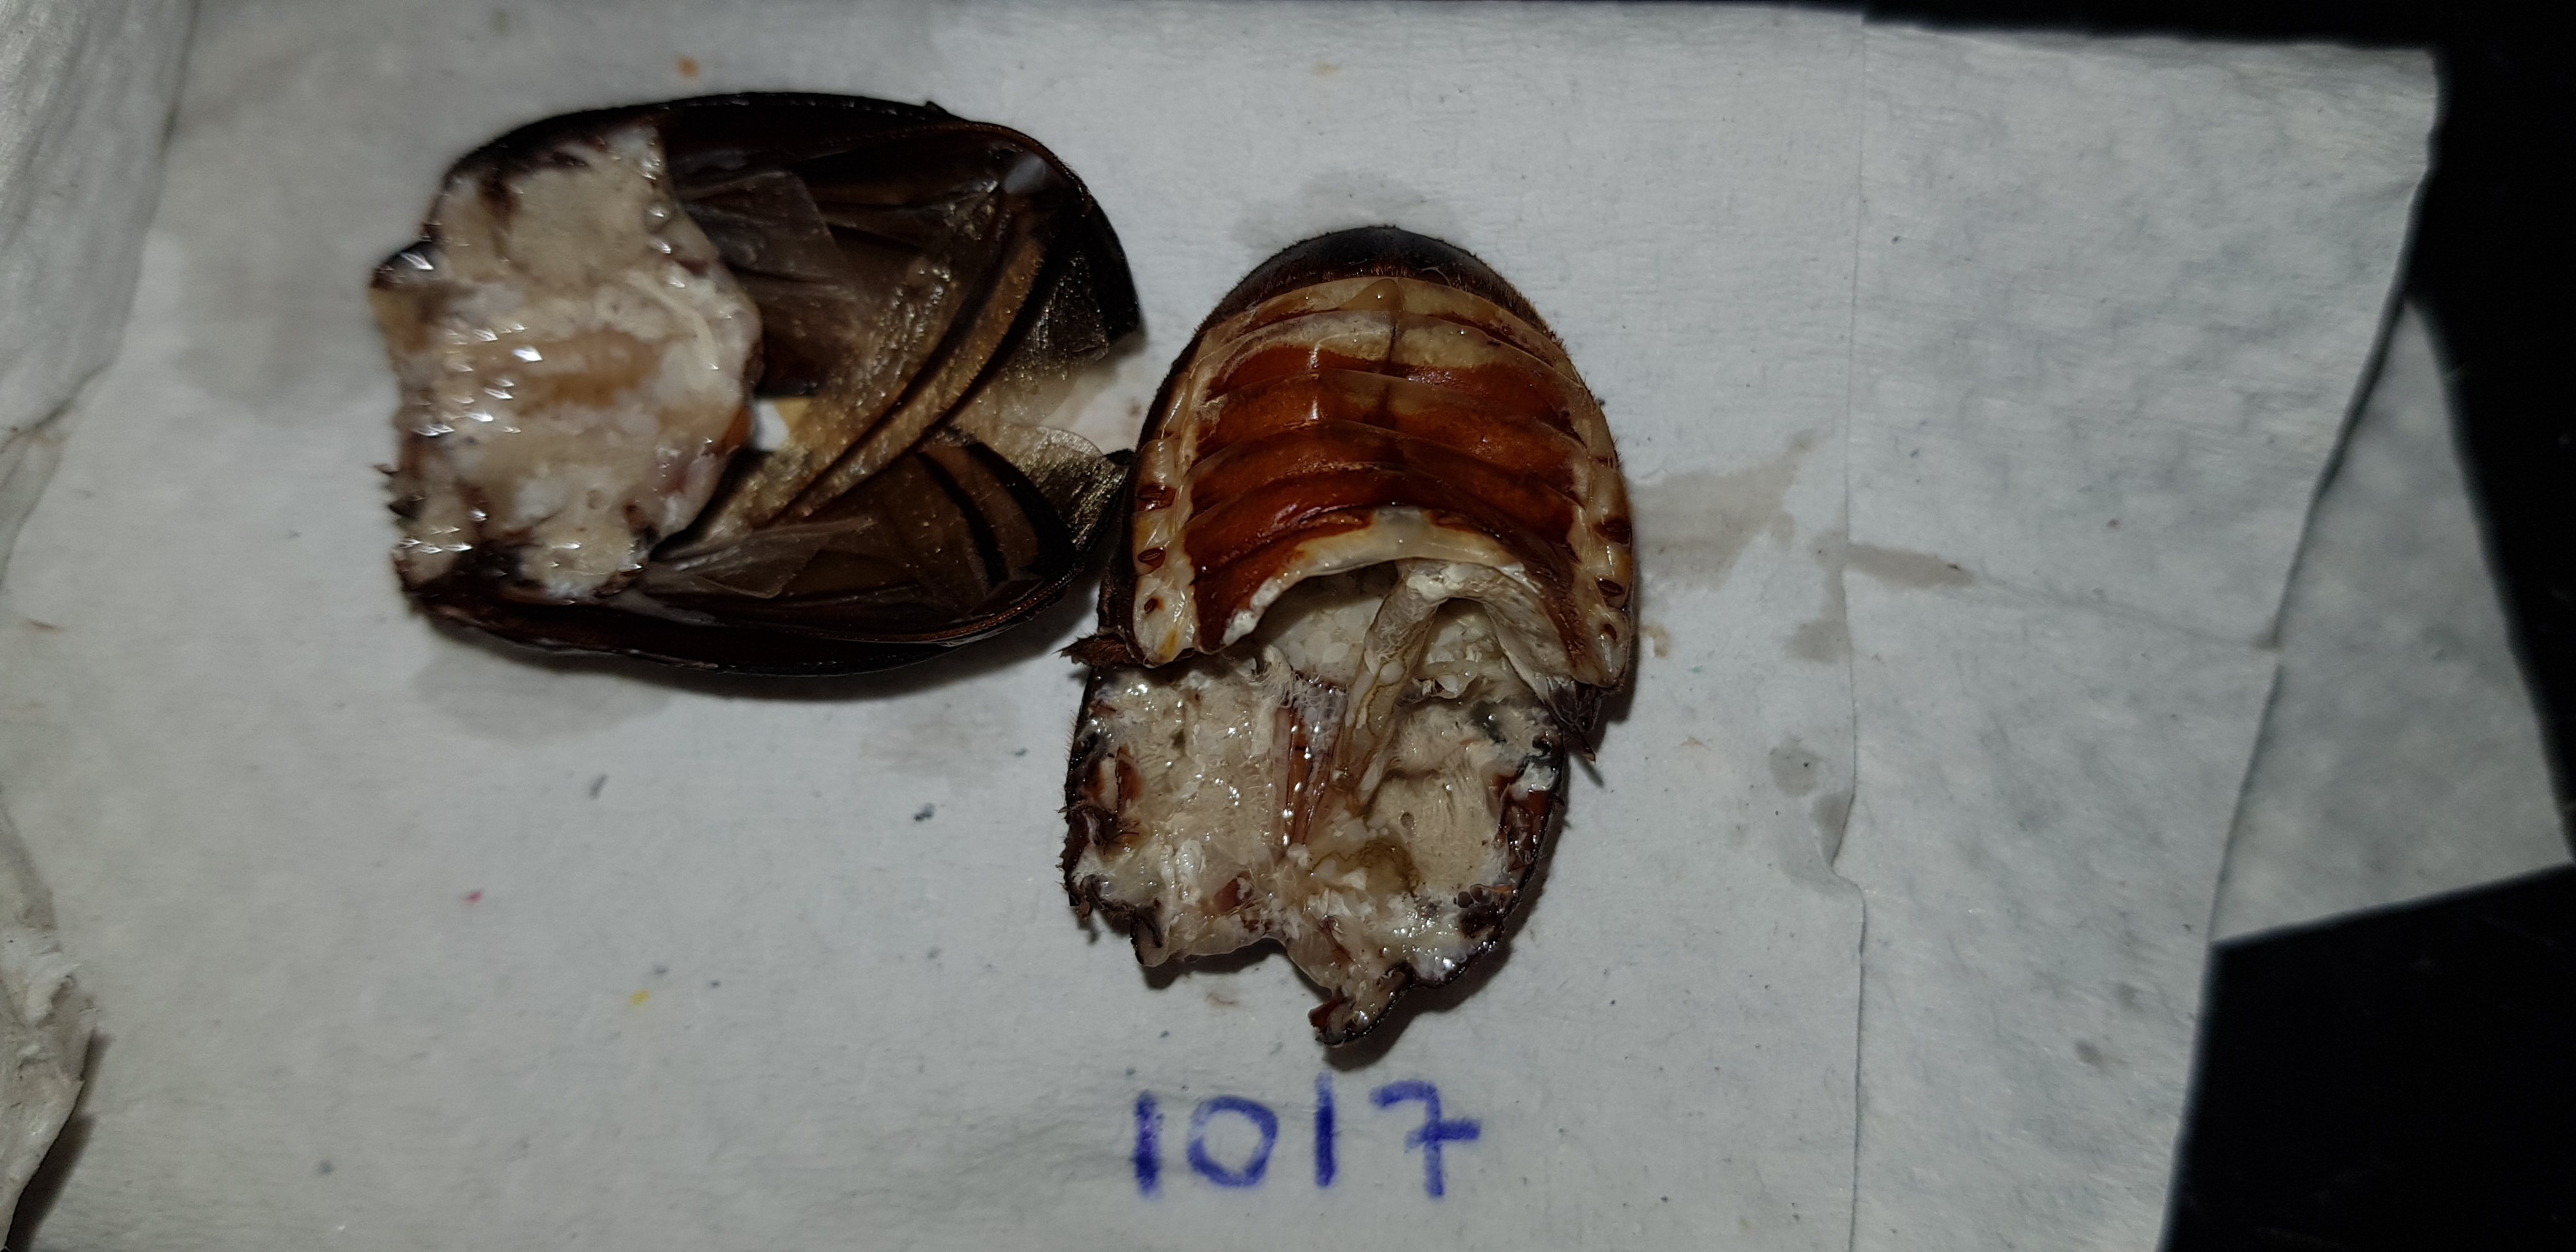
\includegraphics[width=\linewidth, height=\textheight, keepaspectratio]{uploads/btl.pm_image.950cdb8728985088.447567343220313031375f5265702d3120636f6e74726f6c2e6a7067.jpg}
    \caption{Bioassay: DUG42-1; Treatment: control; Beetle ID: 50}
\end{figure}
\clearpage

\begin{figure}[h!]
    \centering
    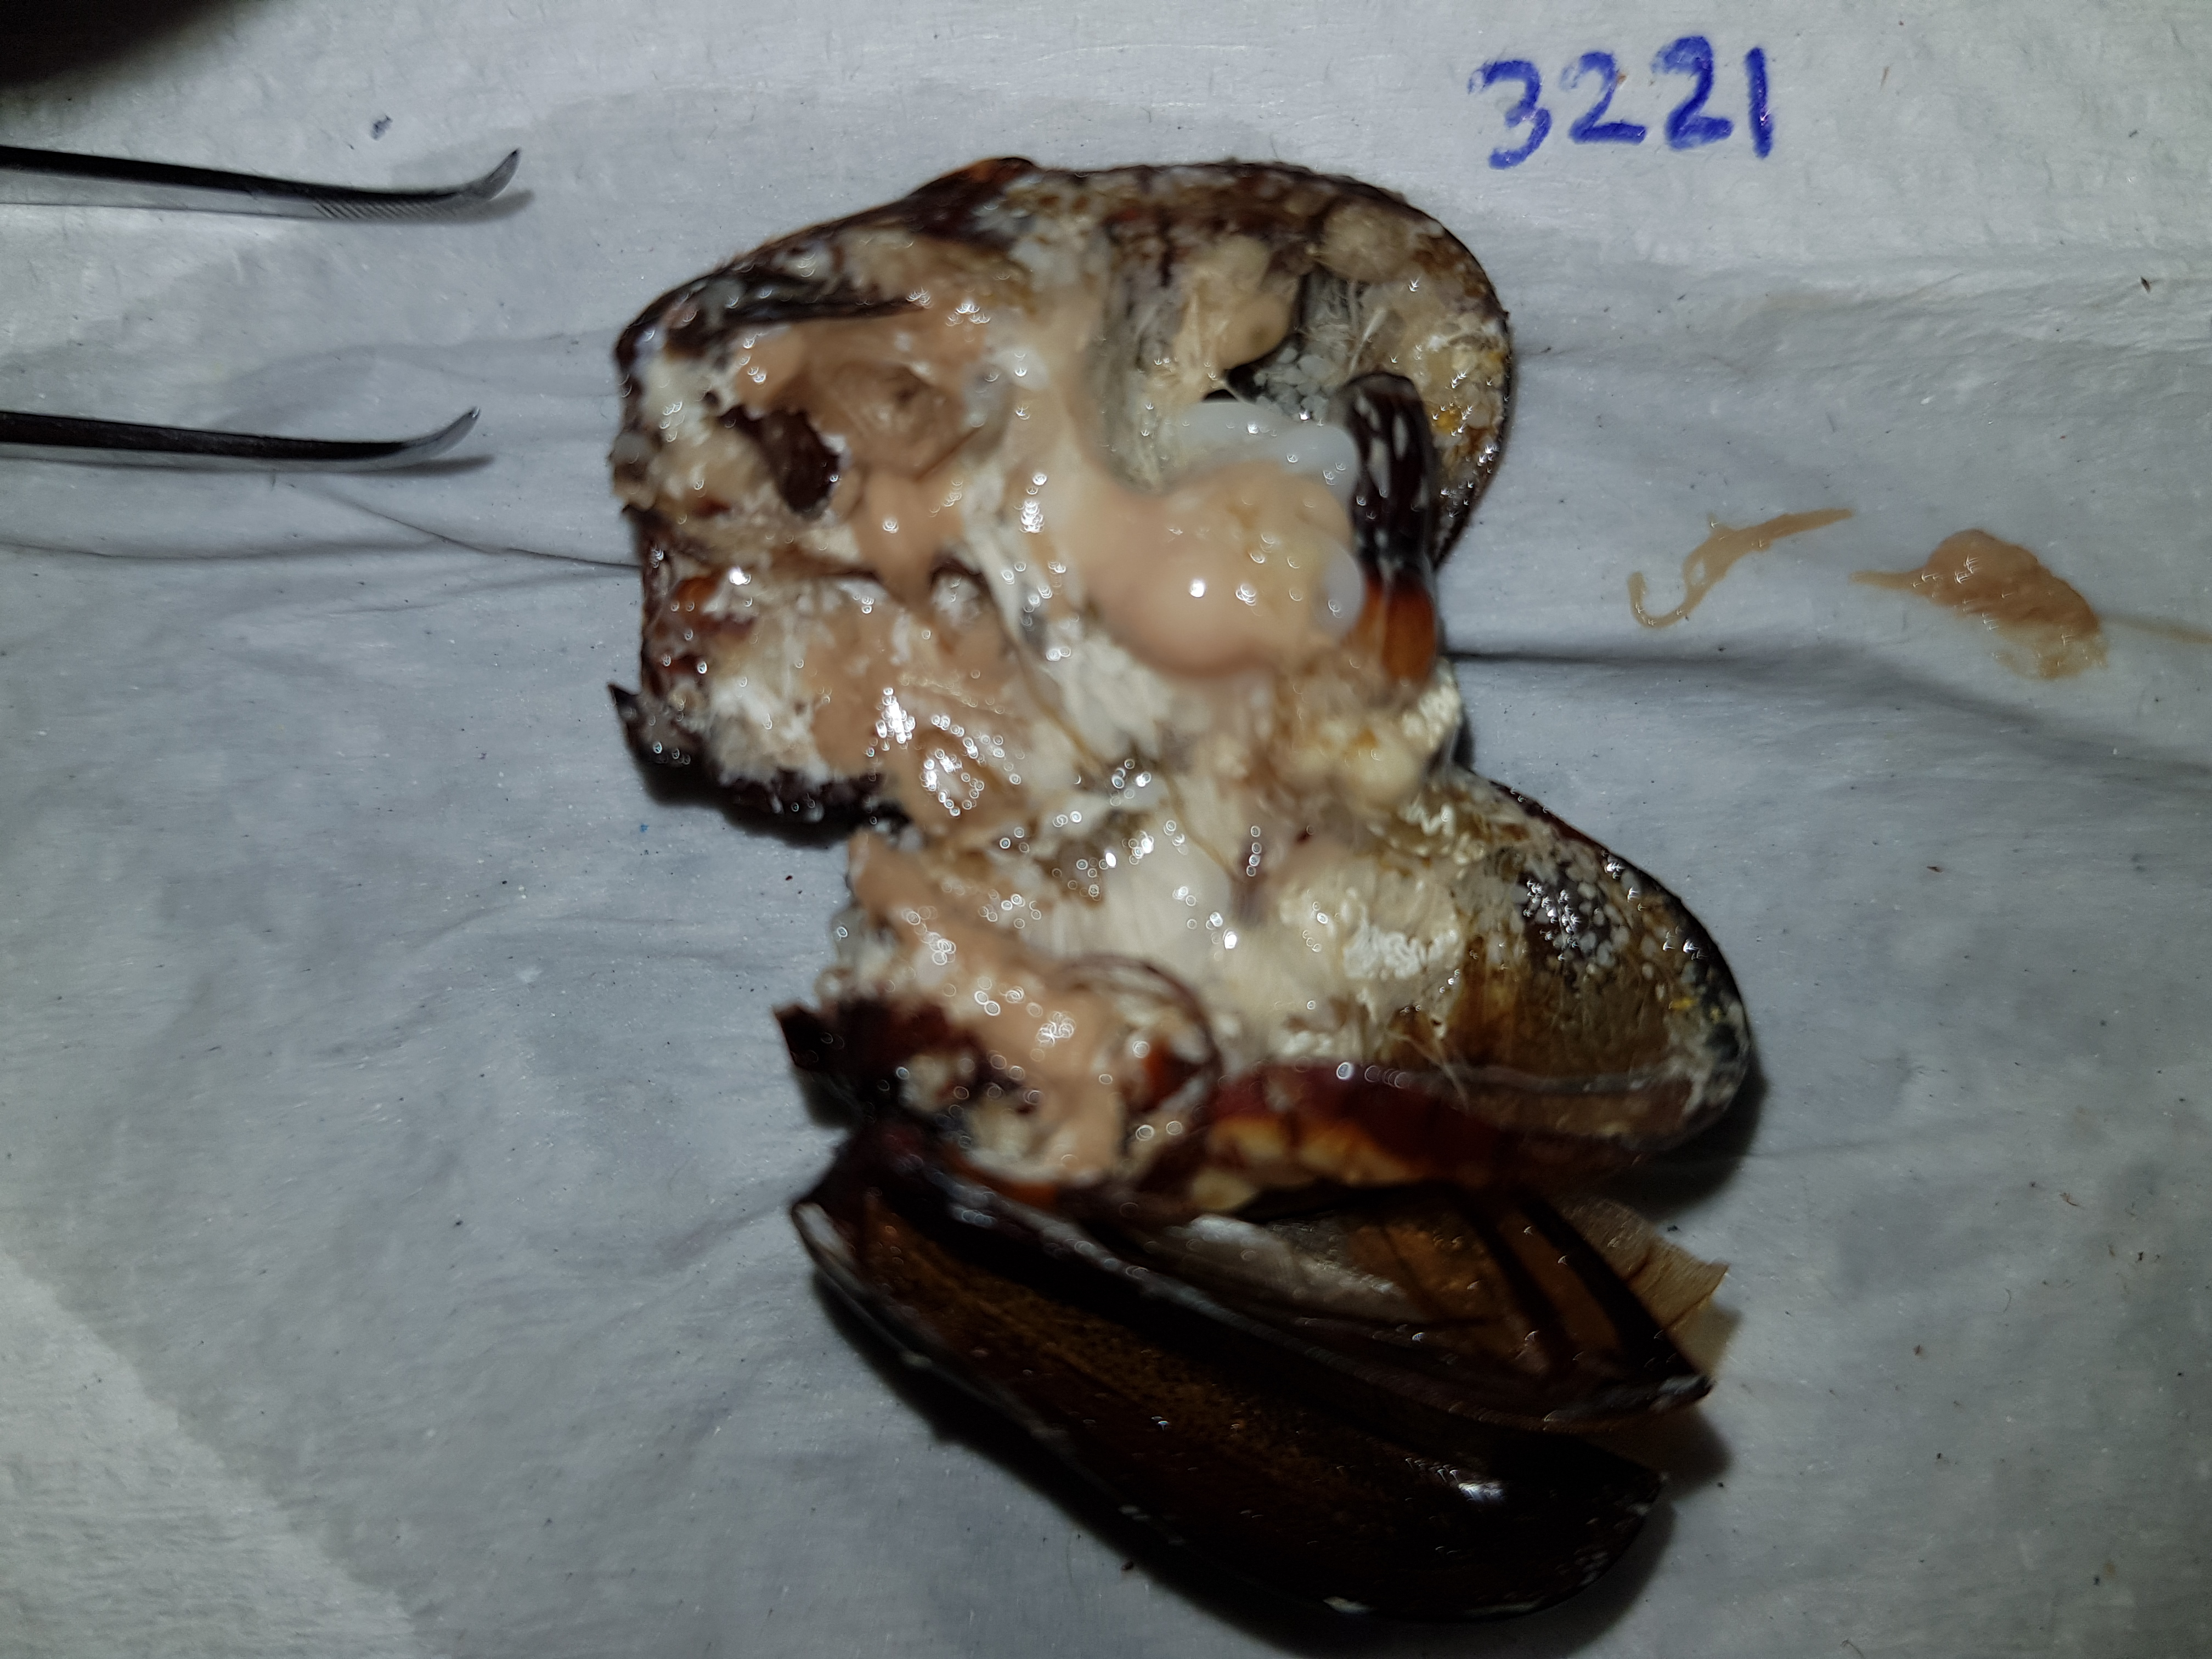
\includegraphics[width=\linewidth, height=\textheight, keepaspectratio]{uploads/btl.pm_image.a6e6336e68e00d61.447567343220333232315f5265702d3220636f6e74726f6c2e6a7067.jpg}
    \caption{Bioassay: DUG42-2; Treatment: control; Beetle ID: 61}
\end{figure}
\clearpage

\begin{figure}[h!]
    \centering
    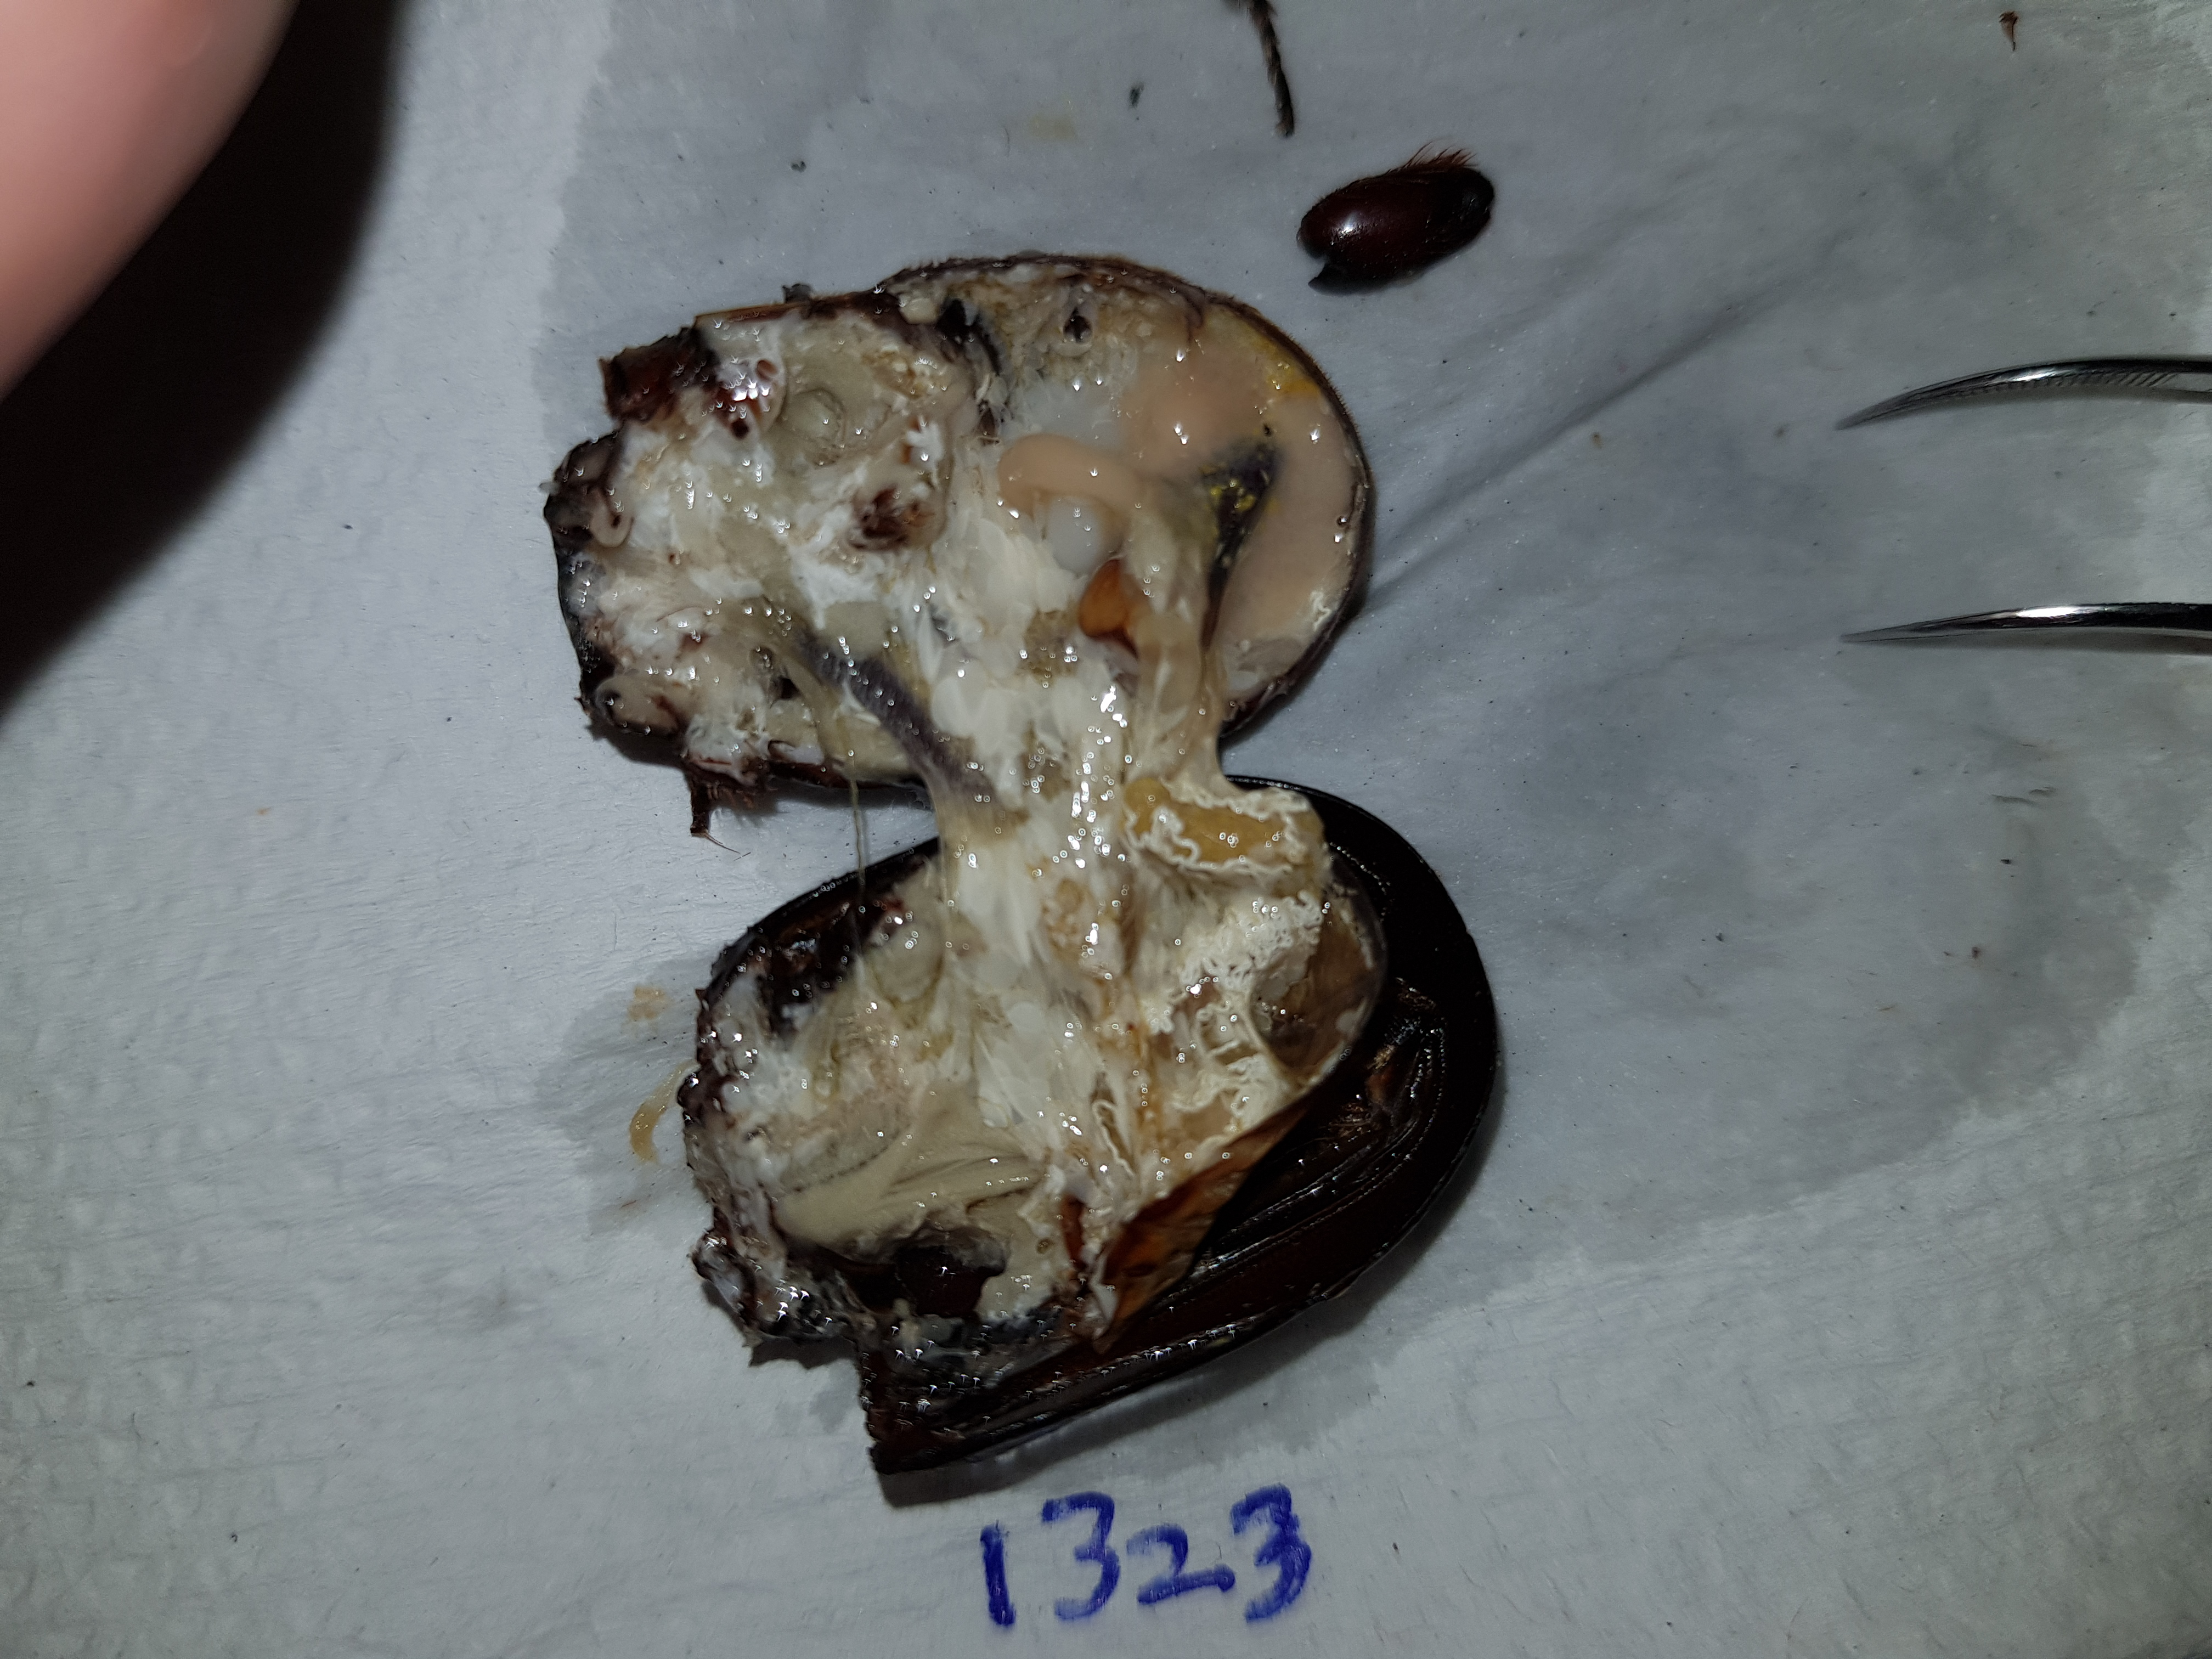
\includegraphics[width=\linewidth, height=\textheight, keepaspectratio]{uploads/btl.pm_image.adc7457e72c06e1f.447567343220313332335f5265702d3220636f6e74726f6c2e6a7067.jpg}
    \caption{Bioassay: DUG42-2; Treatment: control; Beetle ID: 62}
\end{figure}
\clearpage

\begin{figure}[h!]
    \centering
    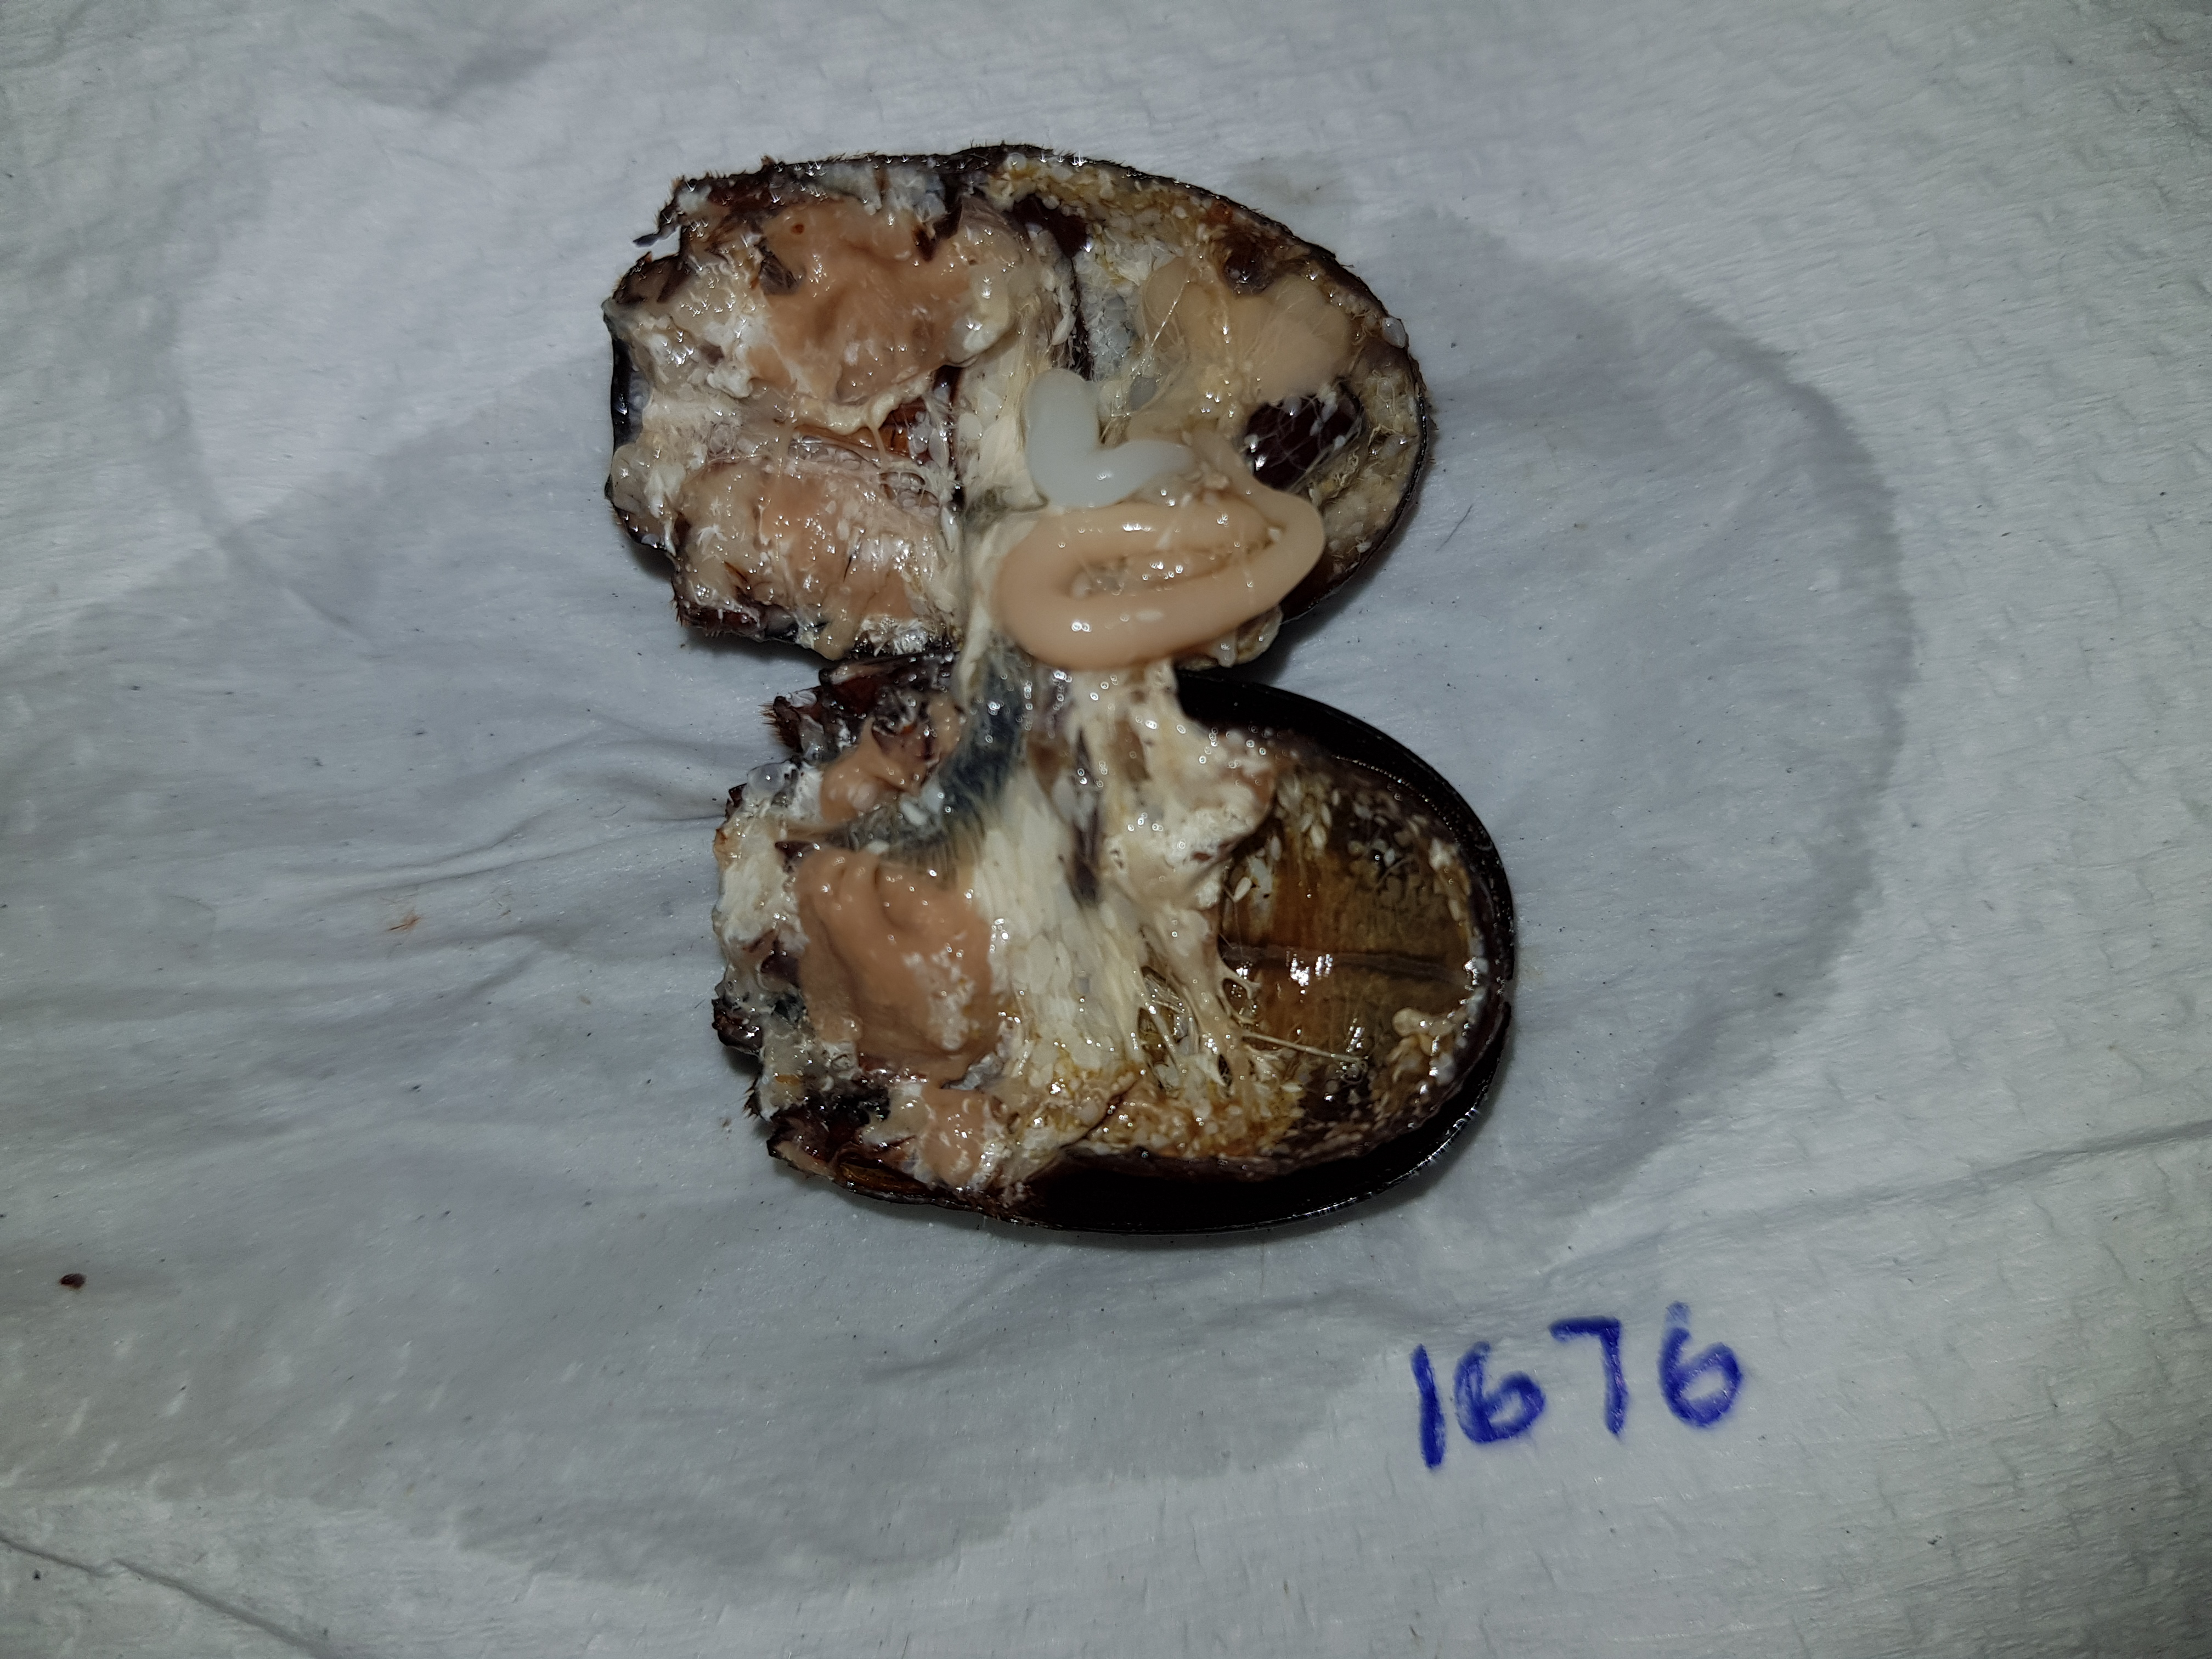
\includegraphics[width=\linewidth, height=\textheight, keepaspectratio]{uploads/btl.pm_image.aa4294f1fcd4bfab.447567343220313637365f5265702d322020636f6e74726f6c2e6a7067.jpg}
    \caption{Bioassay: DUG42-2; Treatment: control; Beetle ID: 63}
\end{figure}
\clearpage

\begin{figure}[h!]
    \centering
    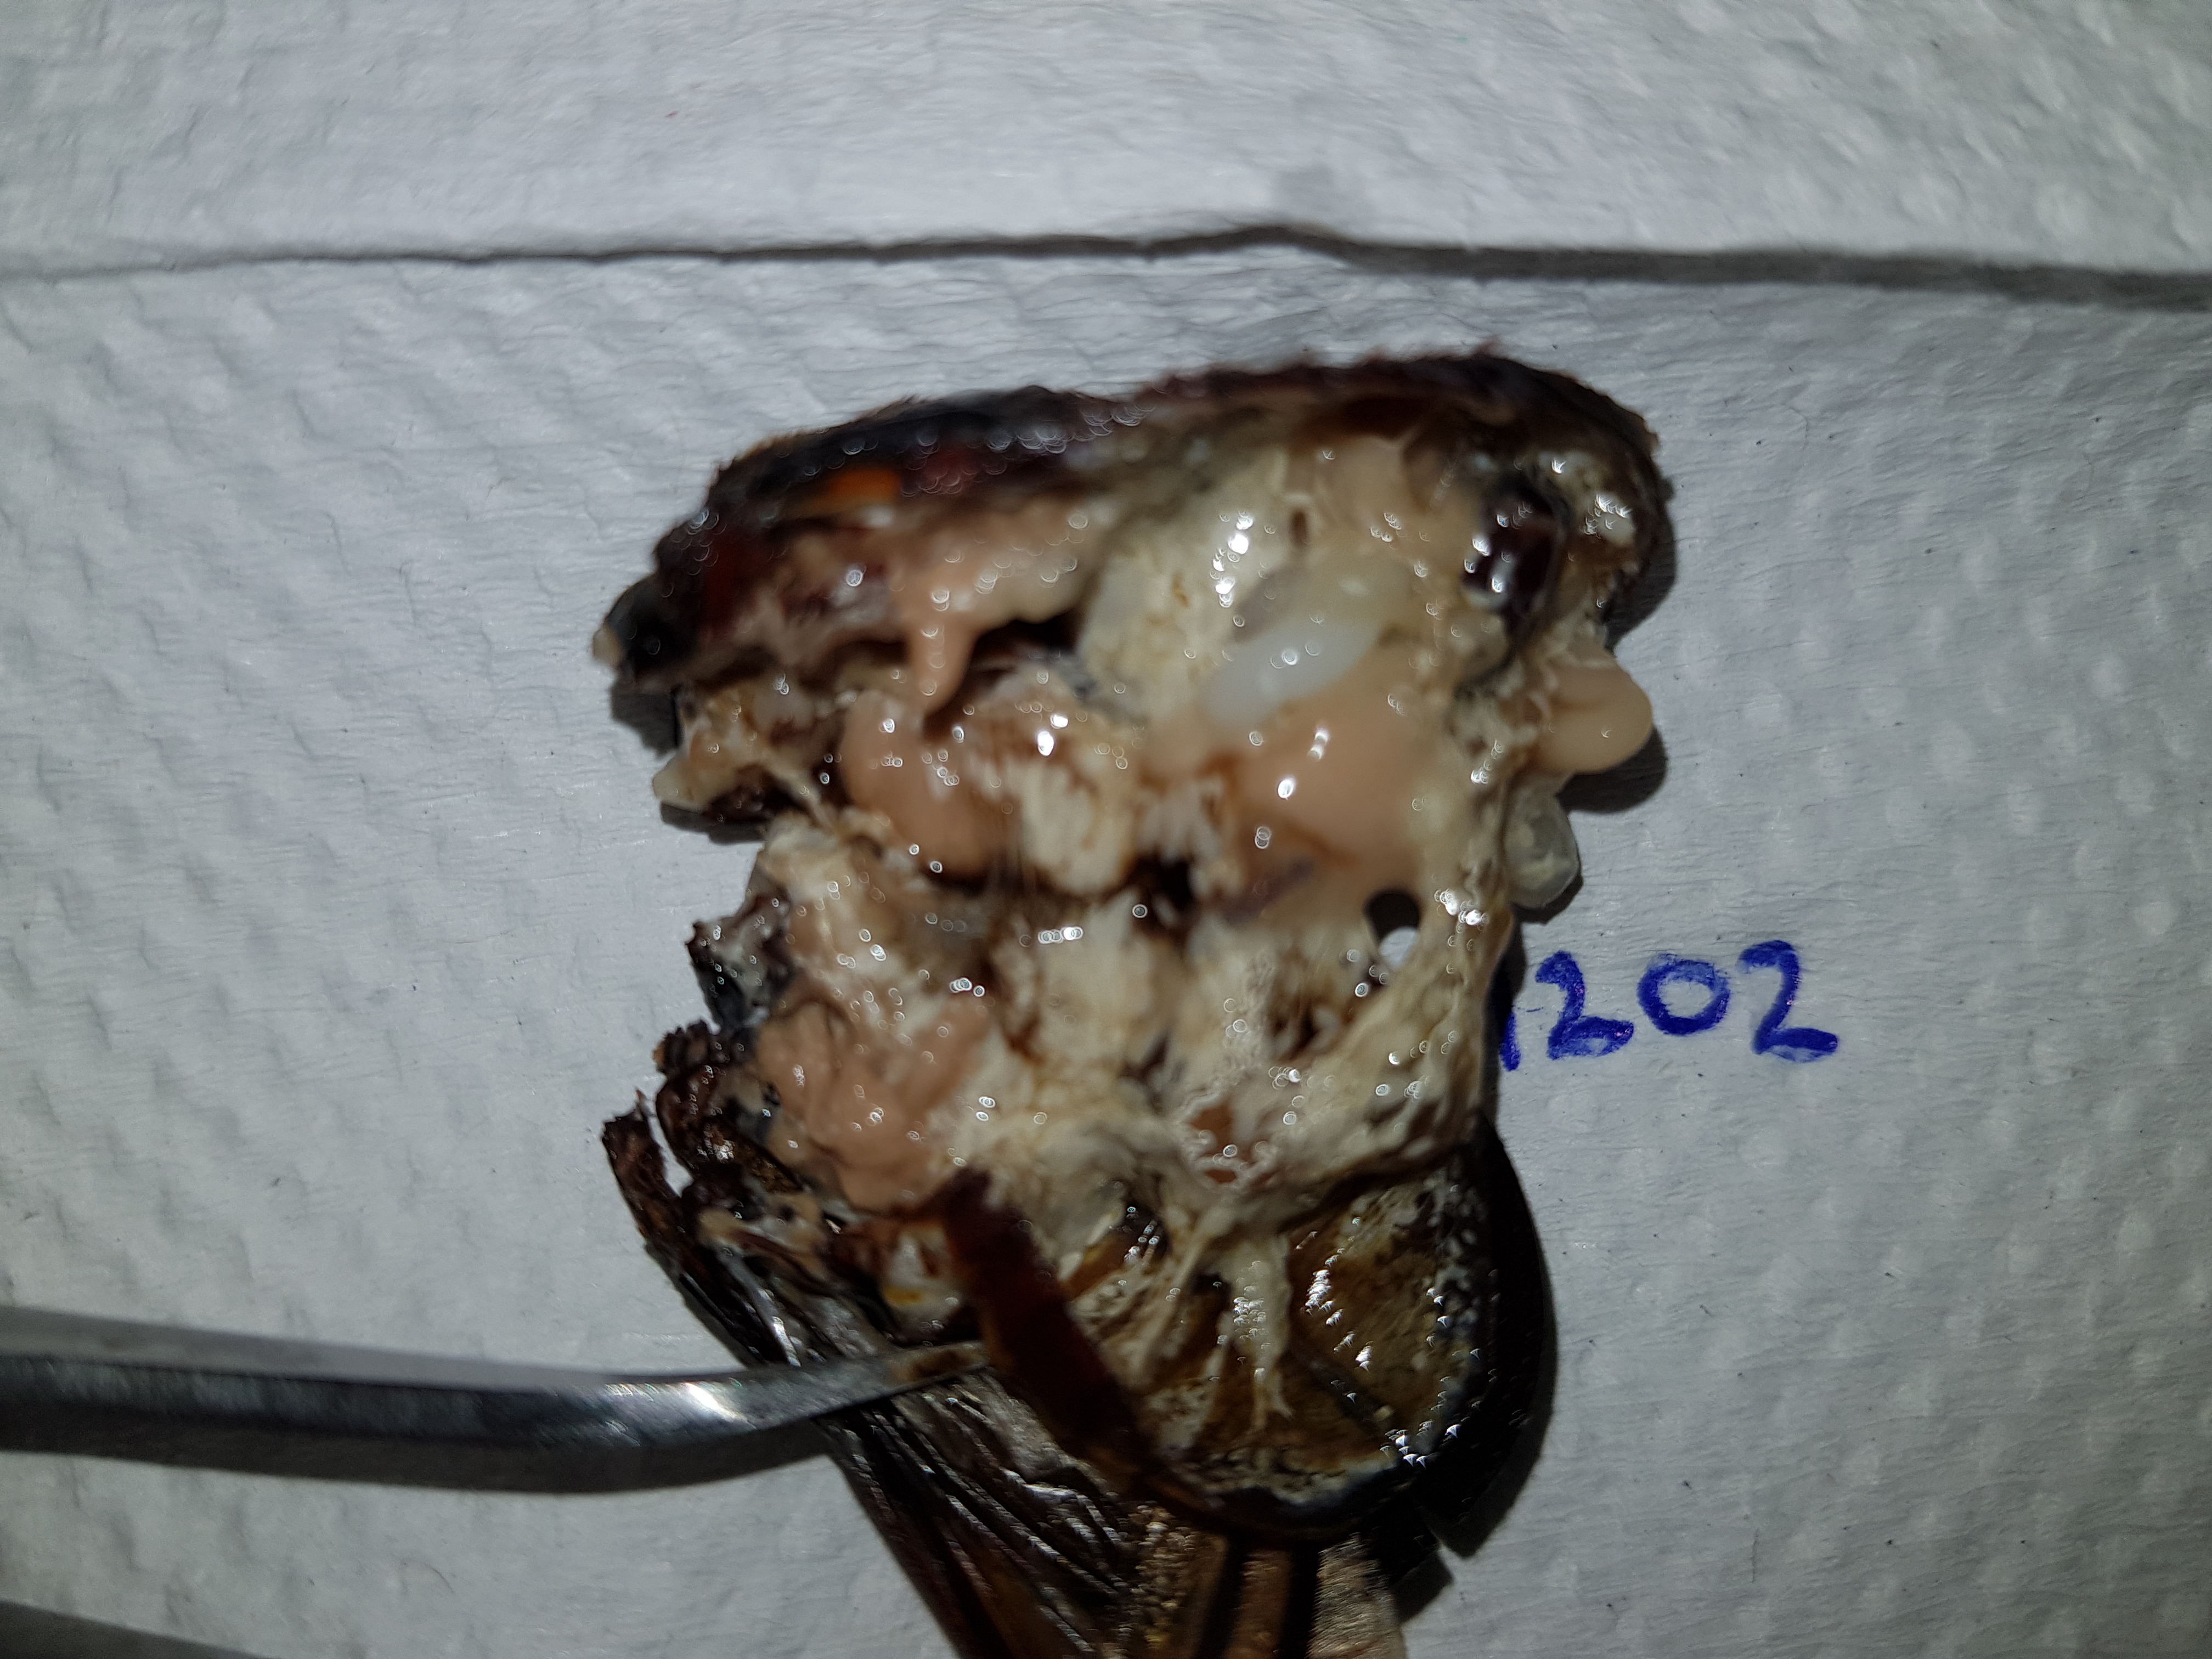
\includegraphics[width=\linewidth, height=\textheight, keepaspectratio]{uploads/btl.pm_image.9ac50522aea10415.447567343220313230325f5265702d3220636f6e74726f6c2e6a7067.jpg}
    \caption{Bioassay: DUG42-2; Treatment: control; Beetle ID: 64}
\end{figure}
\clearpage

\begin{figure}[h!]
    \centering
    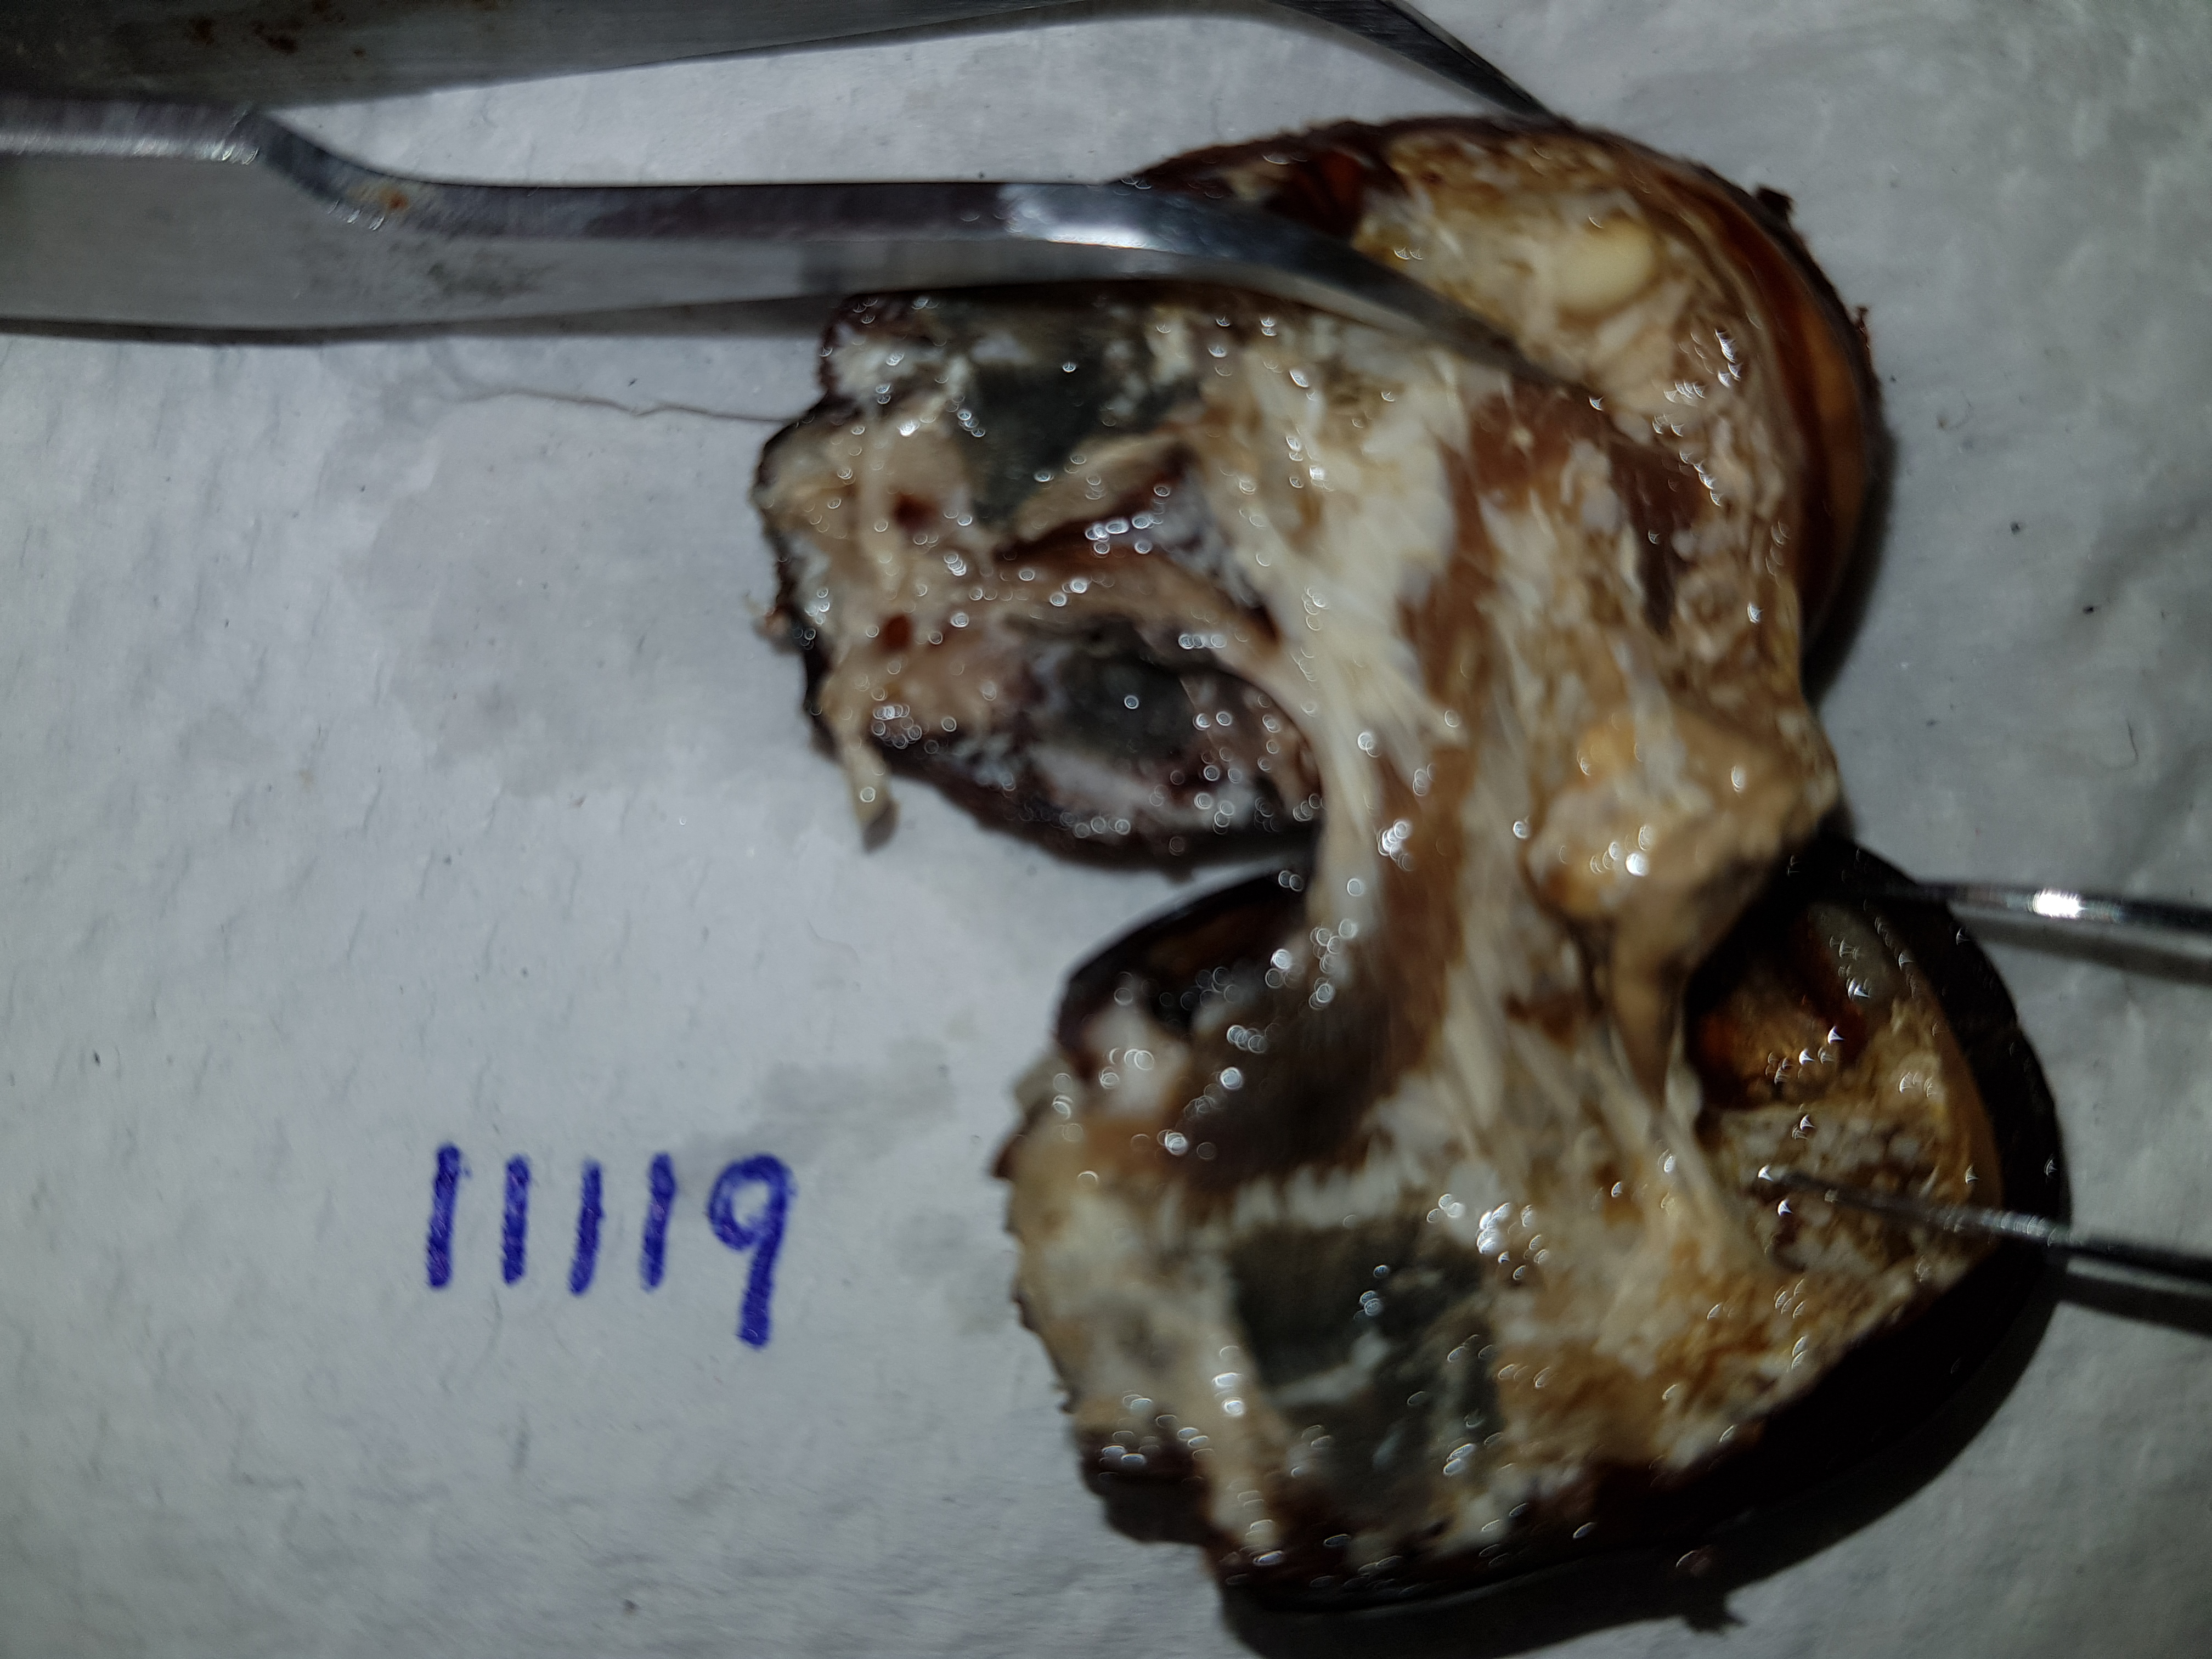
\includegraphics[width=\linewidth, height=\textheight, keepaspectratio]{uploads/btl.pm_image.9c977e79c5d4ef97.44756734322031313131395f5265702d3220636f6e74726f6c2e6a7067.jpg}
    \caption{Bioassay: DUG42-2; Treatment: control; Beetle ID: 65}
\end{figure}
\clearpage

\subsection{heat inactivated}

\begin{figure}[h!]
    \centering
    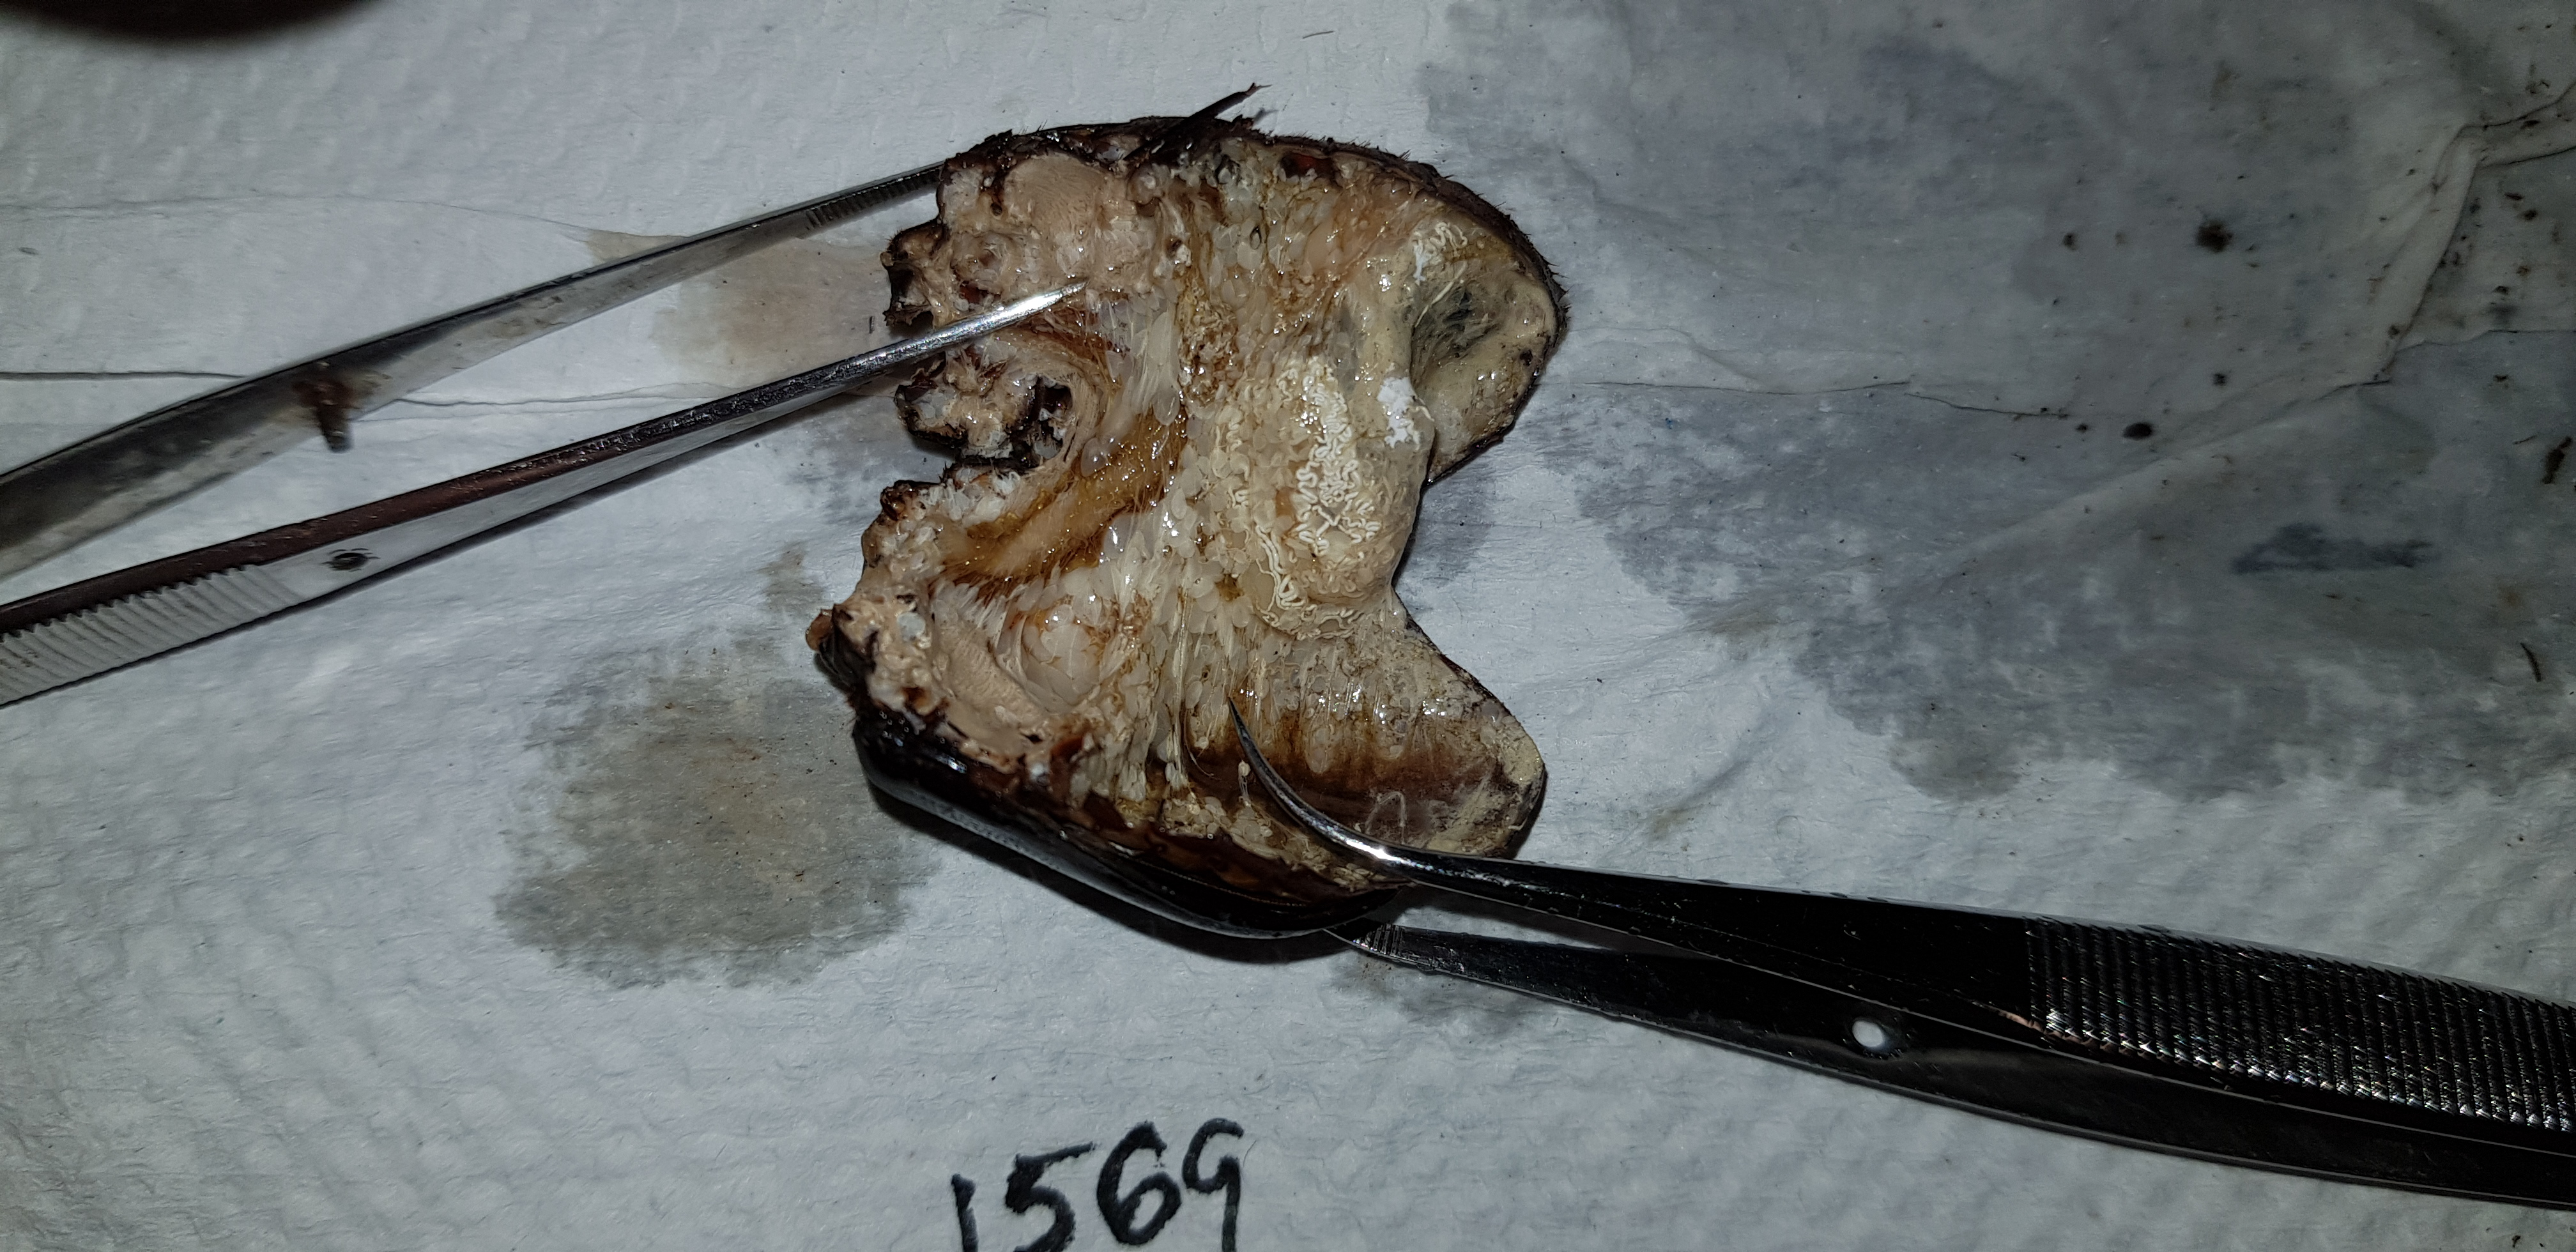
\includegraphics[width=\linewidth, height=\textheight, keepaspectratio]{uploads/btl.pm_image.bcf926e3e475d507.447567343220313536395f5265702d3120636f6e74726f6c2e6a7067.jpg}
    \caption{Bioassay: DUG42-1; Treatment: heat inactivated; Beetle ID: 51}
\end{figure}
\clearpage

\begin{figure}[h!]
    \centering
    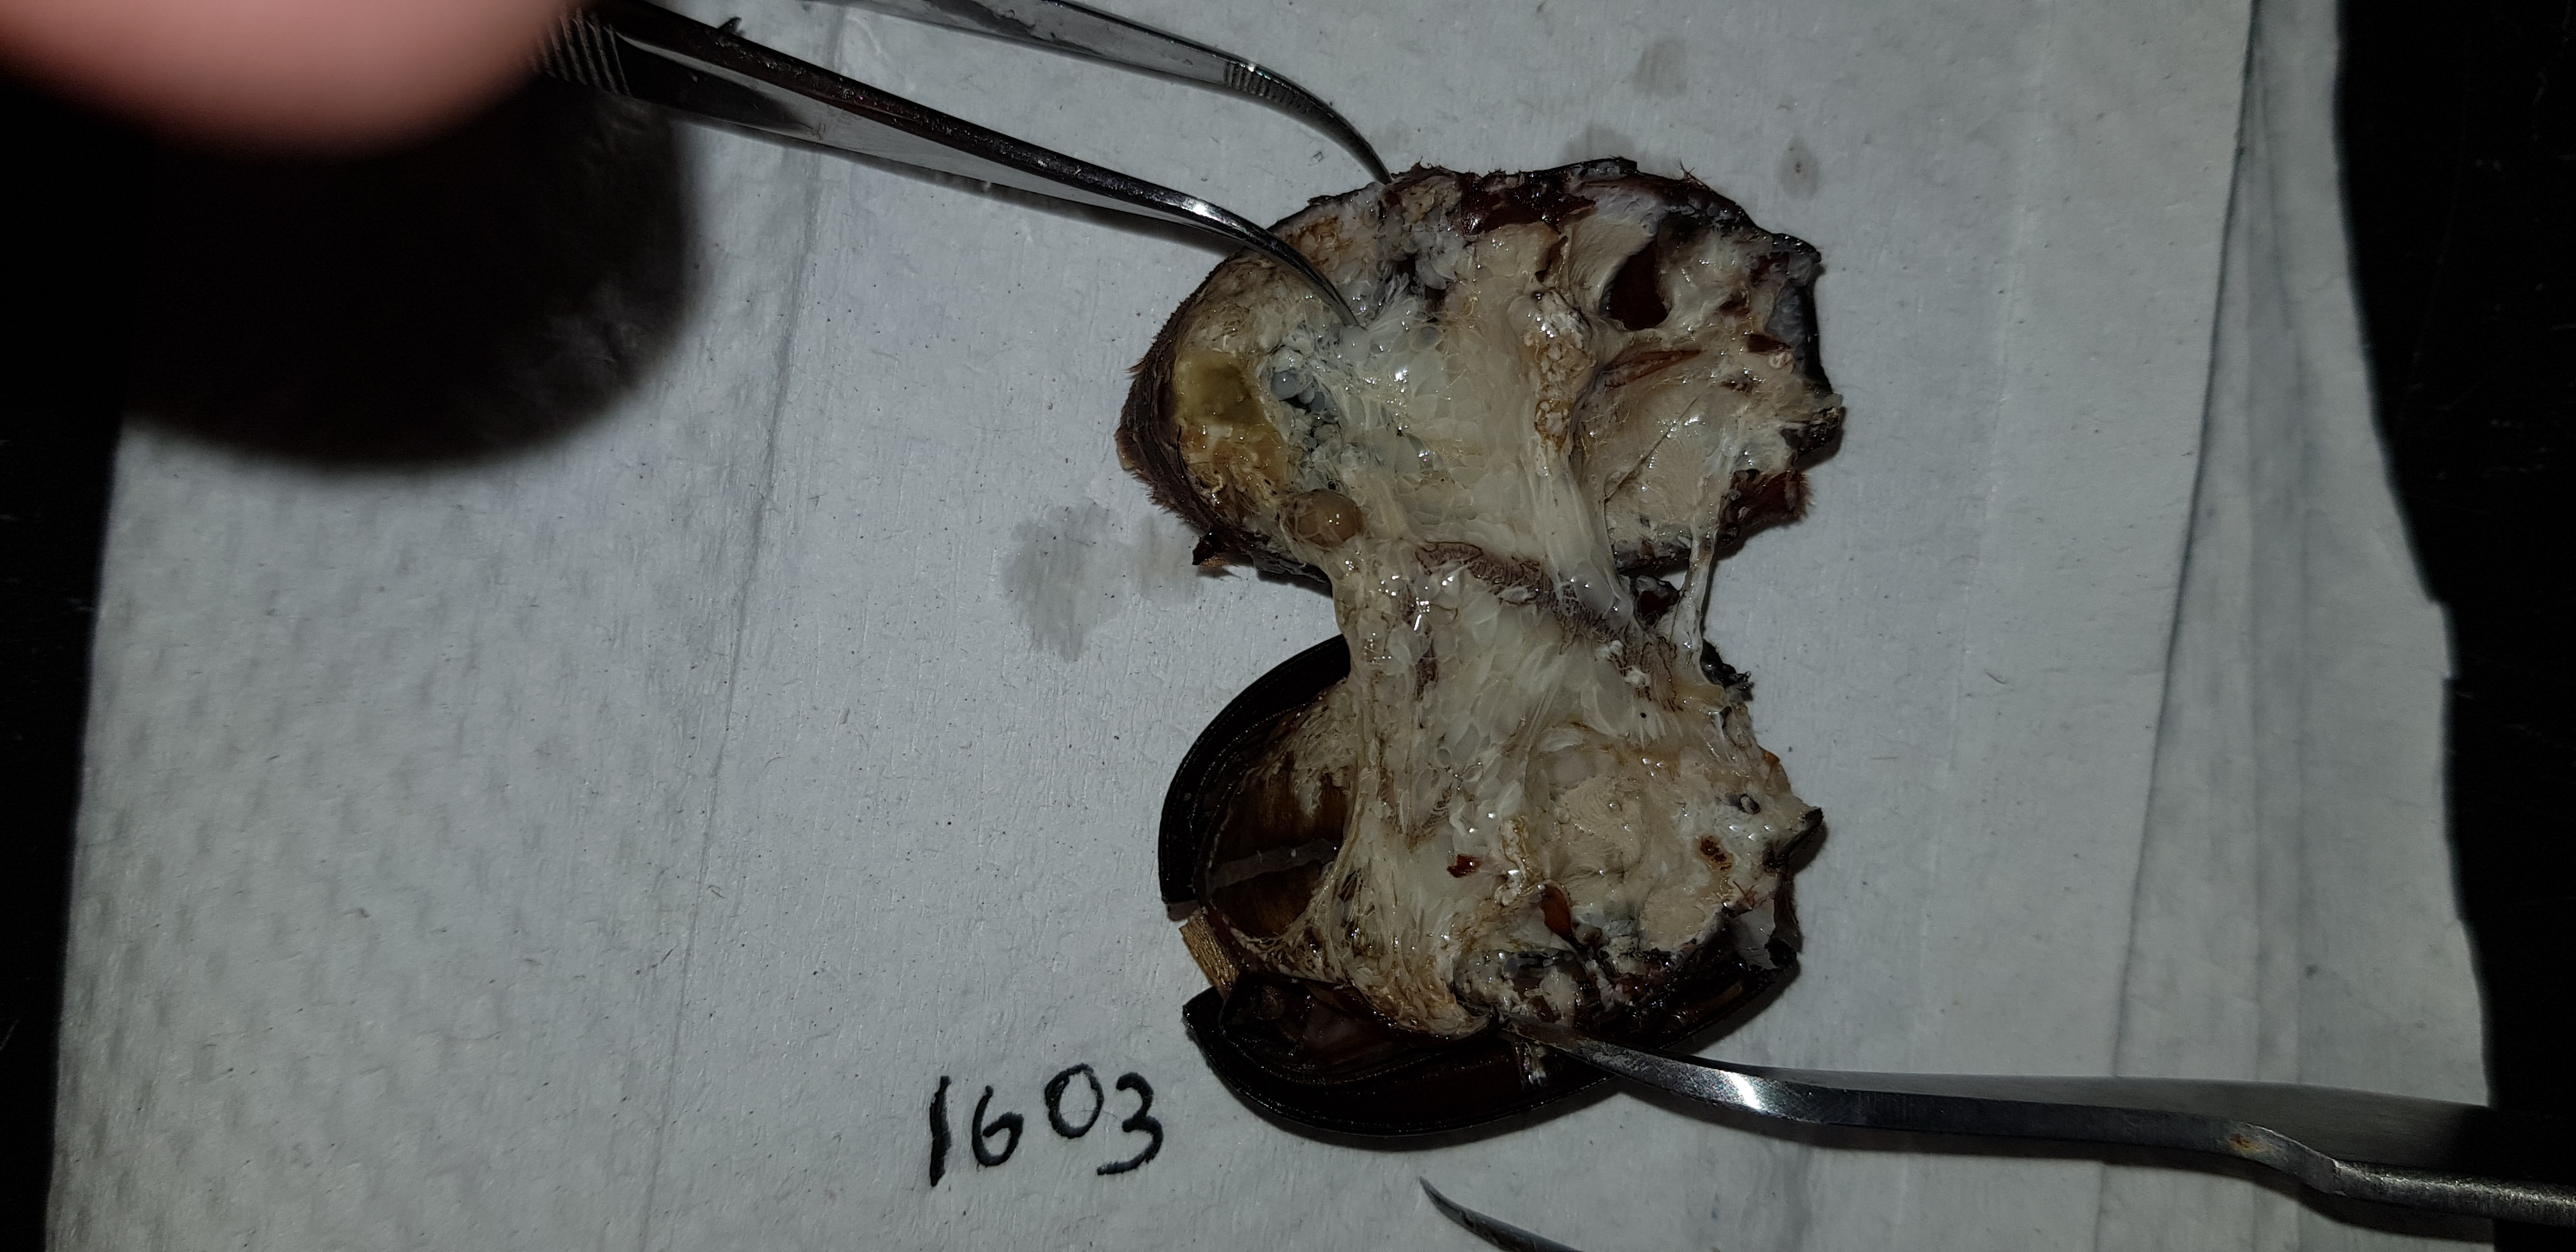
\includegraphics[width=\linewidth, height=\textheight, keepaspectratio]{uploads/btl.pm_image.b9ef3c9106e2af10.447567343220313630335f5265702d3120284849292e6a7067.jpg}
    \caption{Bioassay: DUG42-1; Treatment: heat inactivated; Beetle ID: 52}
\end{figure}
\clearpage

\begin{figure}[h!]
    \centering
    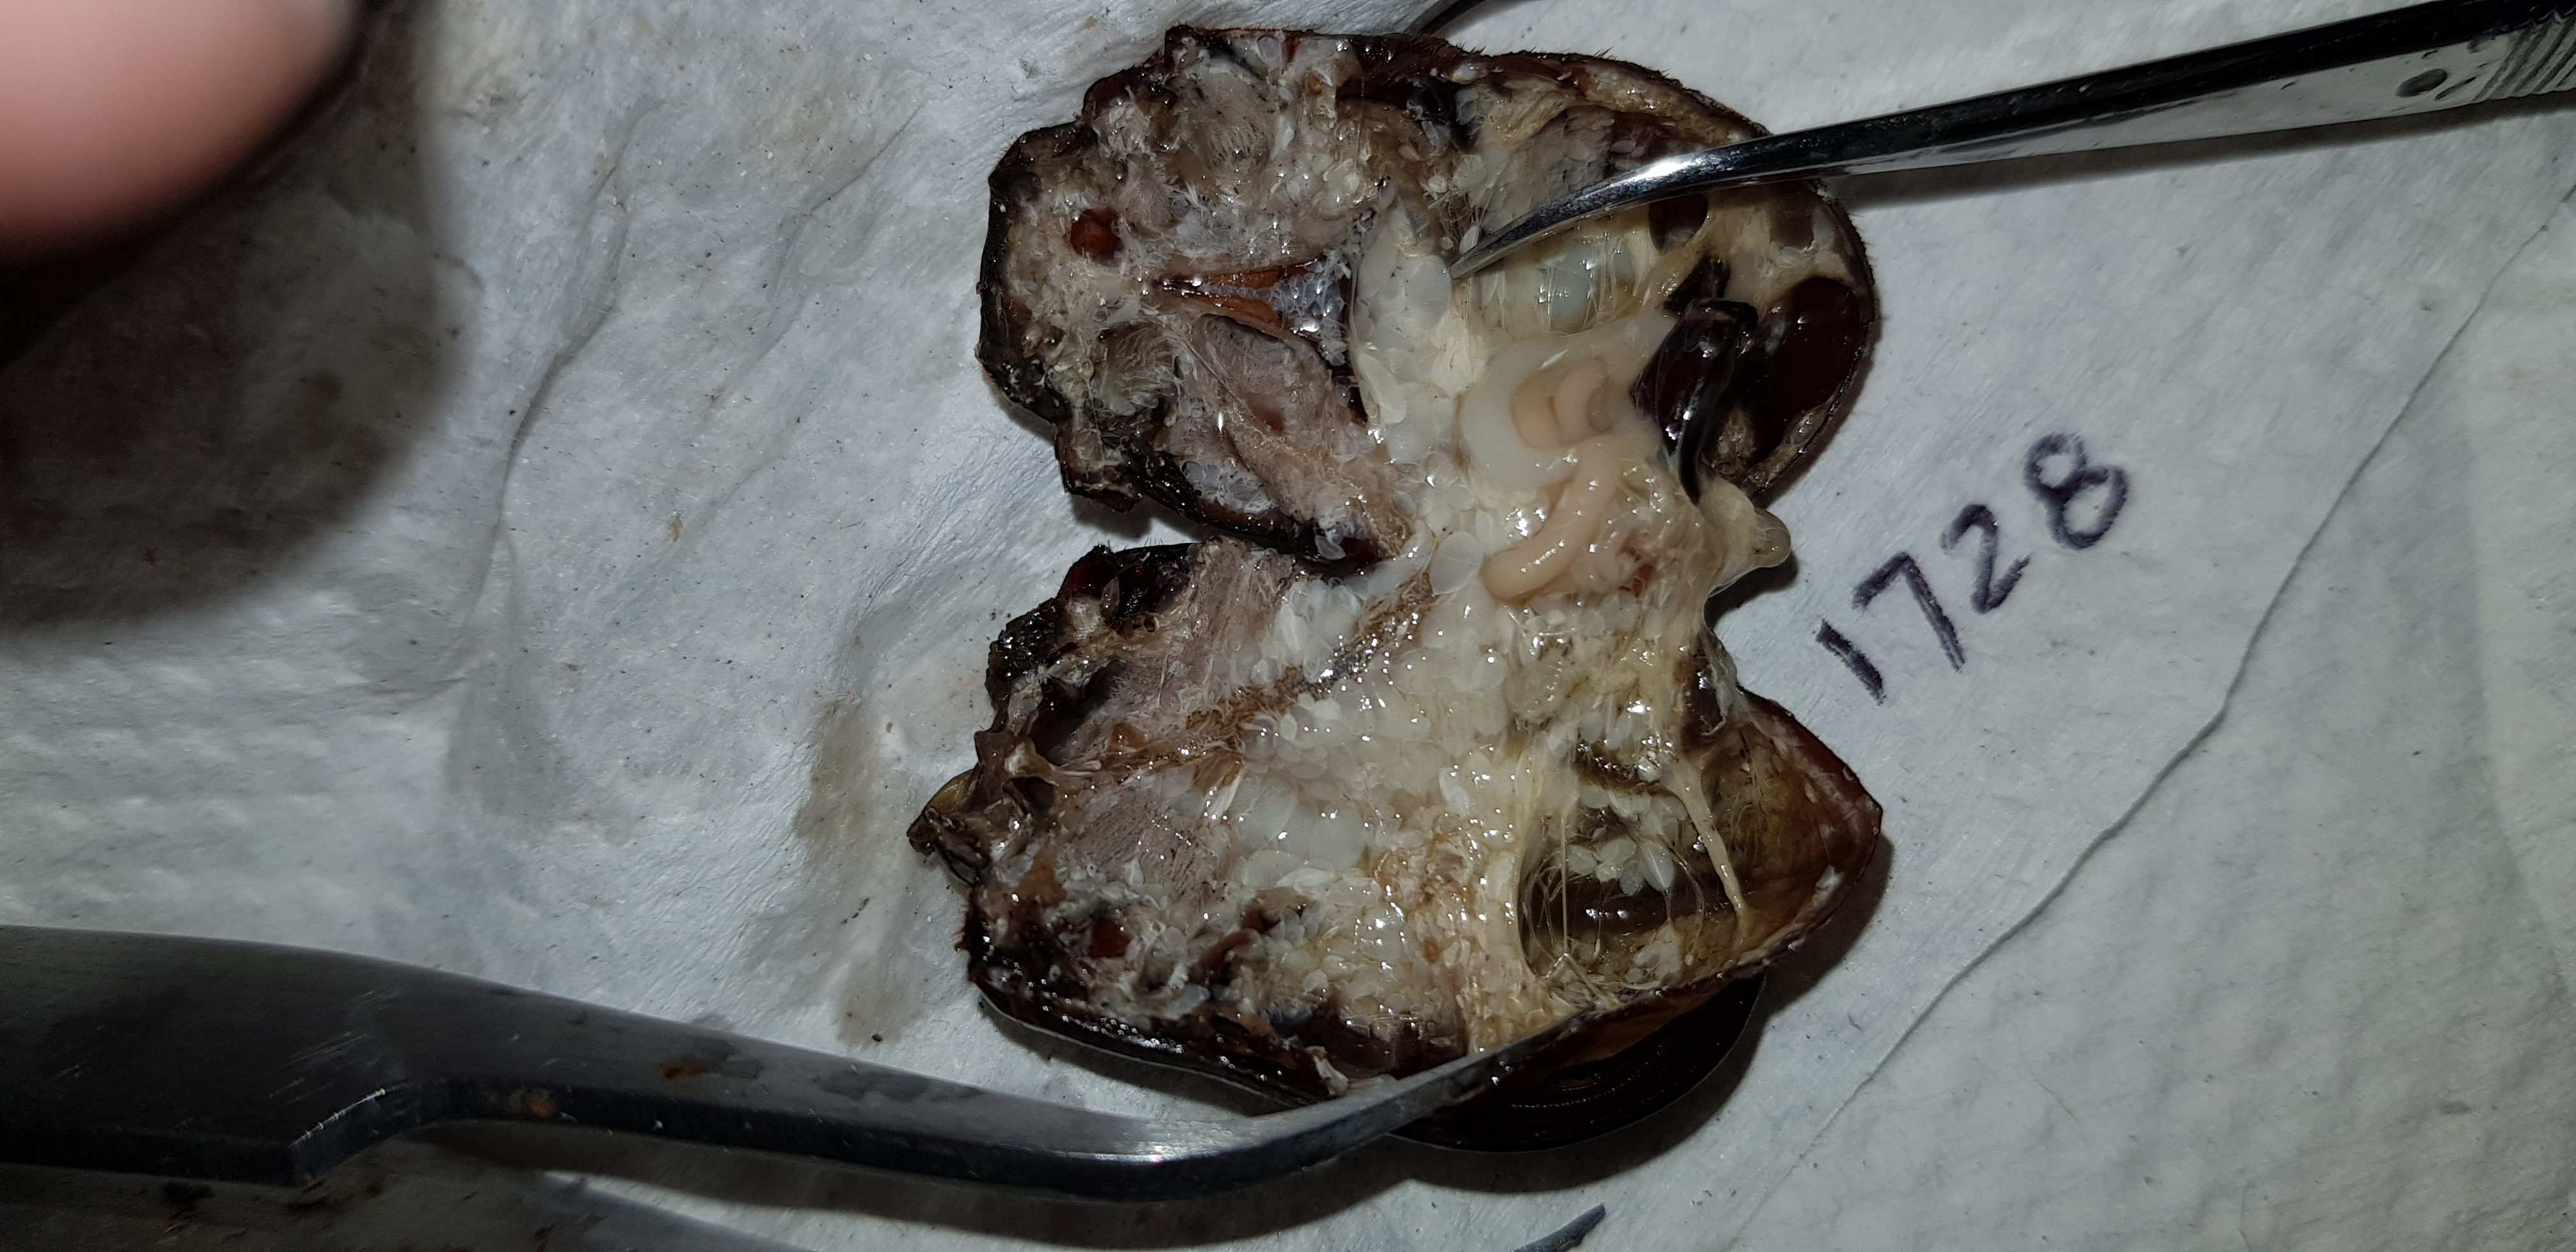
\includegraphics[width=\linewidth, height=\textheight, keepaspectratio]{uploads/btl.pm_image.98f38092242fe55e.447567343220313732385f5265702d3120636f6e74726f6c2e6a7067.jpg}
    \caption{Bioassay: DUG42-1; Treatment: heat inactivated; Beetle ID: 53}
\end{figure}
\clearpage

\begin{figure}[h!]
    \centering
    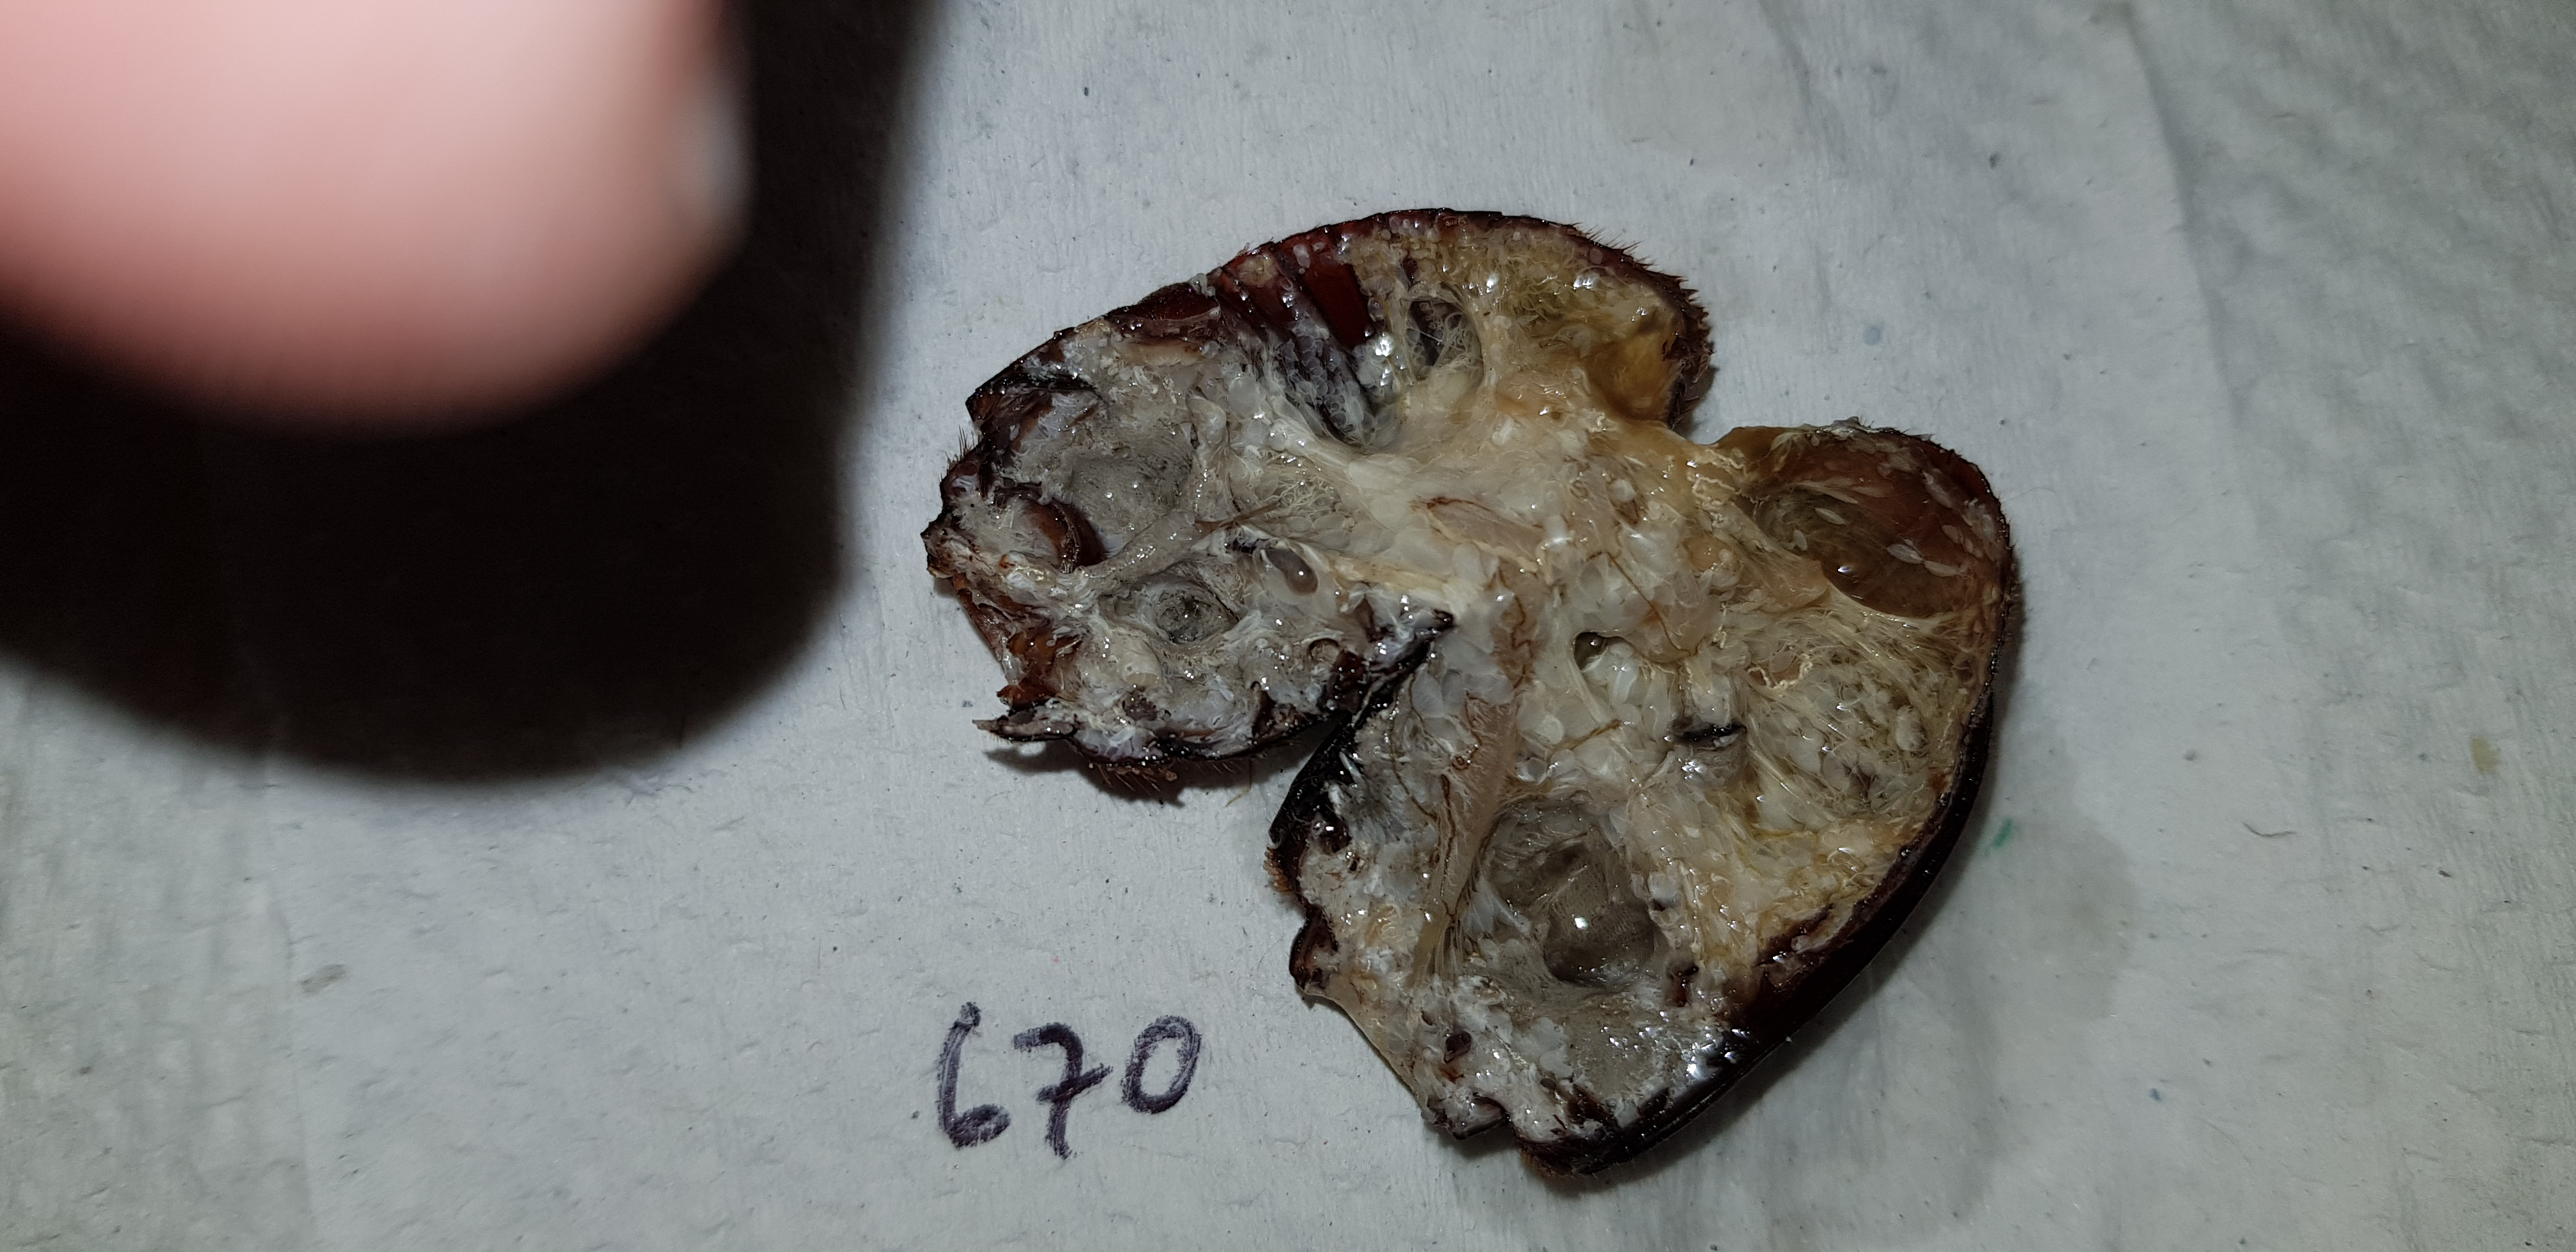
\includegraphics[width=\linewidth, height=\textheight, keepaspectratio]{uploads/btl.pm_image.9ddaa0b244e4bd35.4475673432203637305f5265702d3120636f6e74726f6c2e6a7067.jpg}
    \caption{Bioassay: DUG42-1; Treatment: heat inactivated; Beetle ID: 54}
\end{figure}
\clearpage

\begin{figure}[h!]
    \centering
    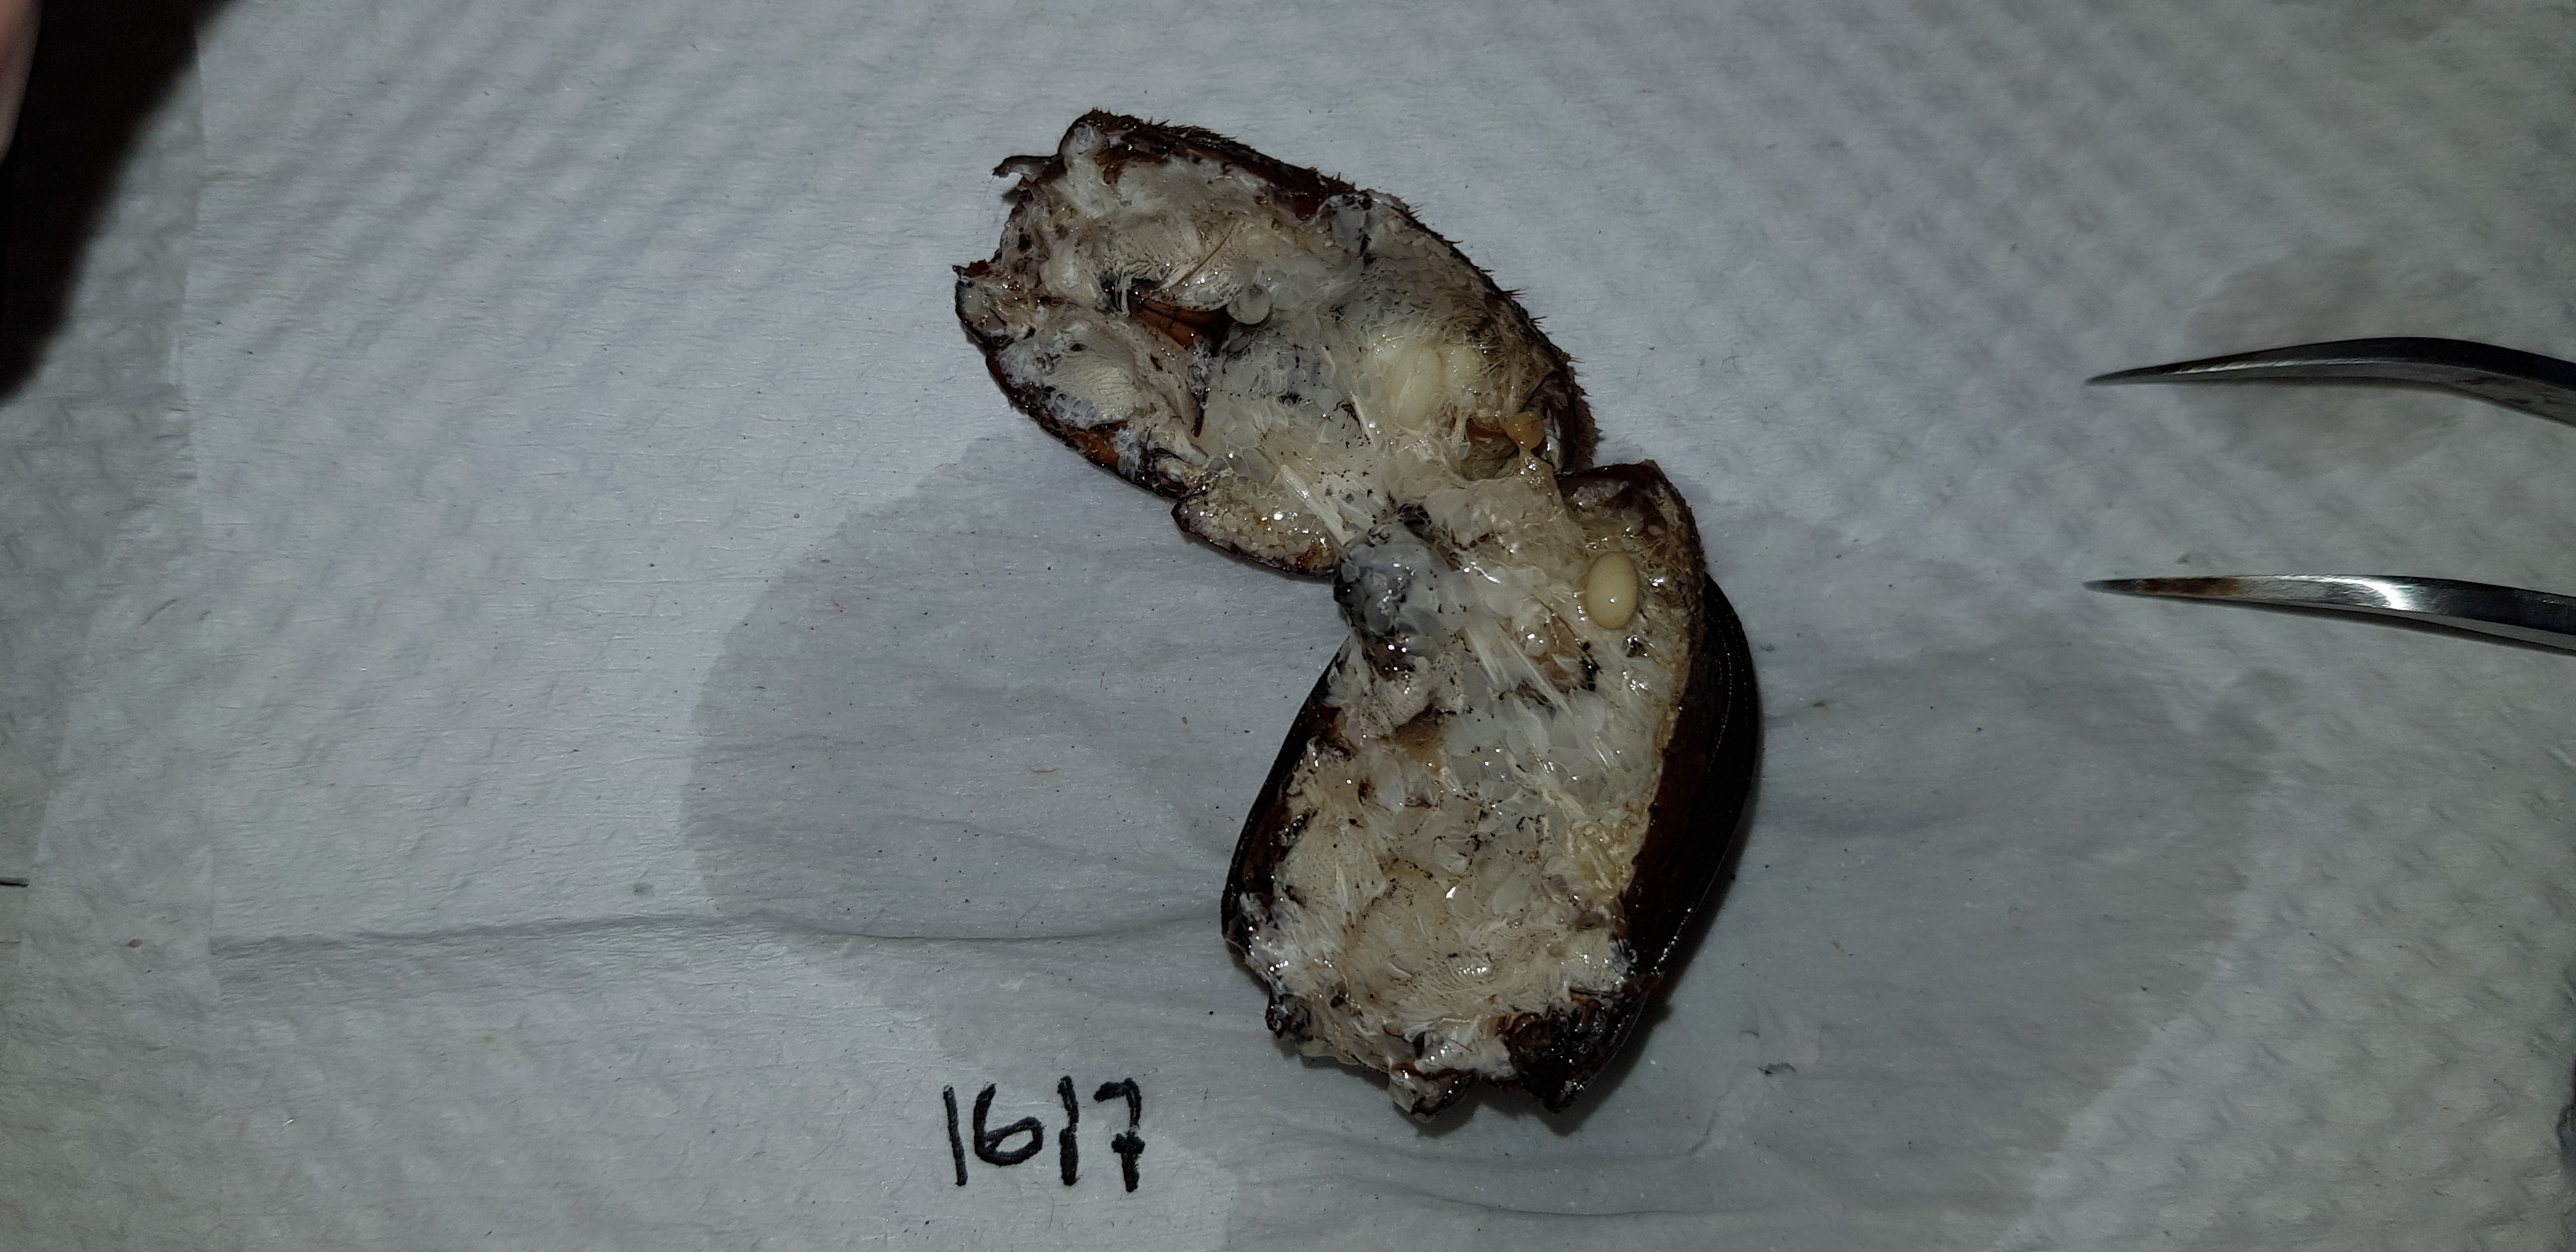
\includegraphics[width=\linewidth, height=\textheight, keepaspectratio]{uploads/btl.pm_image.b43c7102da766f30.447567343220313631375f5265702d3120284849292e6a7067.jpg}
    \caption{Bioassay: DUG42-1; Treatment: heat inactivated; Beetle ID: 55}
\end{figure}
\clearpage

\begin{figure}[h!]
    \centering
    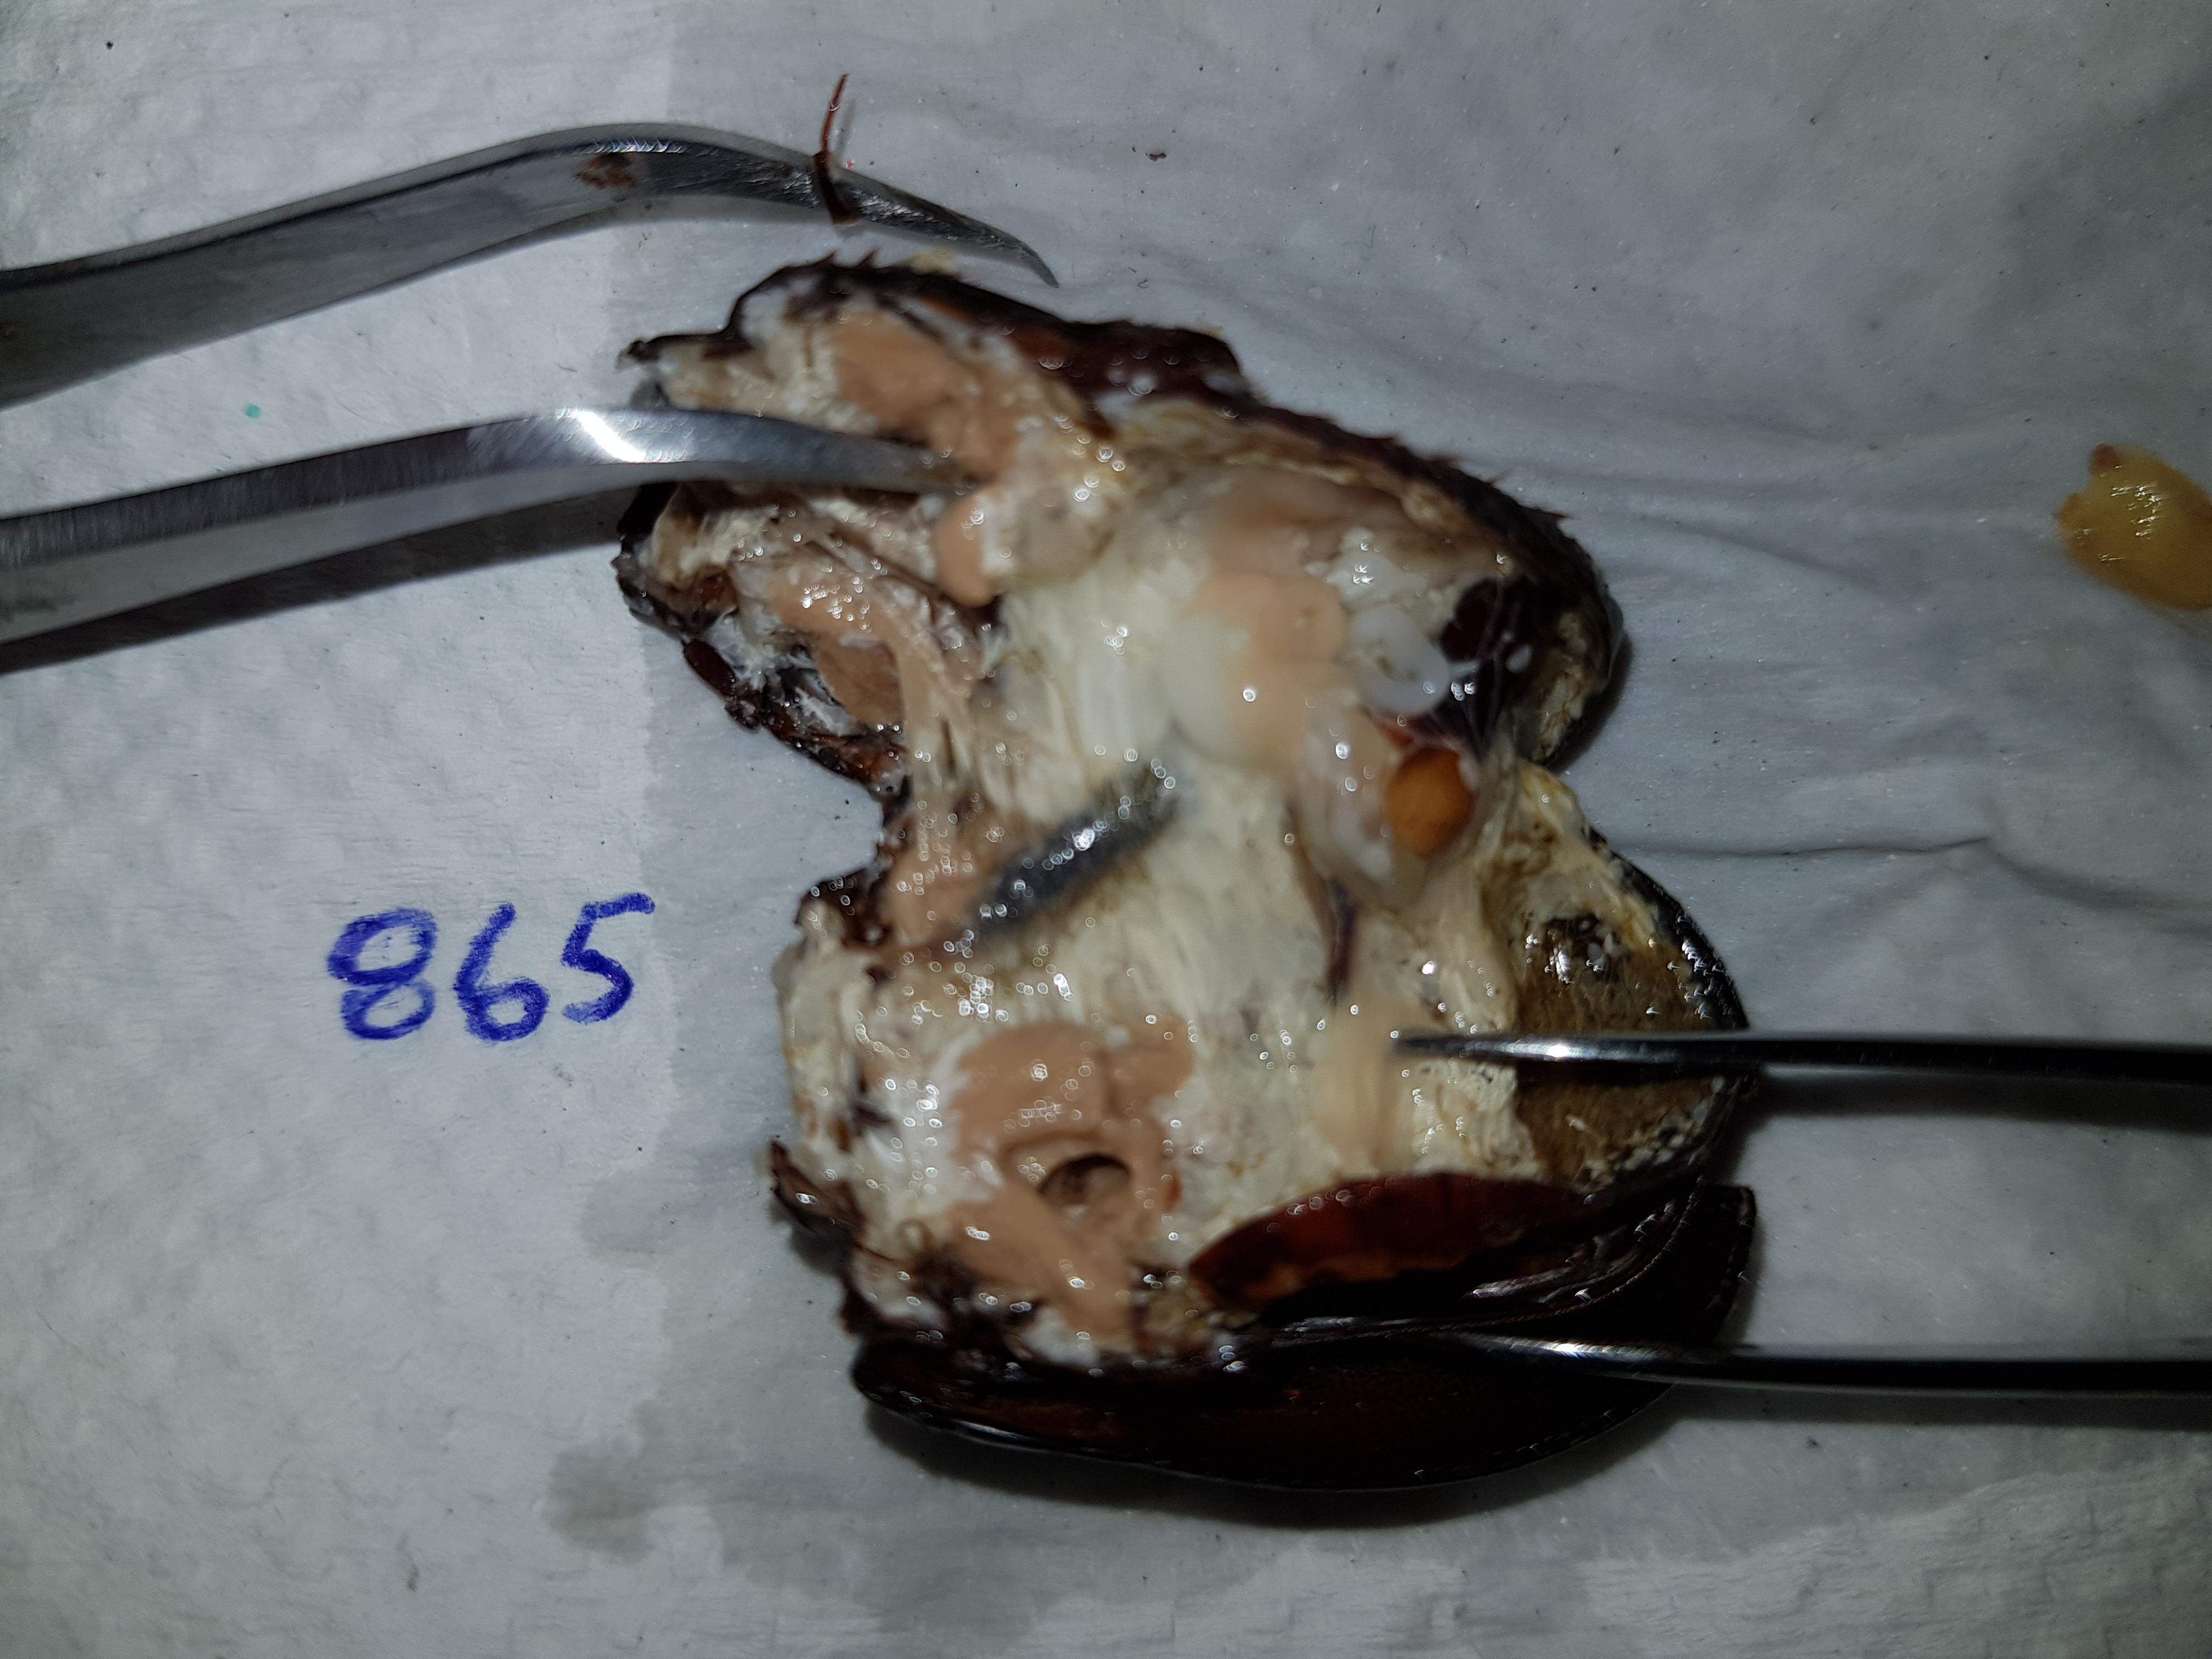
\includegraphics[width=\linewidth, height=\textheight, keepaspectratio]{uploads/btl.pm_image.a8e1877f76b4c77d.4475673432203836355f5265702d3220284849292e6a7067.jpg}
    \caption{Bioassay: DUG42-2; Treatment: heat inactivated; Beetle ID: 66}
\end{figure}
\clearpage

\begin{figure}[h!]
    \centering
    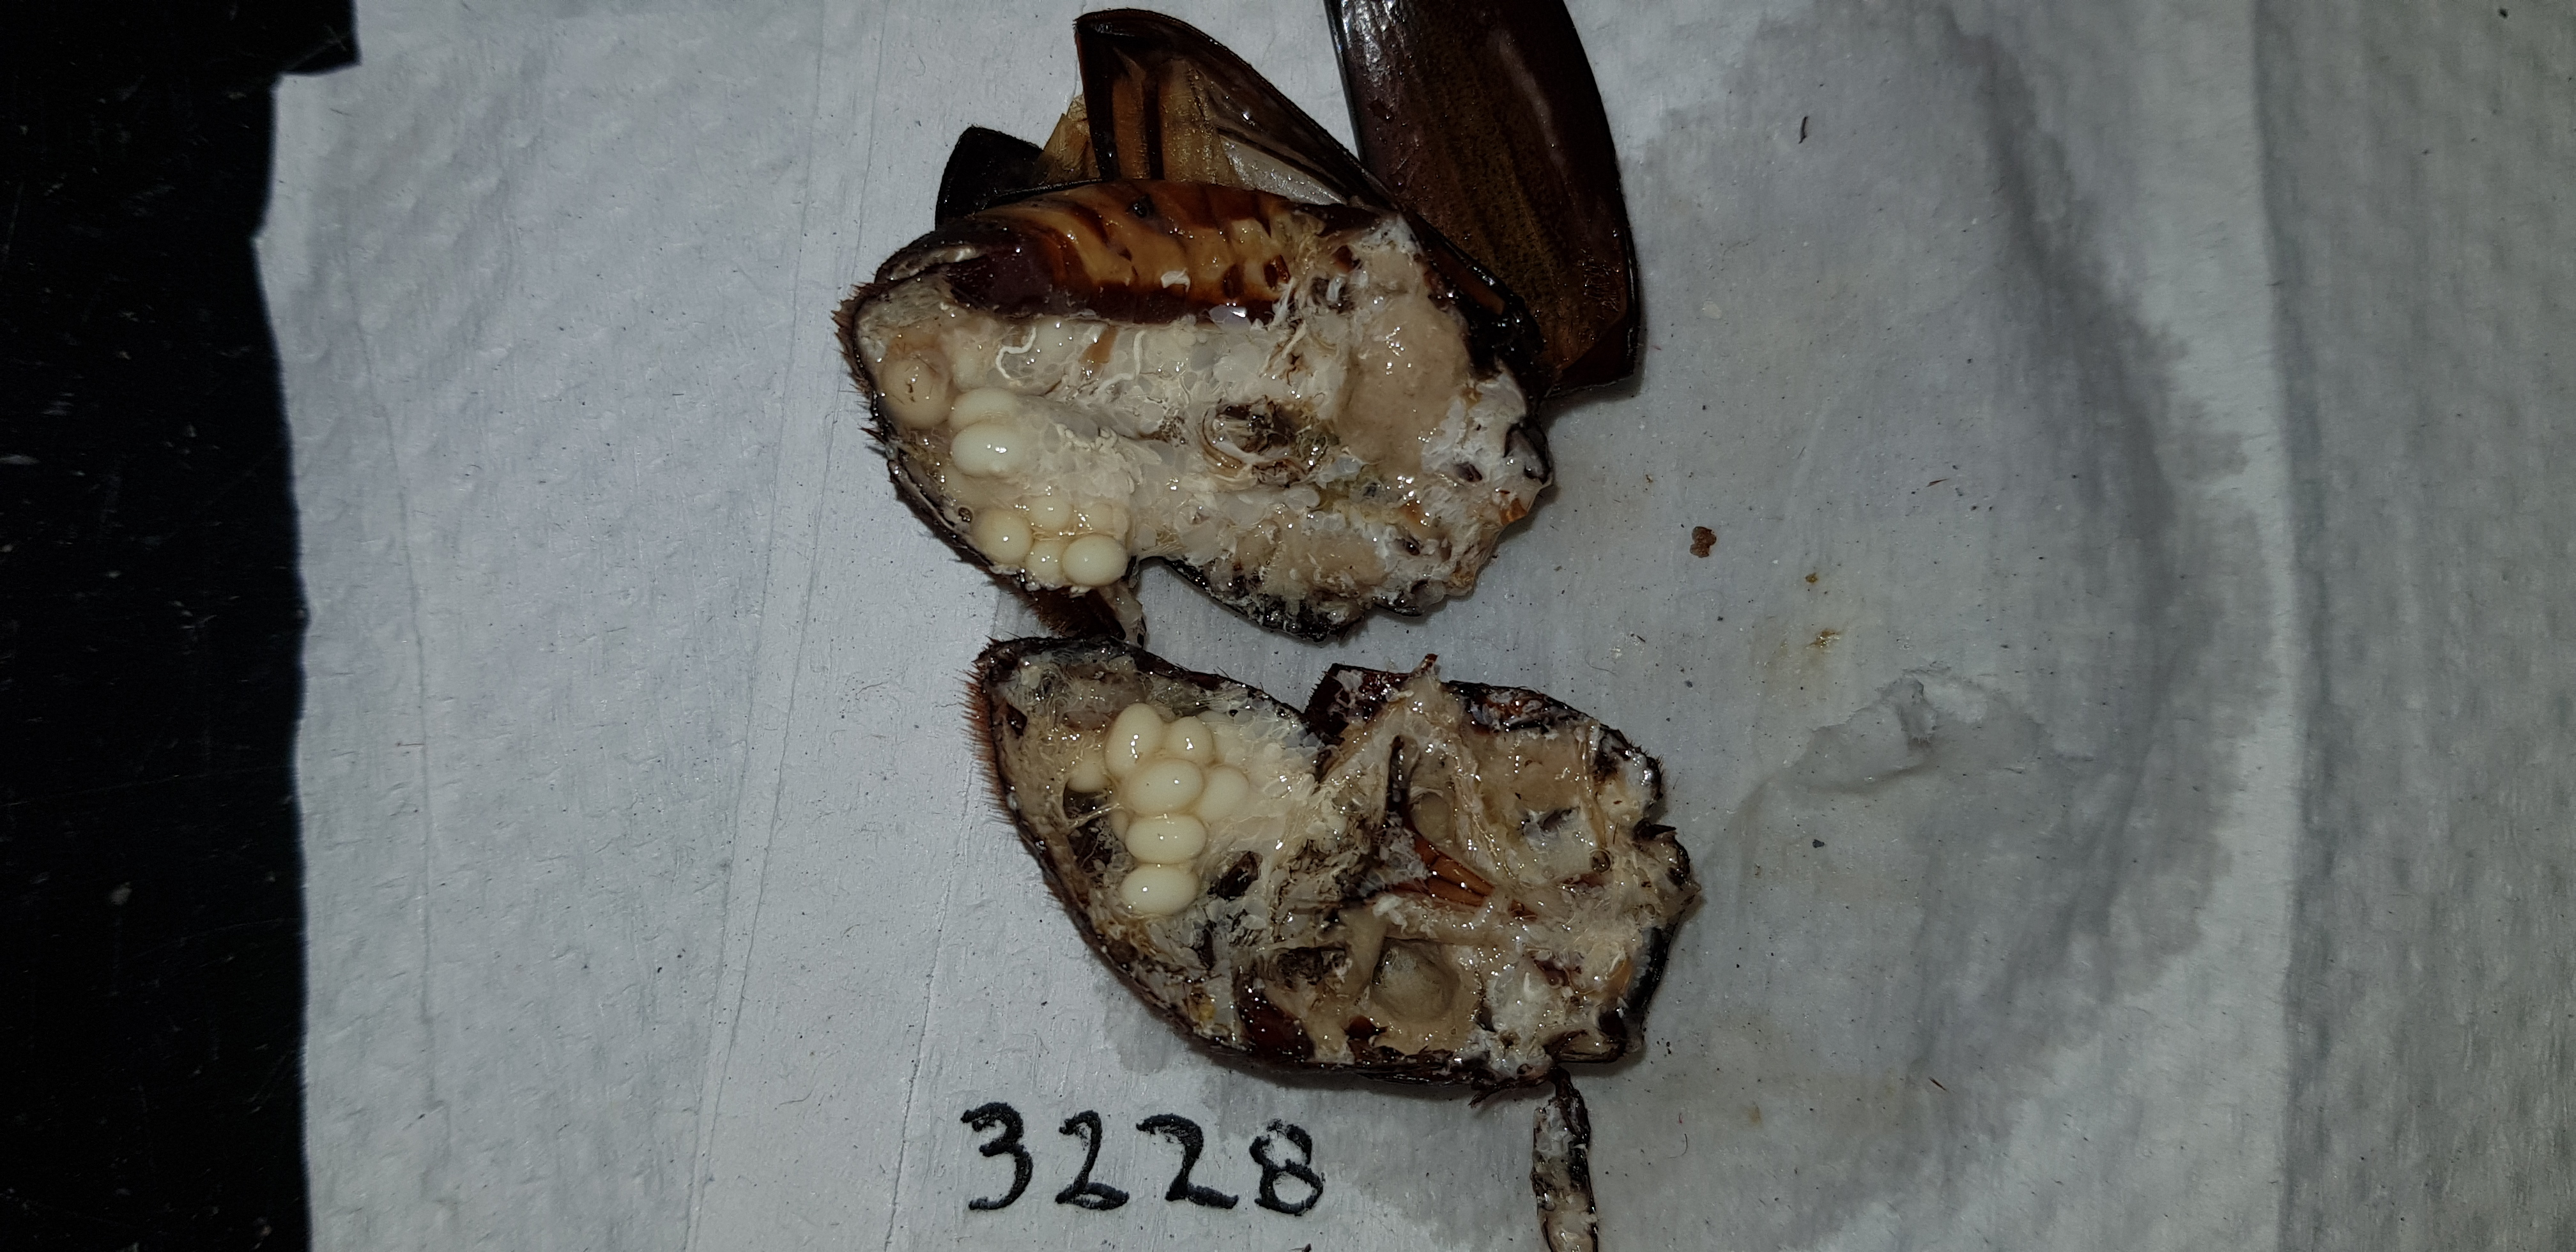
\includegraphics[width=\linewidth, height=\textheight, keepaspectratio]{uploads/btl.pm_image.a74f3b6001fab6de.447567343220333232385f5265702d3220284849292e6a7067.jpg}
    \caption{Bioassay: DUG42-2; Treatment: heat inactivated; Beetle ID: 67}
\end{figure}
\clearpage

\begin{figure}[h!]
    \centering
    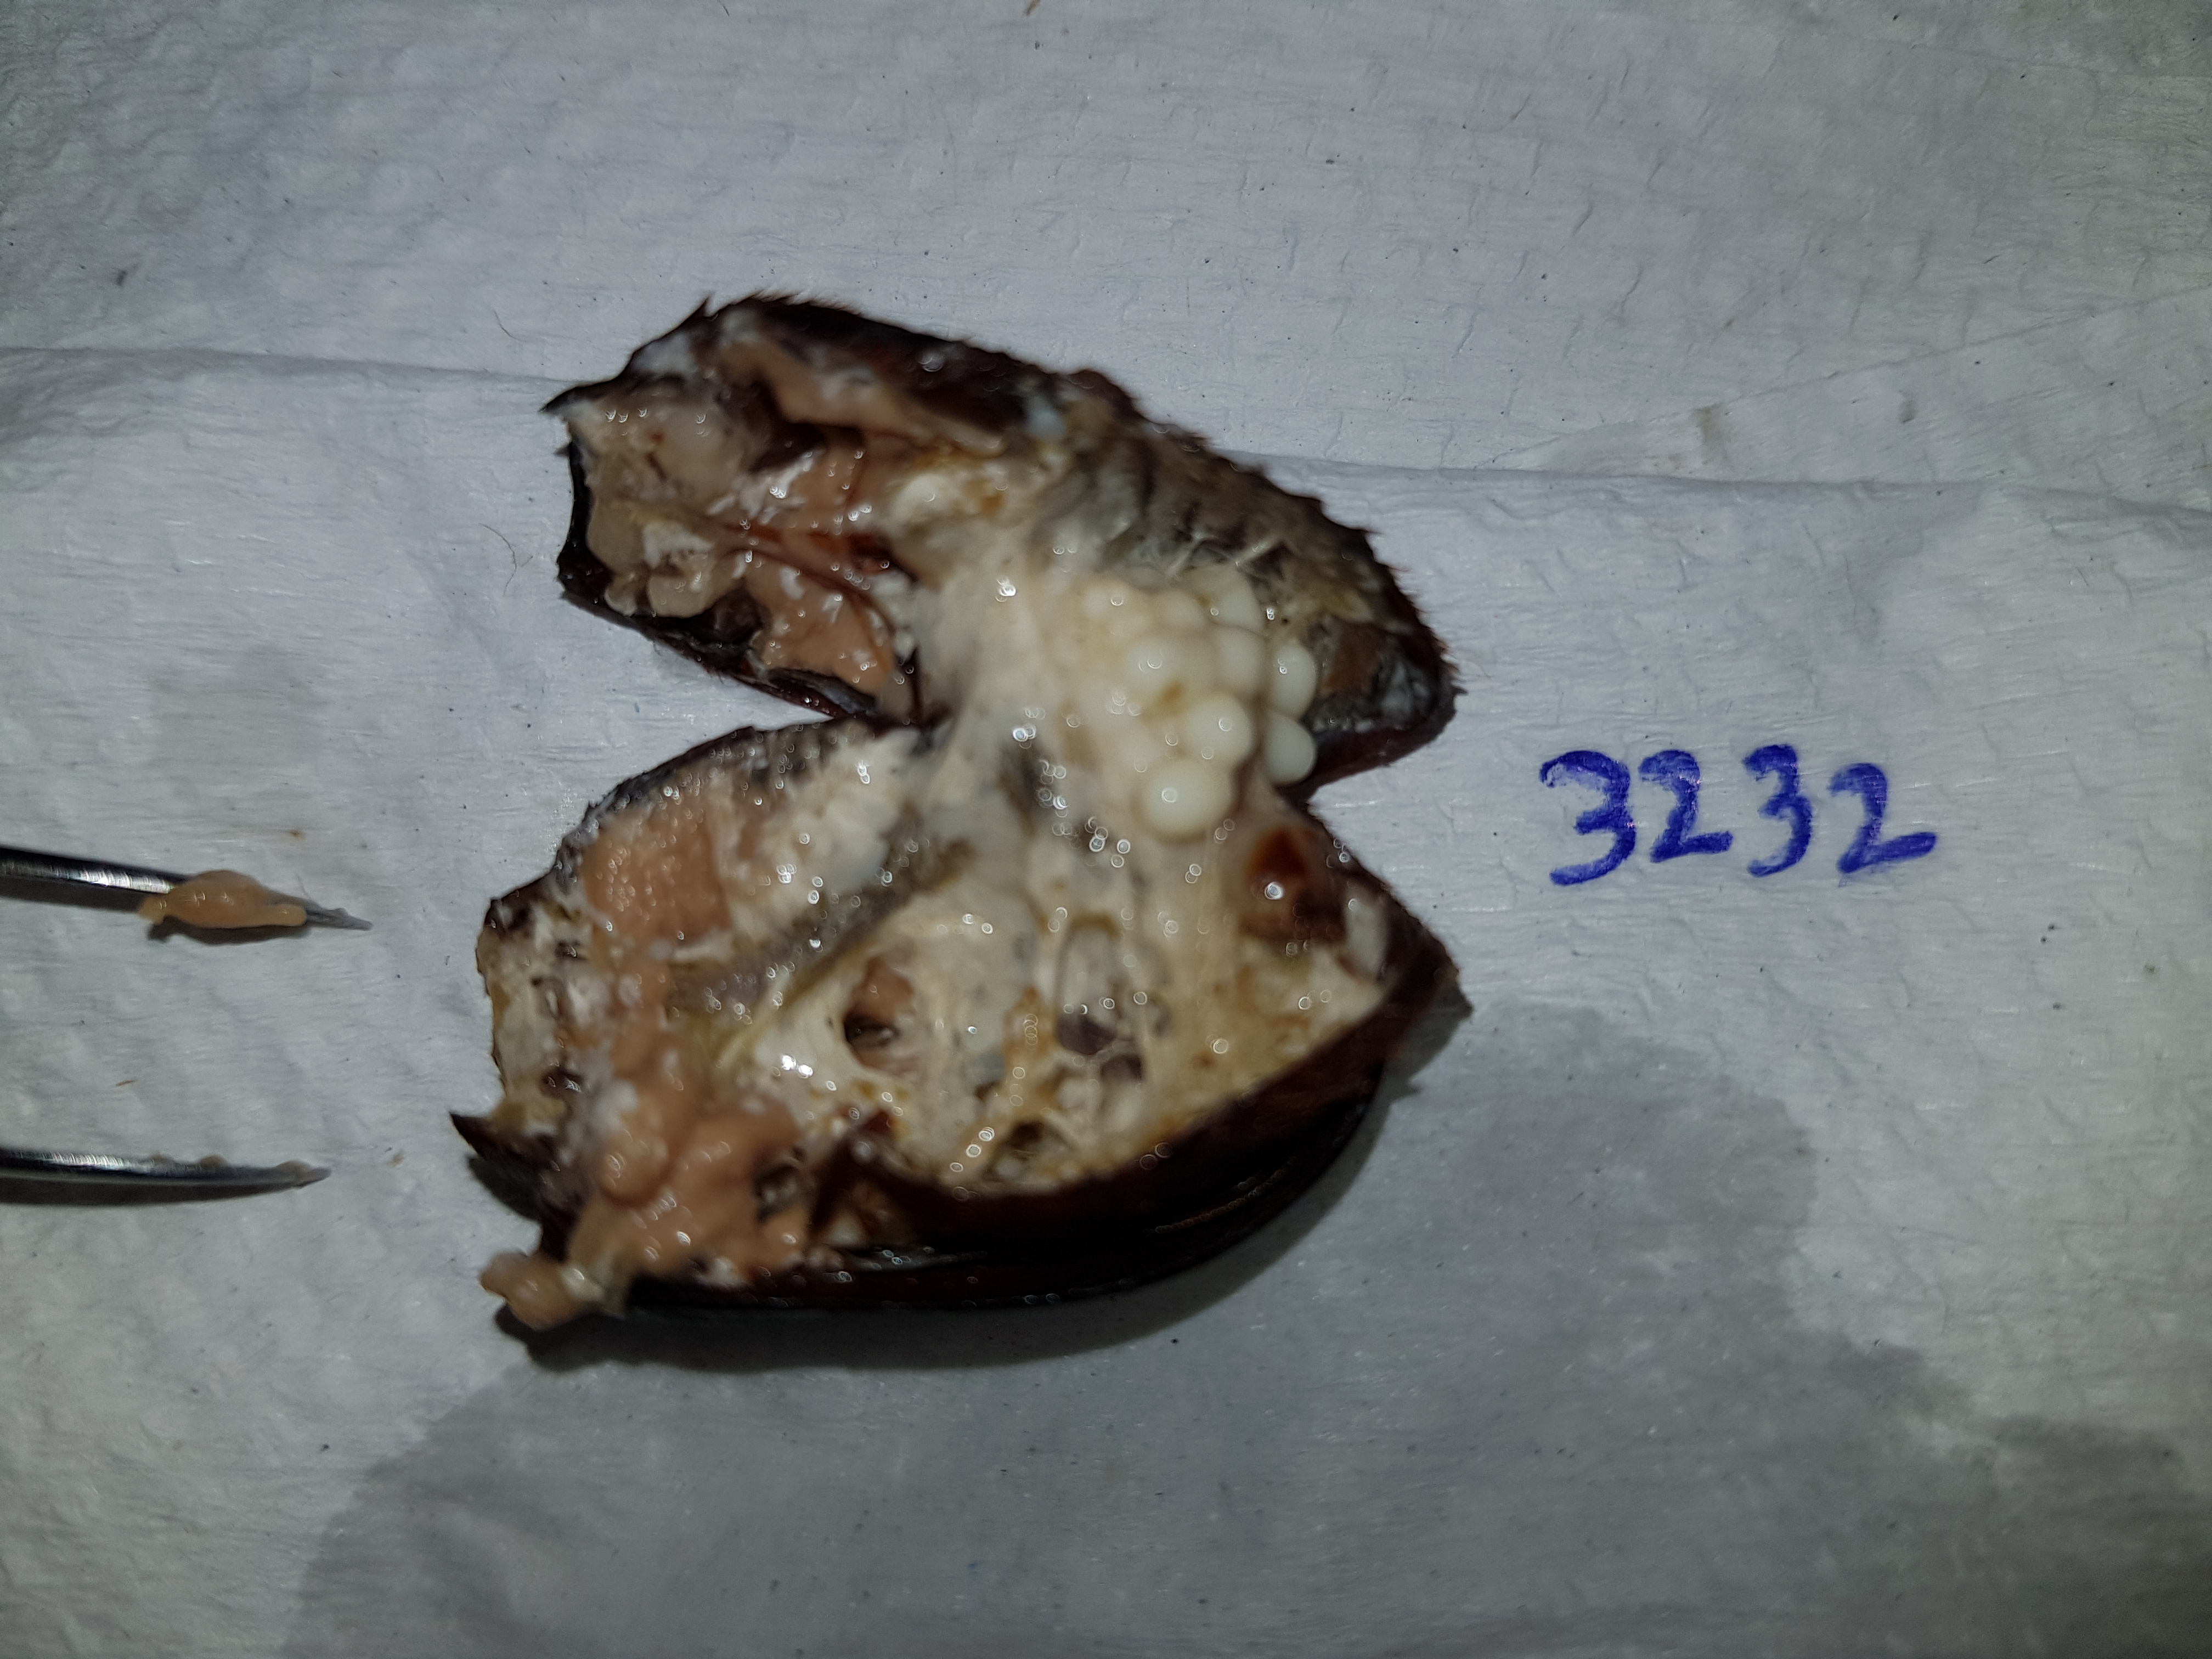
\includegraphics[width=\linewidth, height=\textheight, keepaspectratio]{uploads/btl.pm_image.bd48eeaa05f7b7b1.447567343220333233325f5265702d3220284849292e6a7067.jpg}
    \caption{Bioassay: DUG42-2; Treatment: heat inactivated; Beetle ID: 68}
\end{figure}
\clearpage

\begin{figure}[h!]
    \centering
    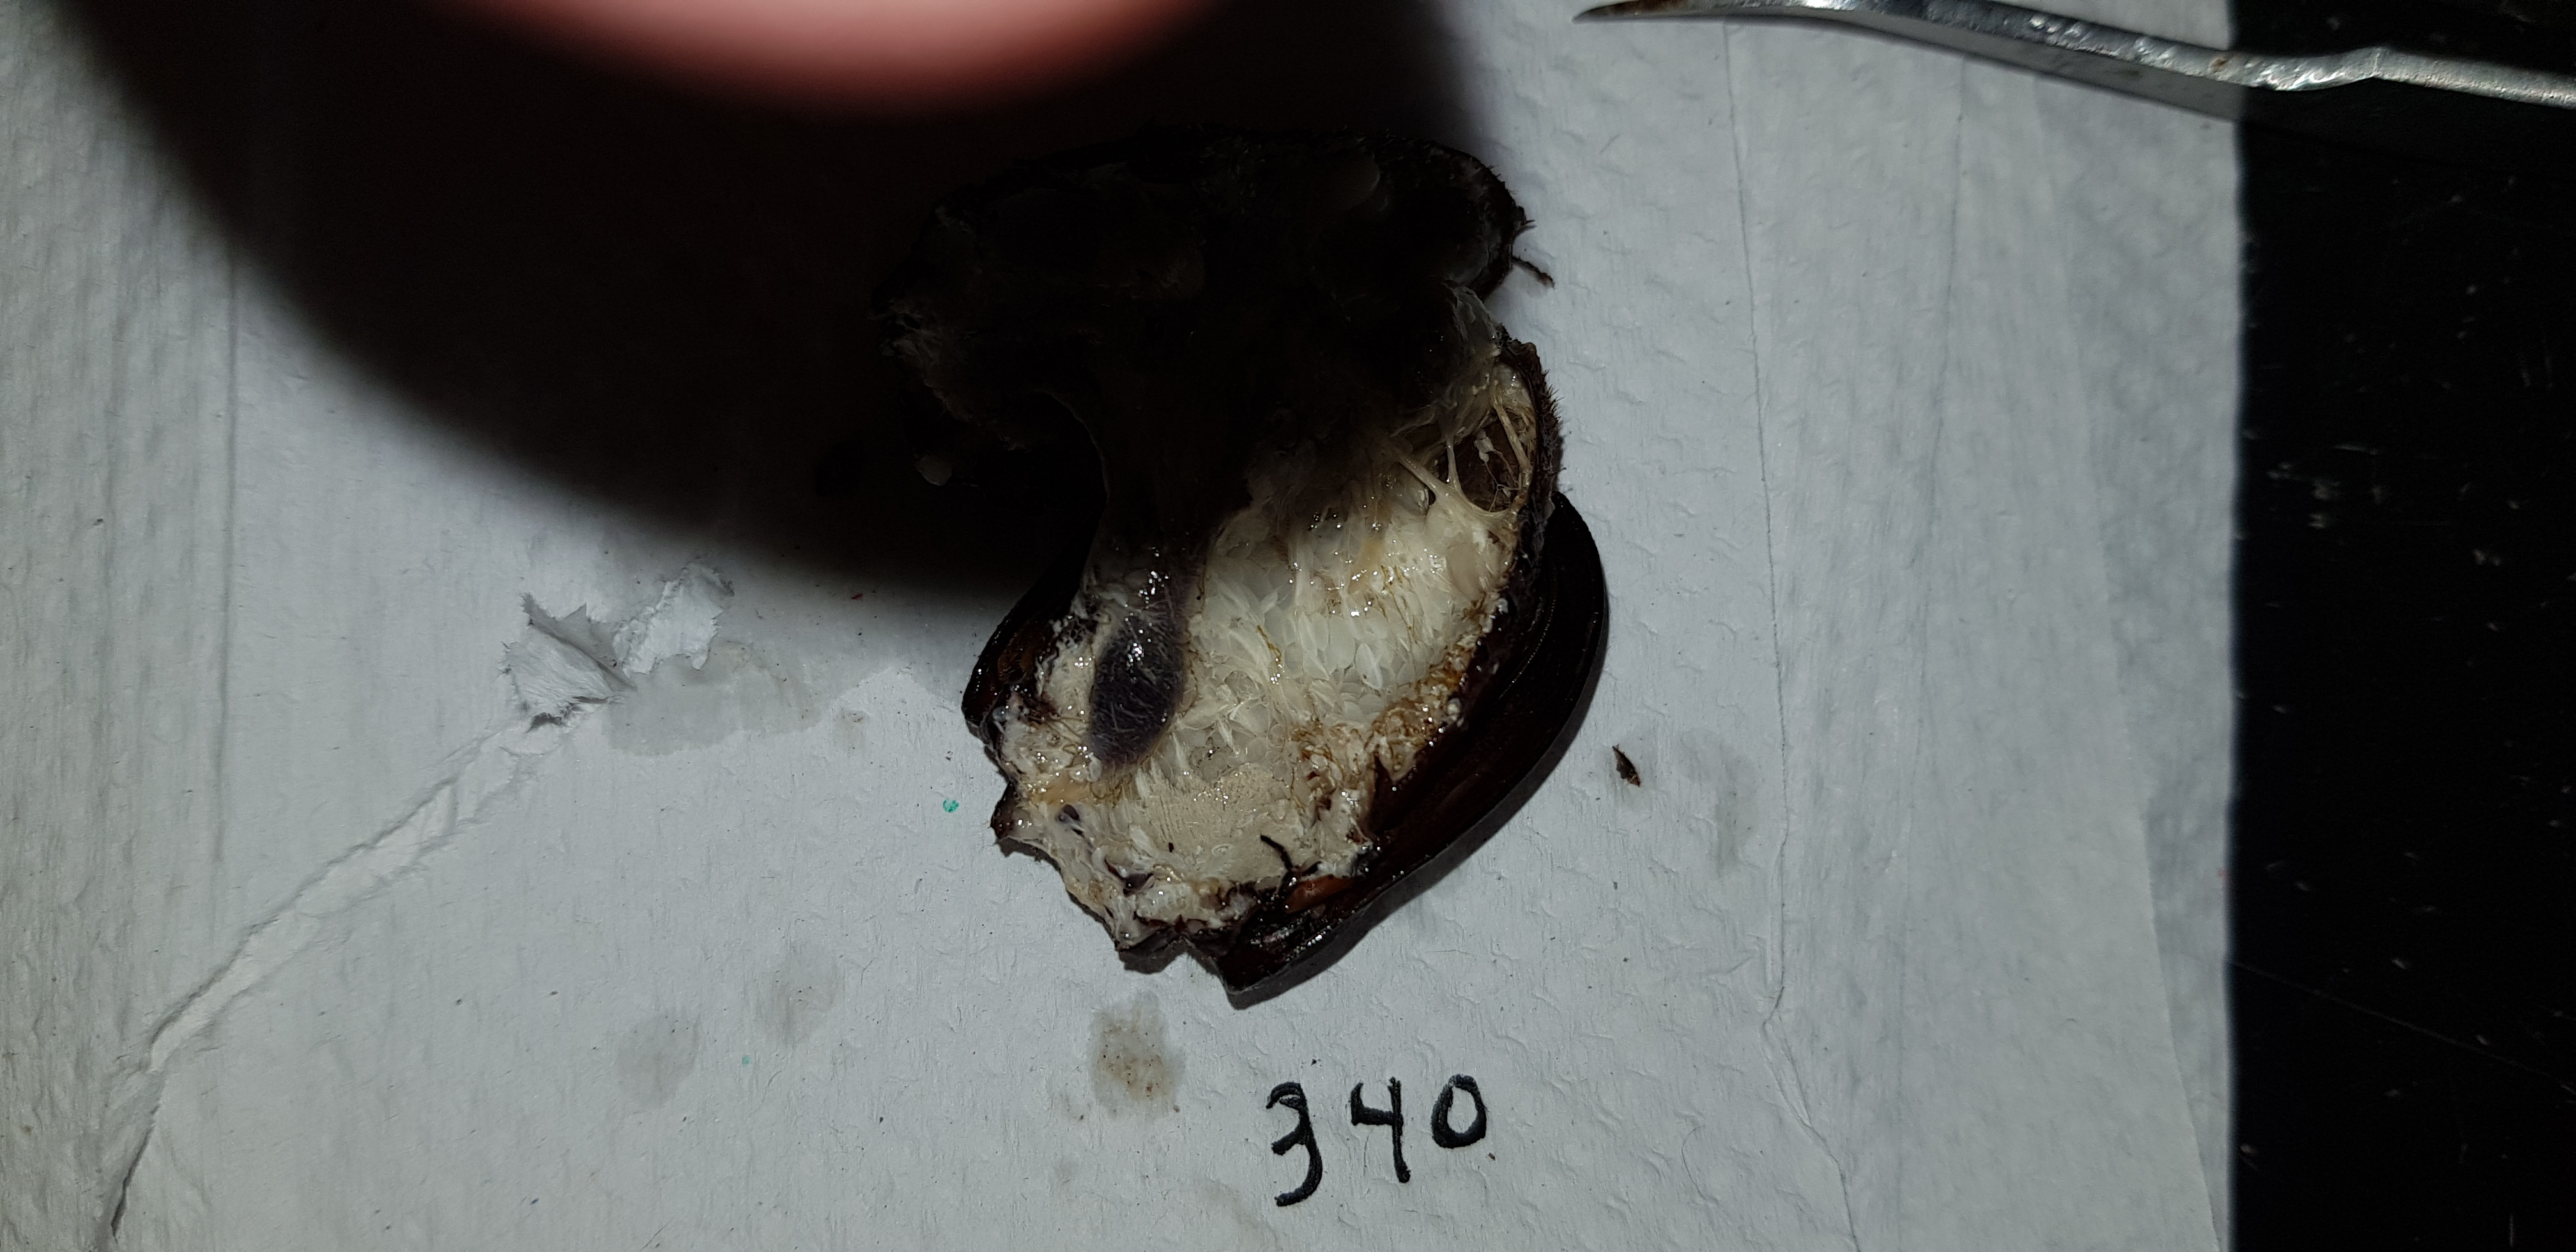
\includegraphics[width=\linewidth, height=\textheight, keepaspectratio]{uploads/btl.pm_image.b9ceff1fc826f7c3.4475673432203334305f5265702d3220284849292e6a7067.jpg}
    \caption{Bioassay: DUG42-2; Treatment: heat inactivated; Beetle ID: 69}
\end{figure}
\clearpage

\begin{figure}[h!]
    \centering
    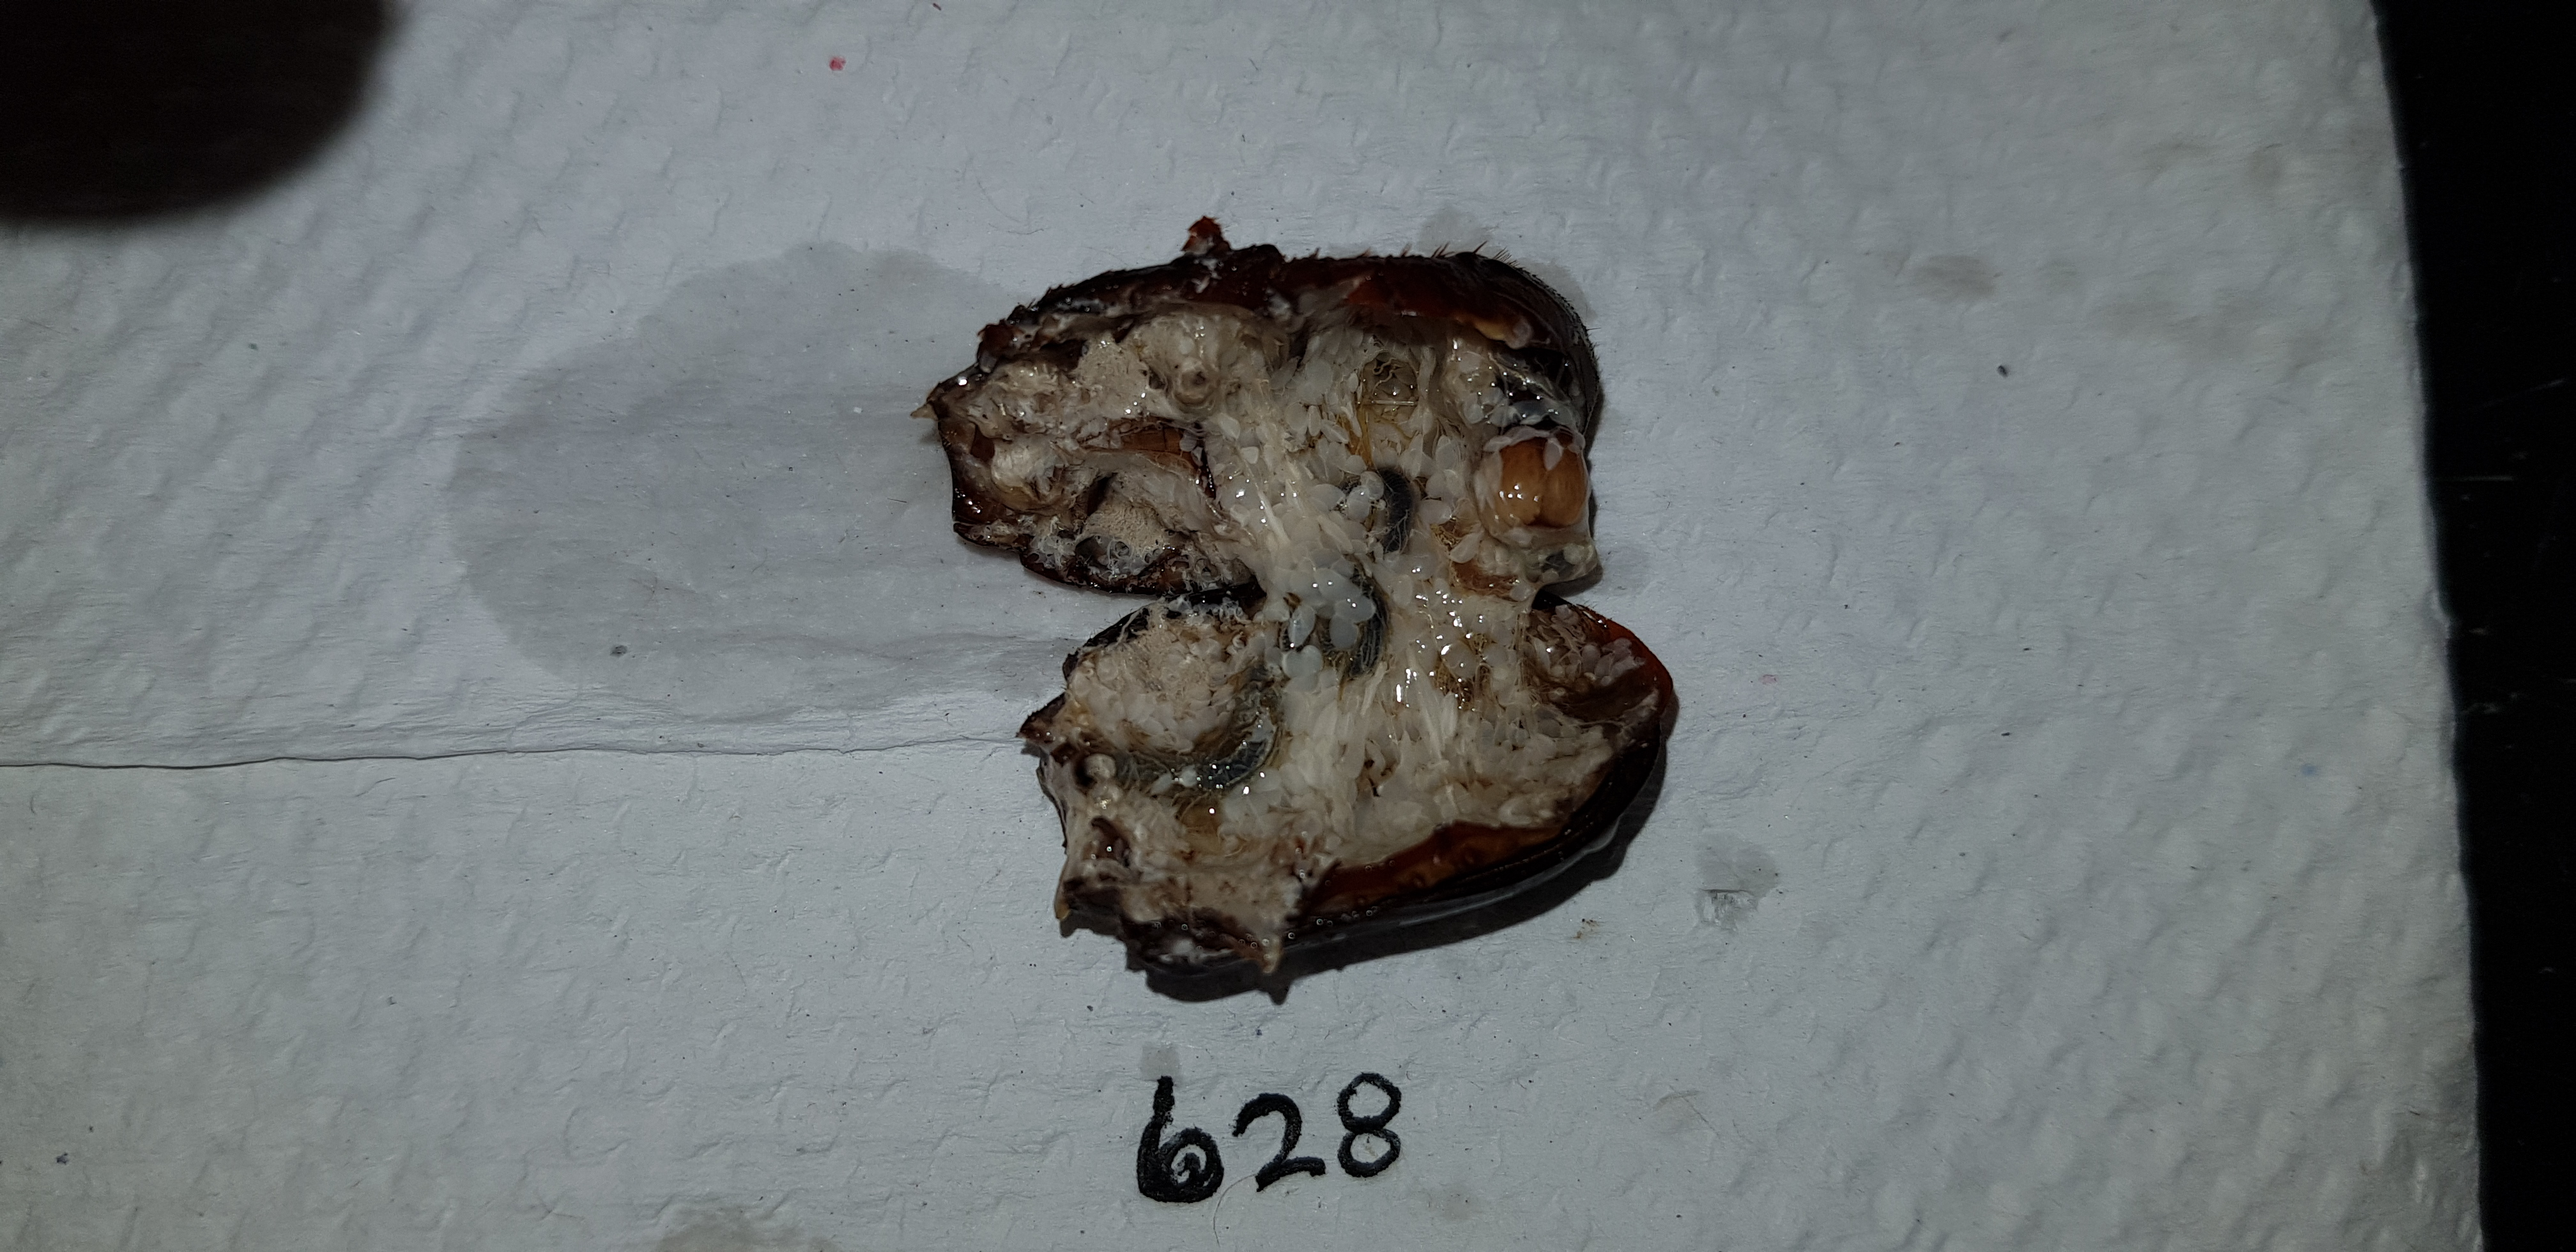
\includegraphics[width=\linewidth, height=\textheight, keepaspectratio]{uploads/btl.pm_image.804a1fbe4c486a85.4475673432203632385f5265702d3220284849292e6a7067.jpg}
    \caption{Bioassay: DUG42-2; Treatment: heat inactivated; Beetle ID: 70}
\end{figure}
\clearpage

\subsection{virus}

\begin{figure}[h!]
    \centering
    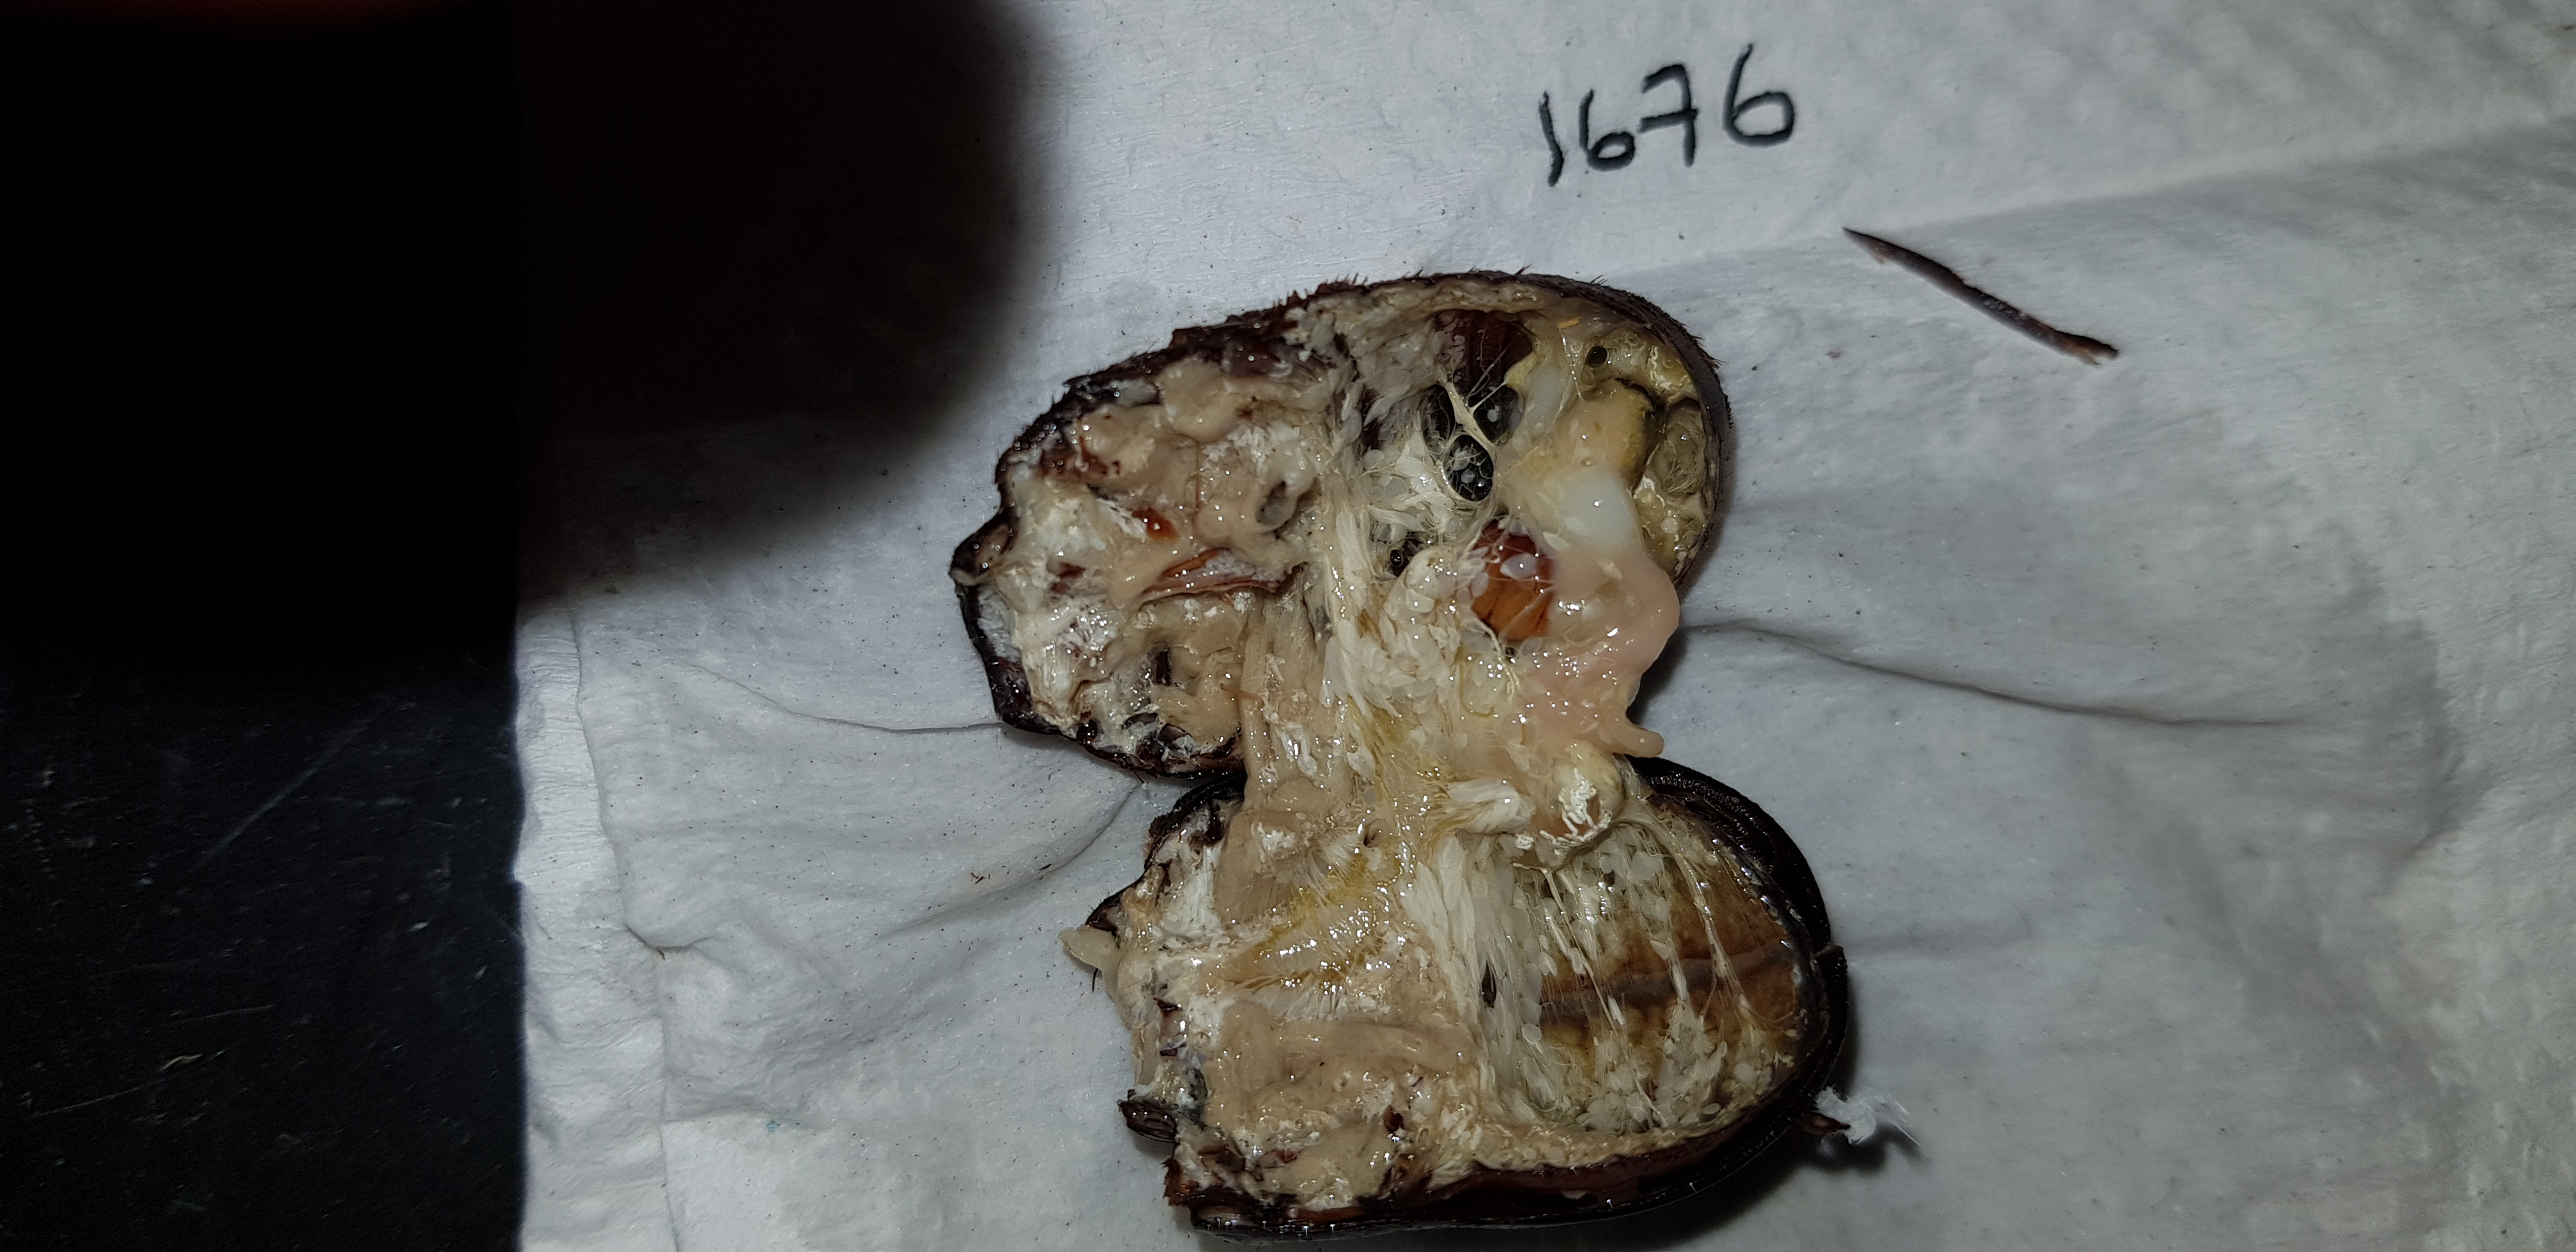
\includegraphics[width=\linewidth, height=\textheight, keepaspectratio]{uploads/btl.pm_image.b3bd14df70606ca8.447567343220313637365f5265702d312076697275732e6a7067.jpg}
    \caption{Bioassay: DUG42-1; Treatment: virus; Beetle ID: 56}
\end{figure}
\clearpage

\begin{figure}[h!]
    \centering
    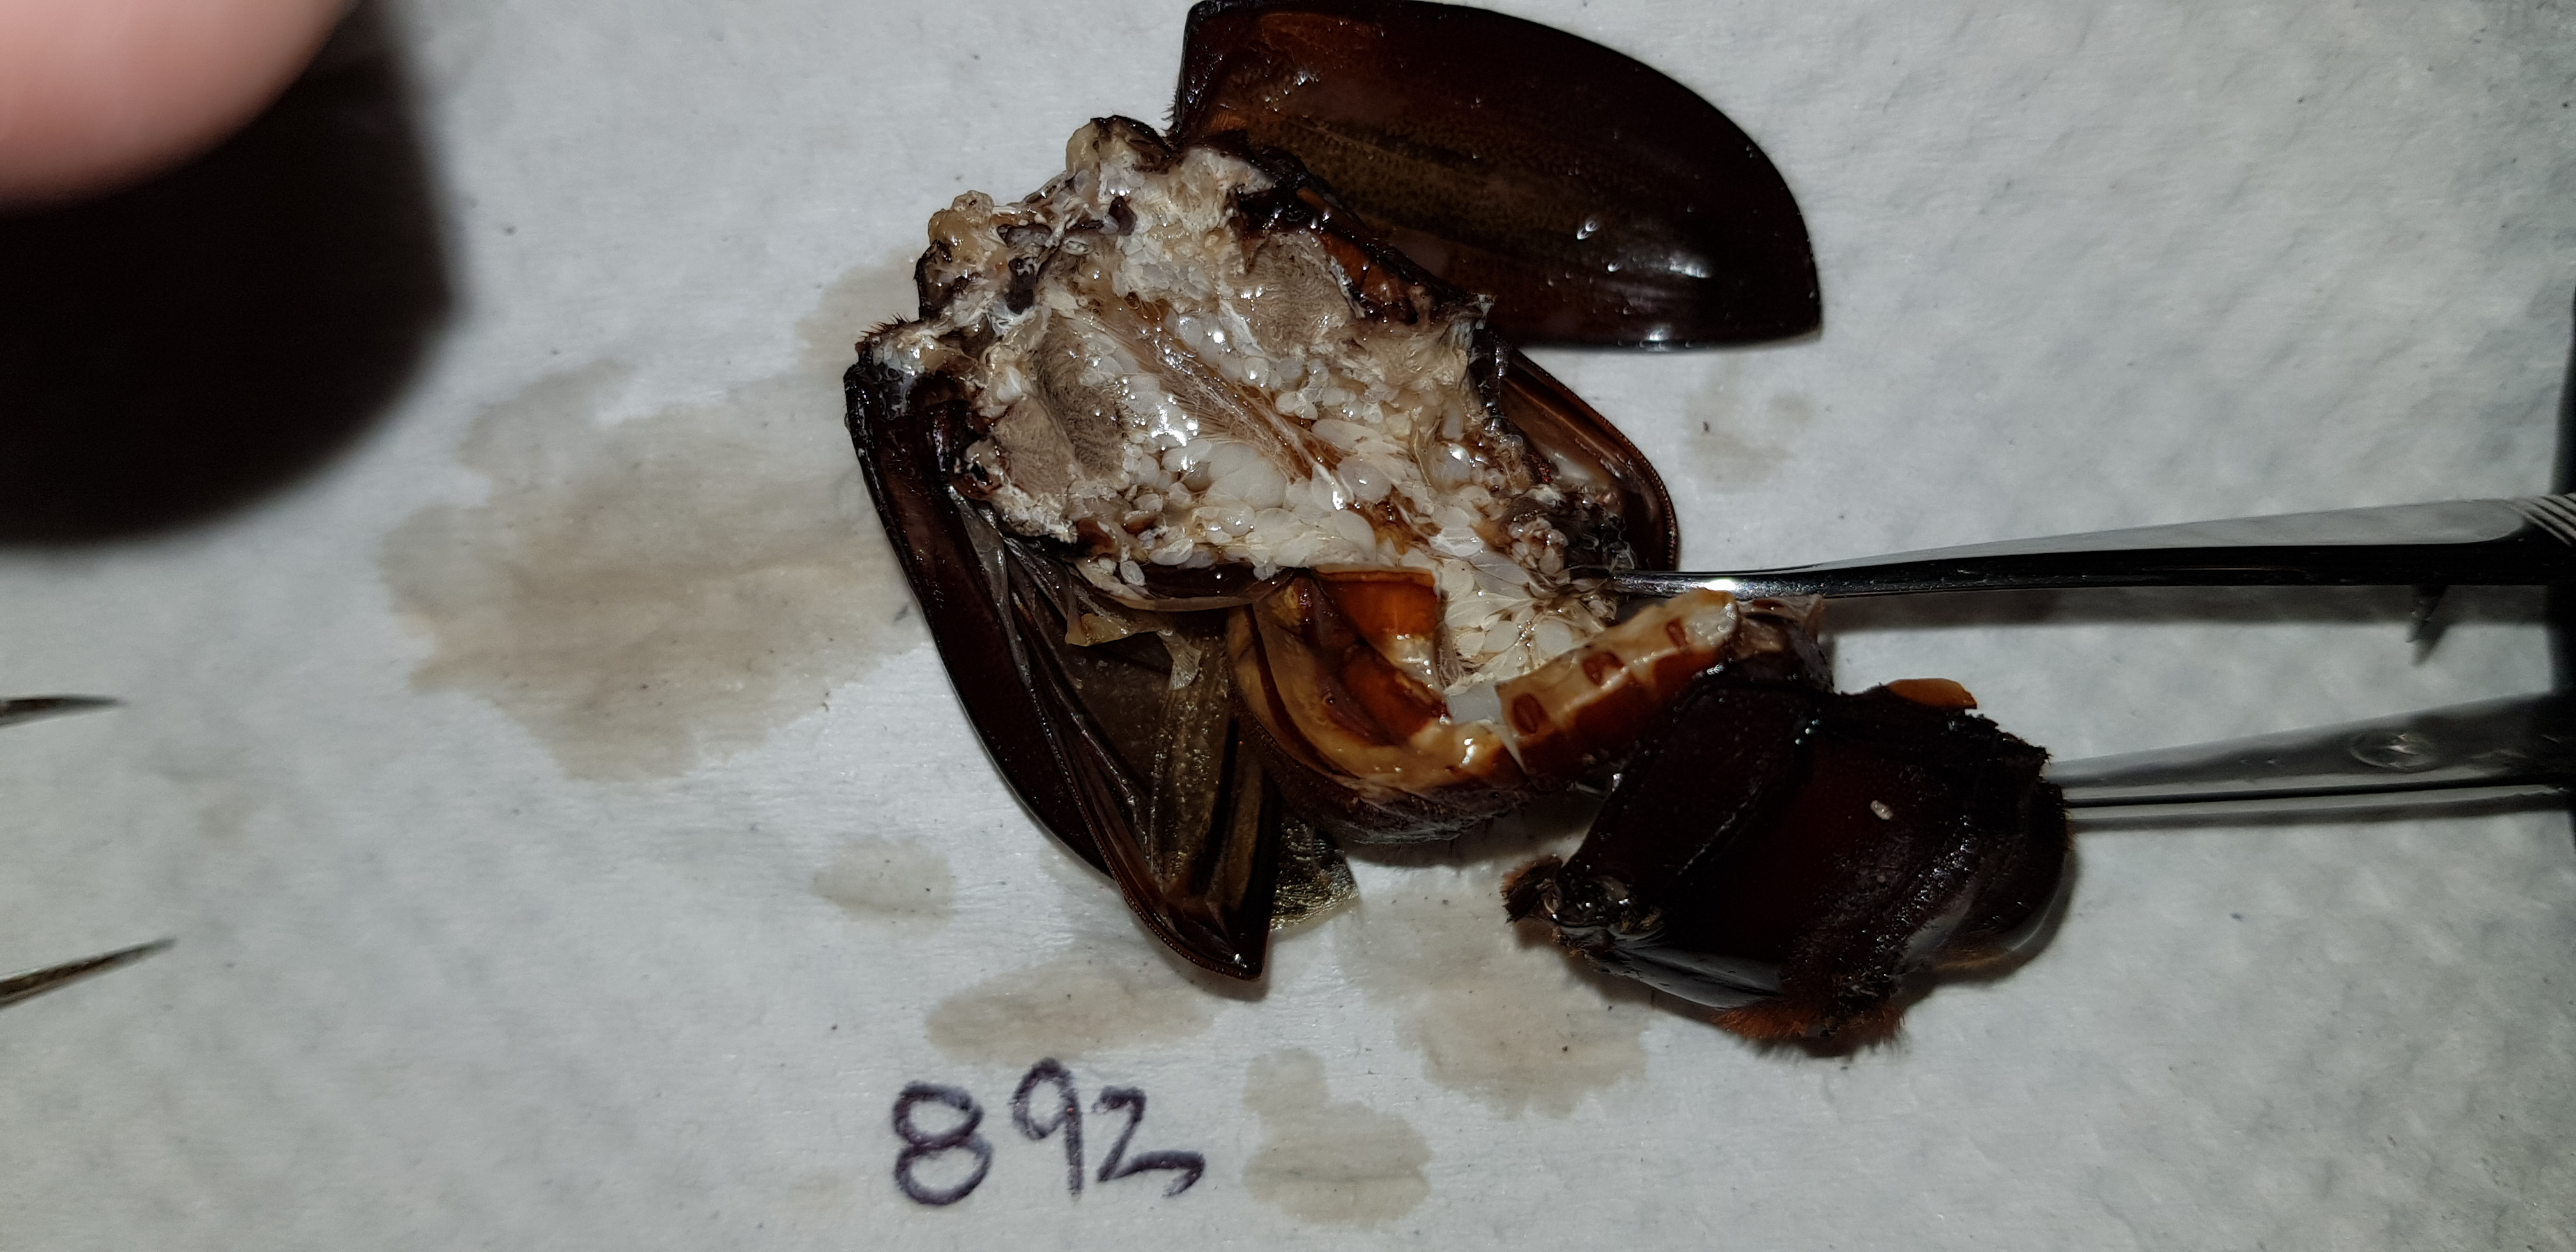
\includegraphics[width=\linewidth, height=\textheight, keepaspectratio]{uploads/btl.pm_image.8d9812a2fc21c8a6.4475673432203839325f5265702d312076697275732e6a7067.jpg}
    \caption{Bioassay: DUG42-1; Treatment: virus; Beetle ID: 57}
\end{figure}
\clearpage

\begin{figure}[h!]
    \centering
    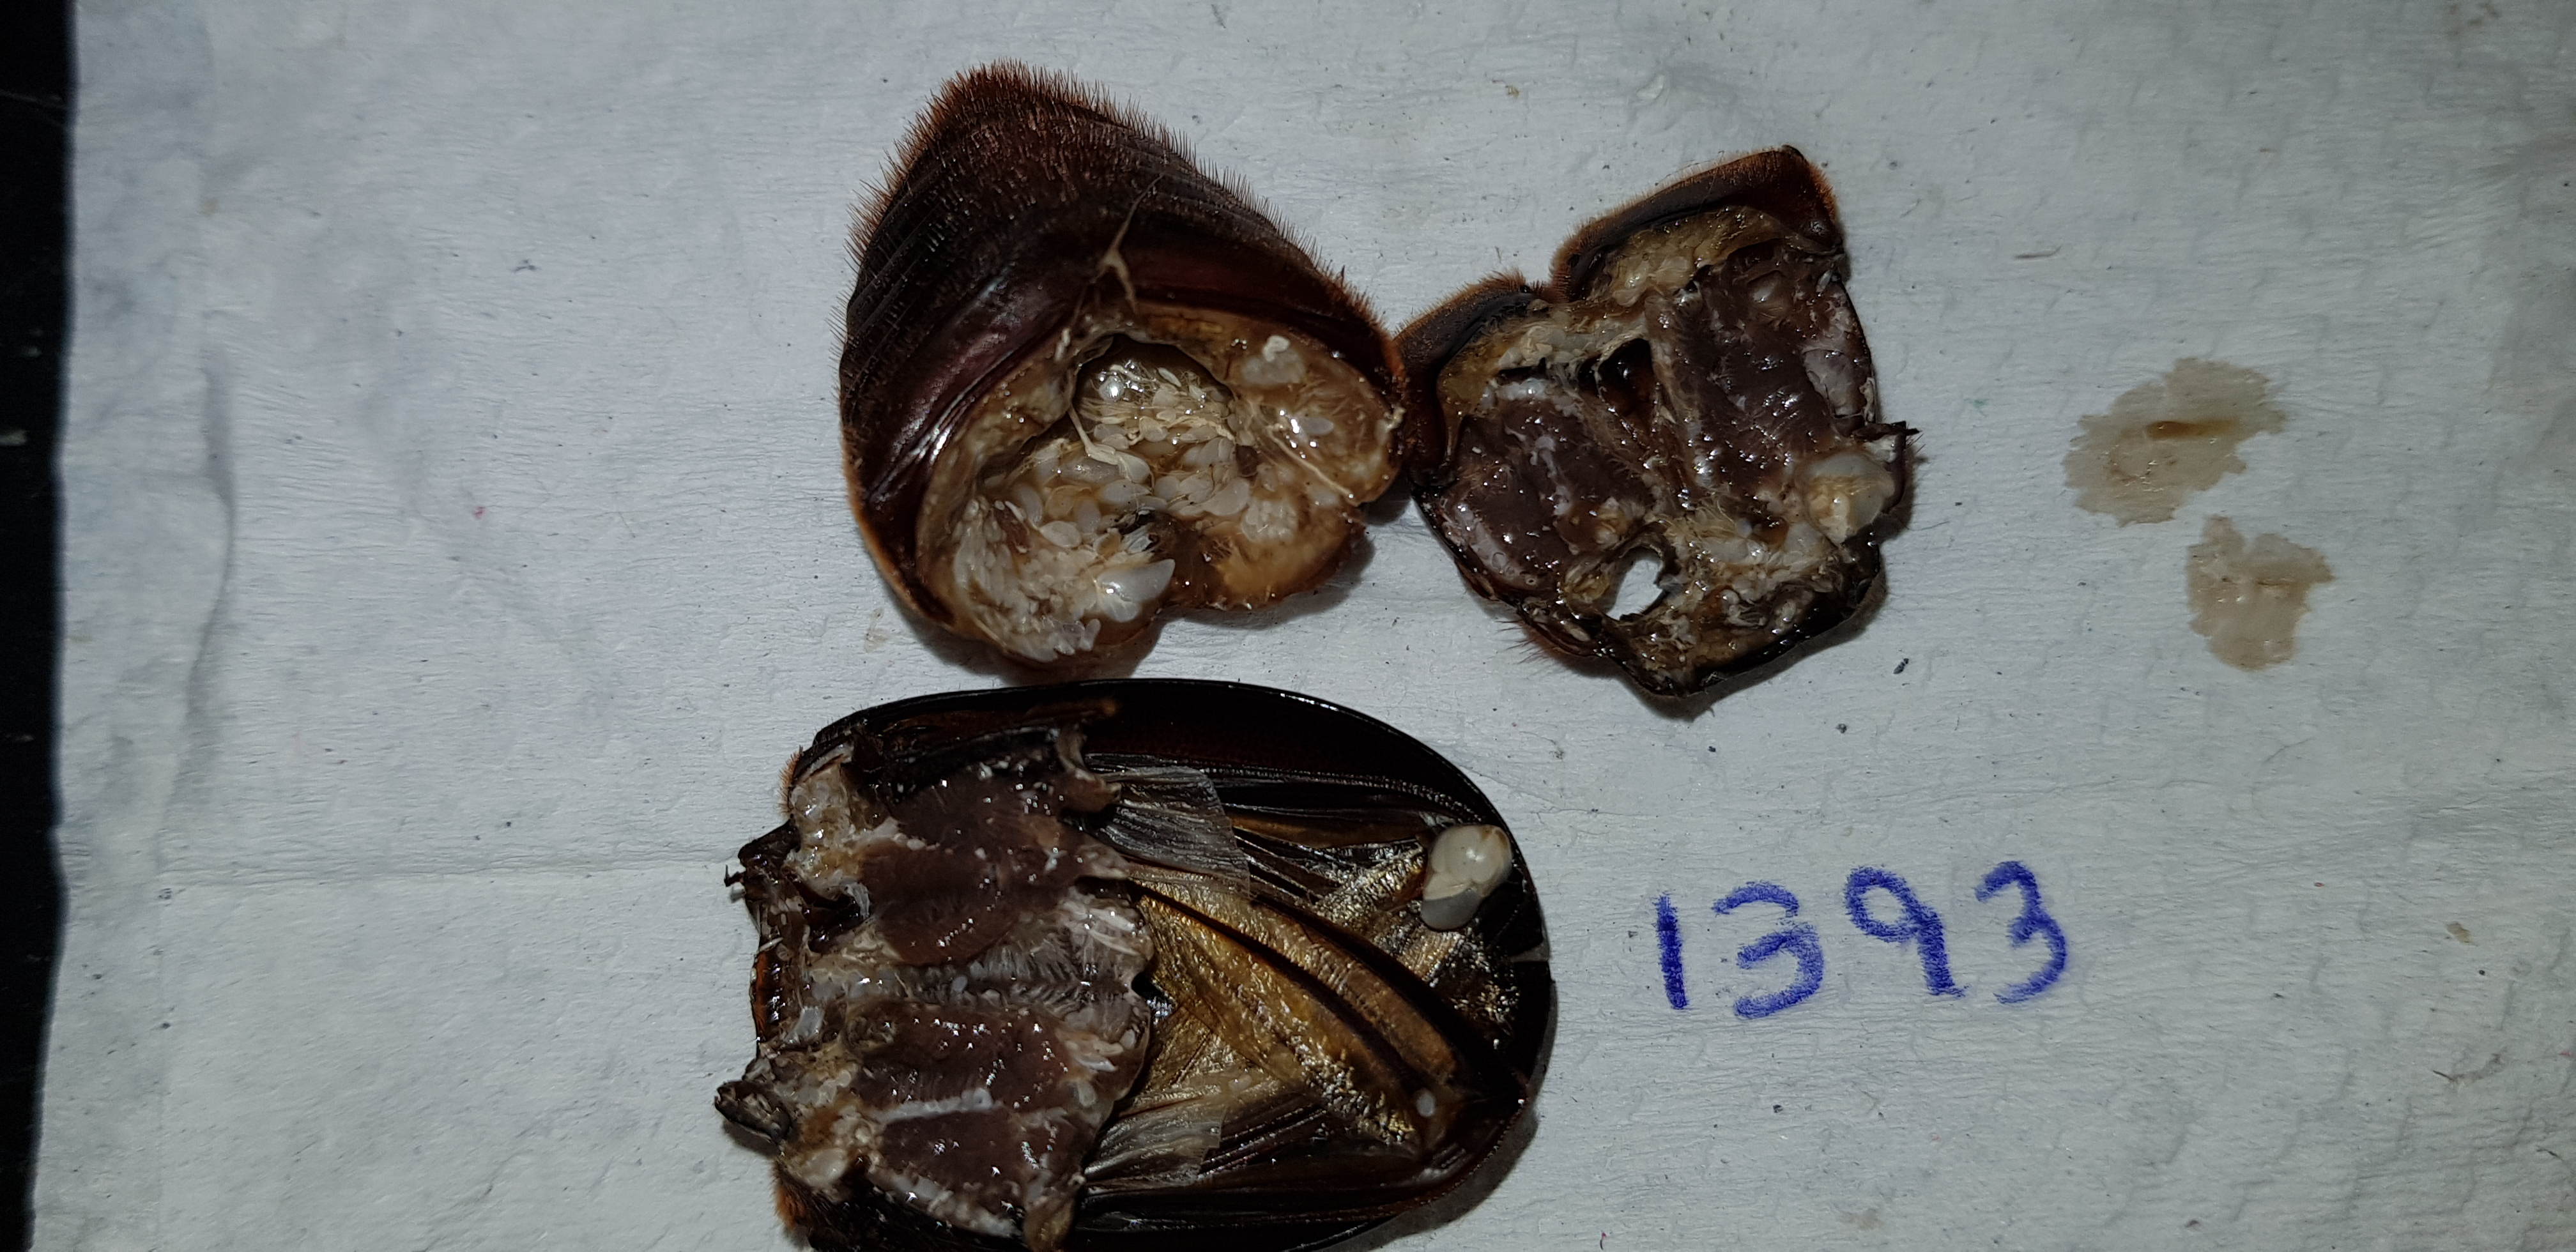
\includegraphics[width=\linewidth, height=\textheight, keepaspectratio]{uploads/btl.pm_image.80a417bc99ec8482.447567343220313339335f5265702d312076697275732e6a7067.jpg}
    \caption{Bioassay: DUG42-1; Treatment: virus; Beetle ID: 58}
\end{figure}
\clearpage

\begin{figure}[h!]
    \centering
    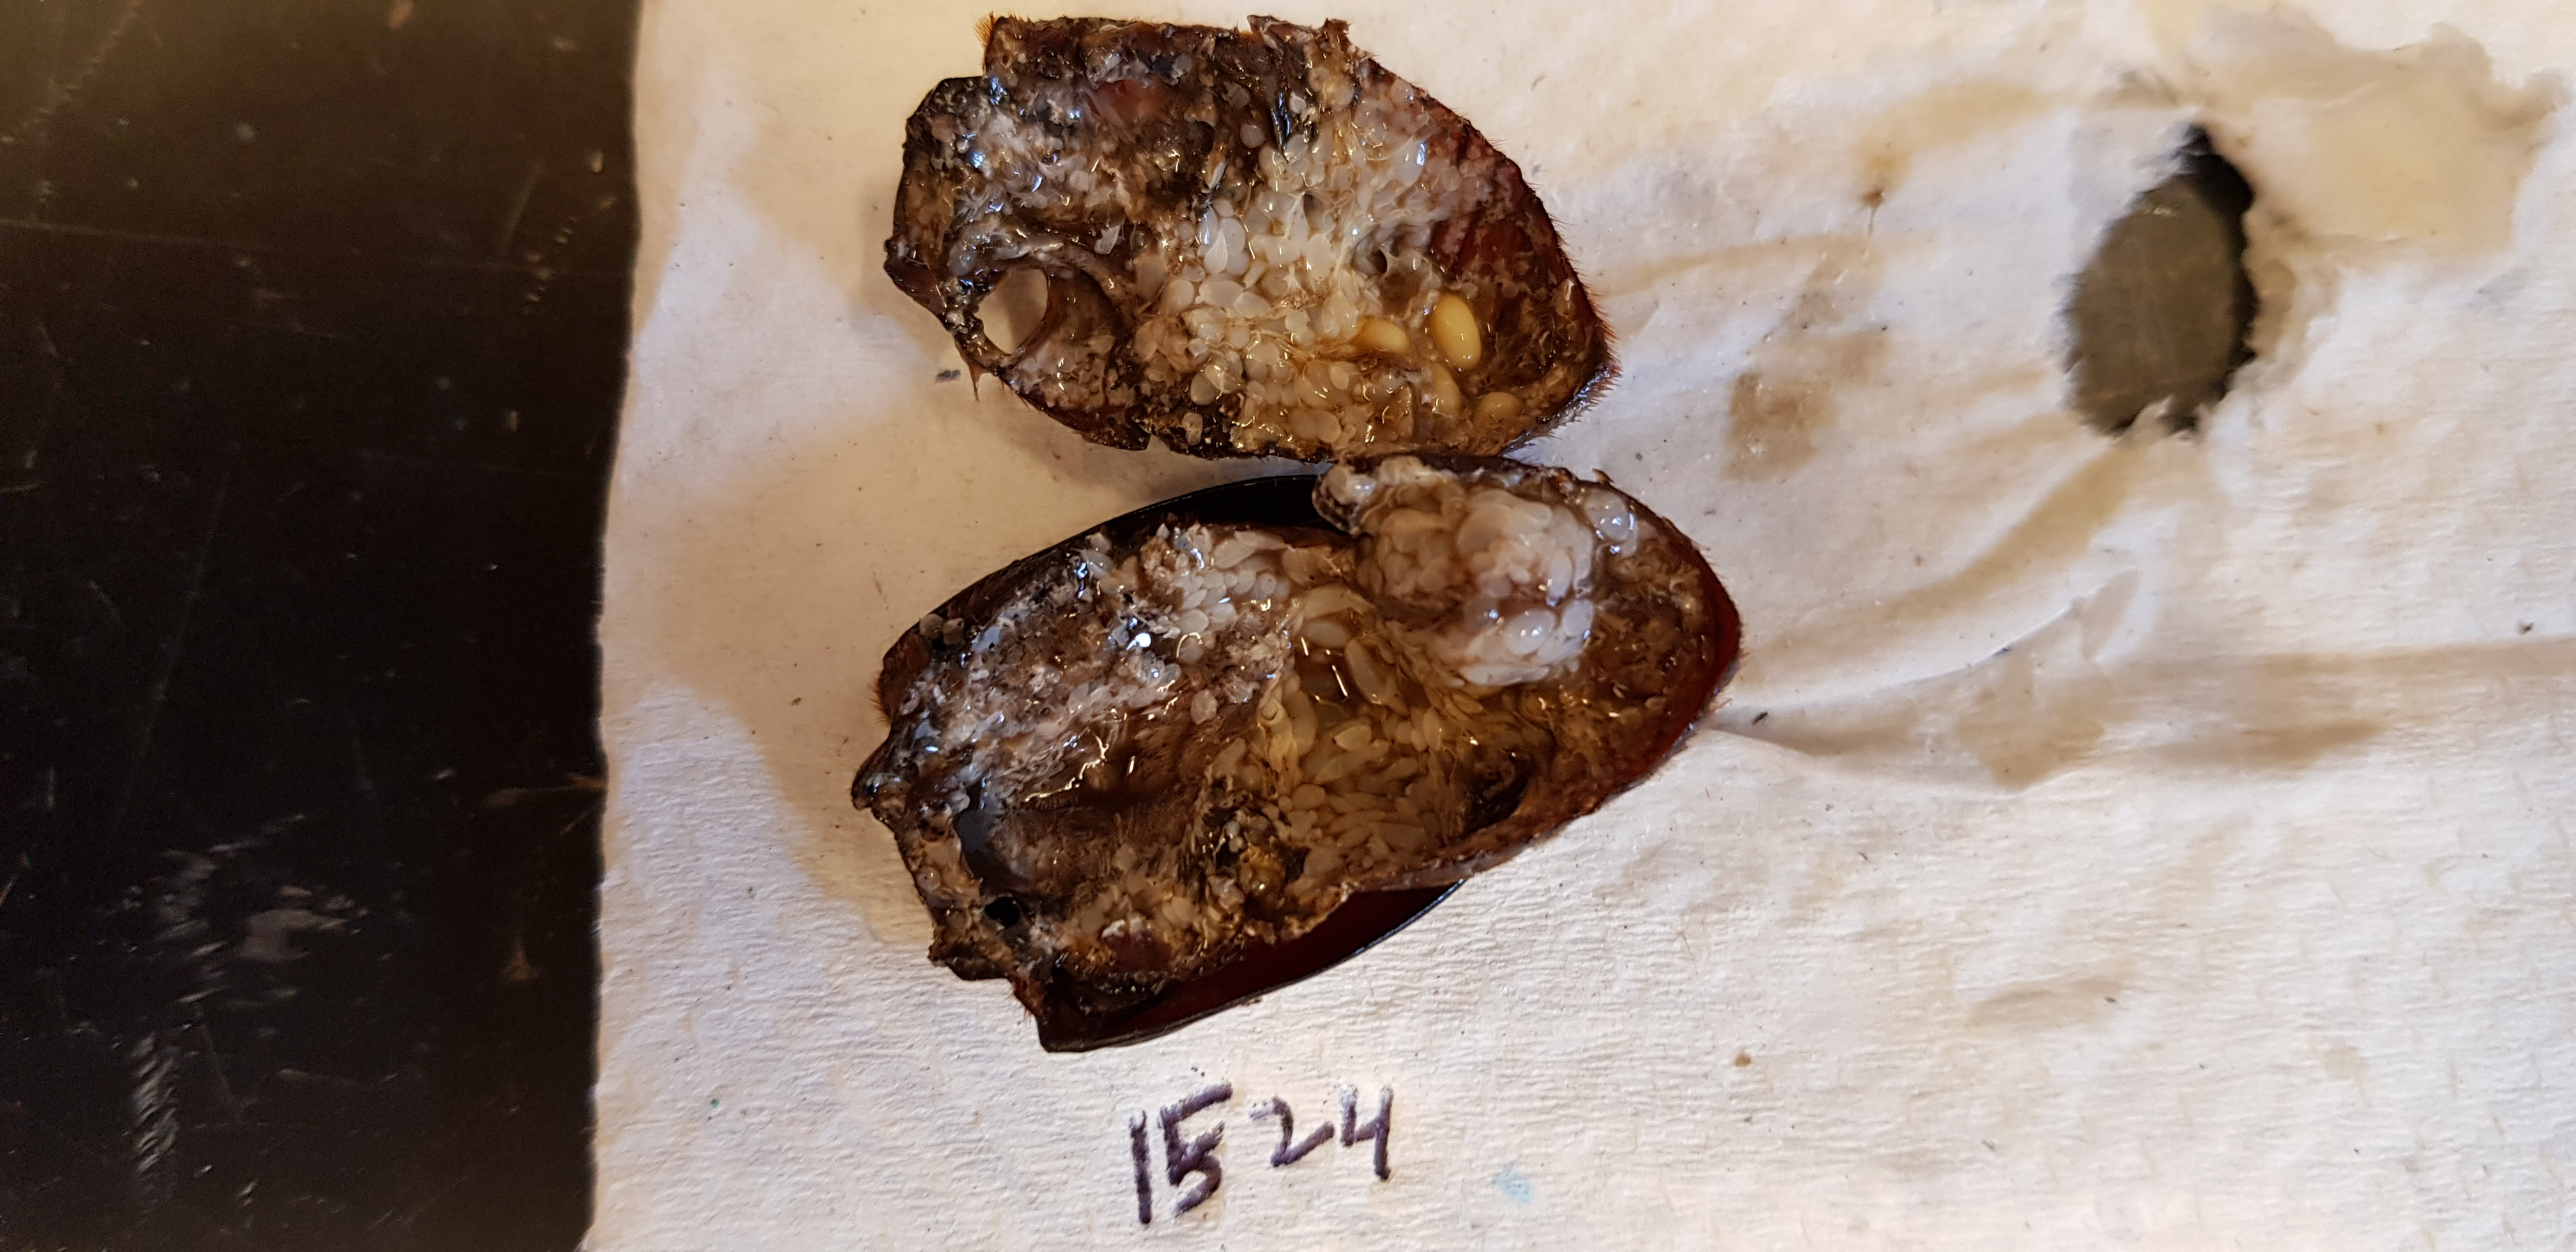
\includegraphics[width=\linewidth, height=\textheight, keepaspectratio]{uploads/btl.pm_image.873c1f3fdf74a9dc.447567343220313532345f5265702d312076697275732e6a7067.jpg}
    \caption{Bioassay: DUG42-1; Treatment: virus; Beetle ID: 59}
\end{figure}
\clearpage

\begin{figure}[h!]
    \centering
    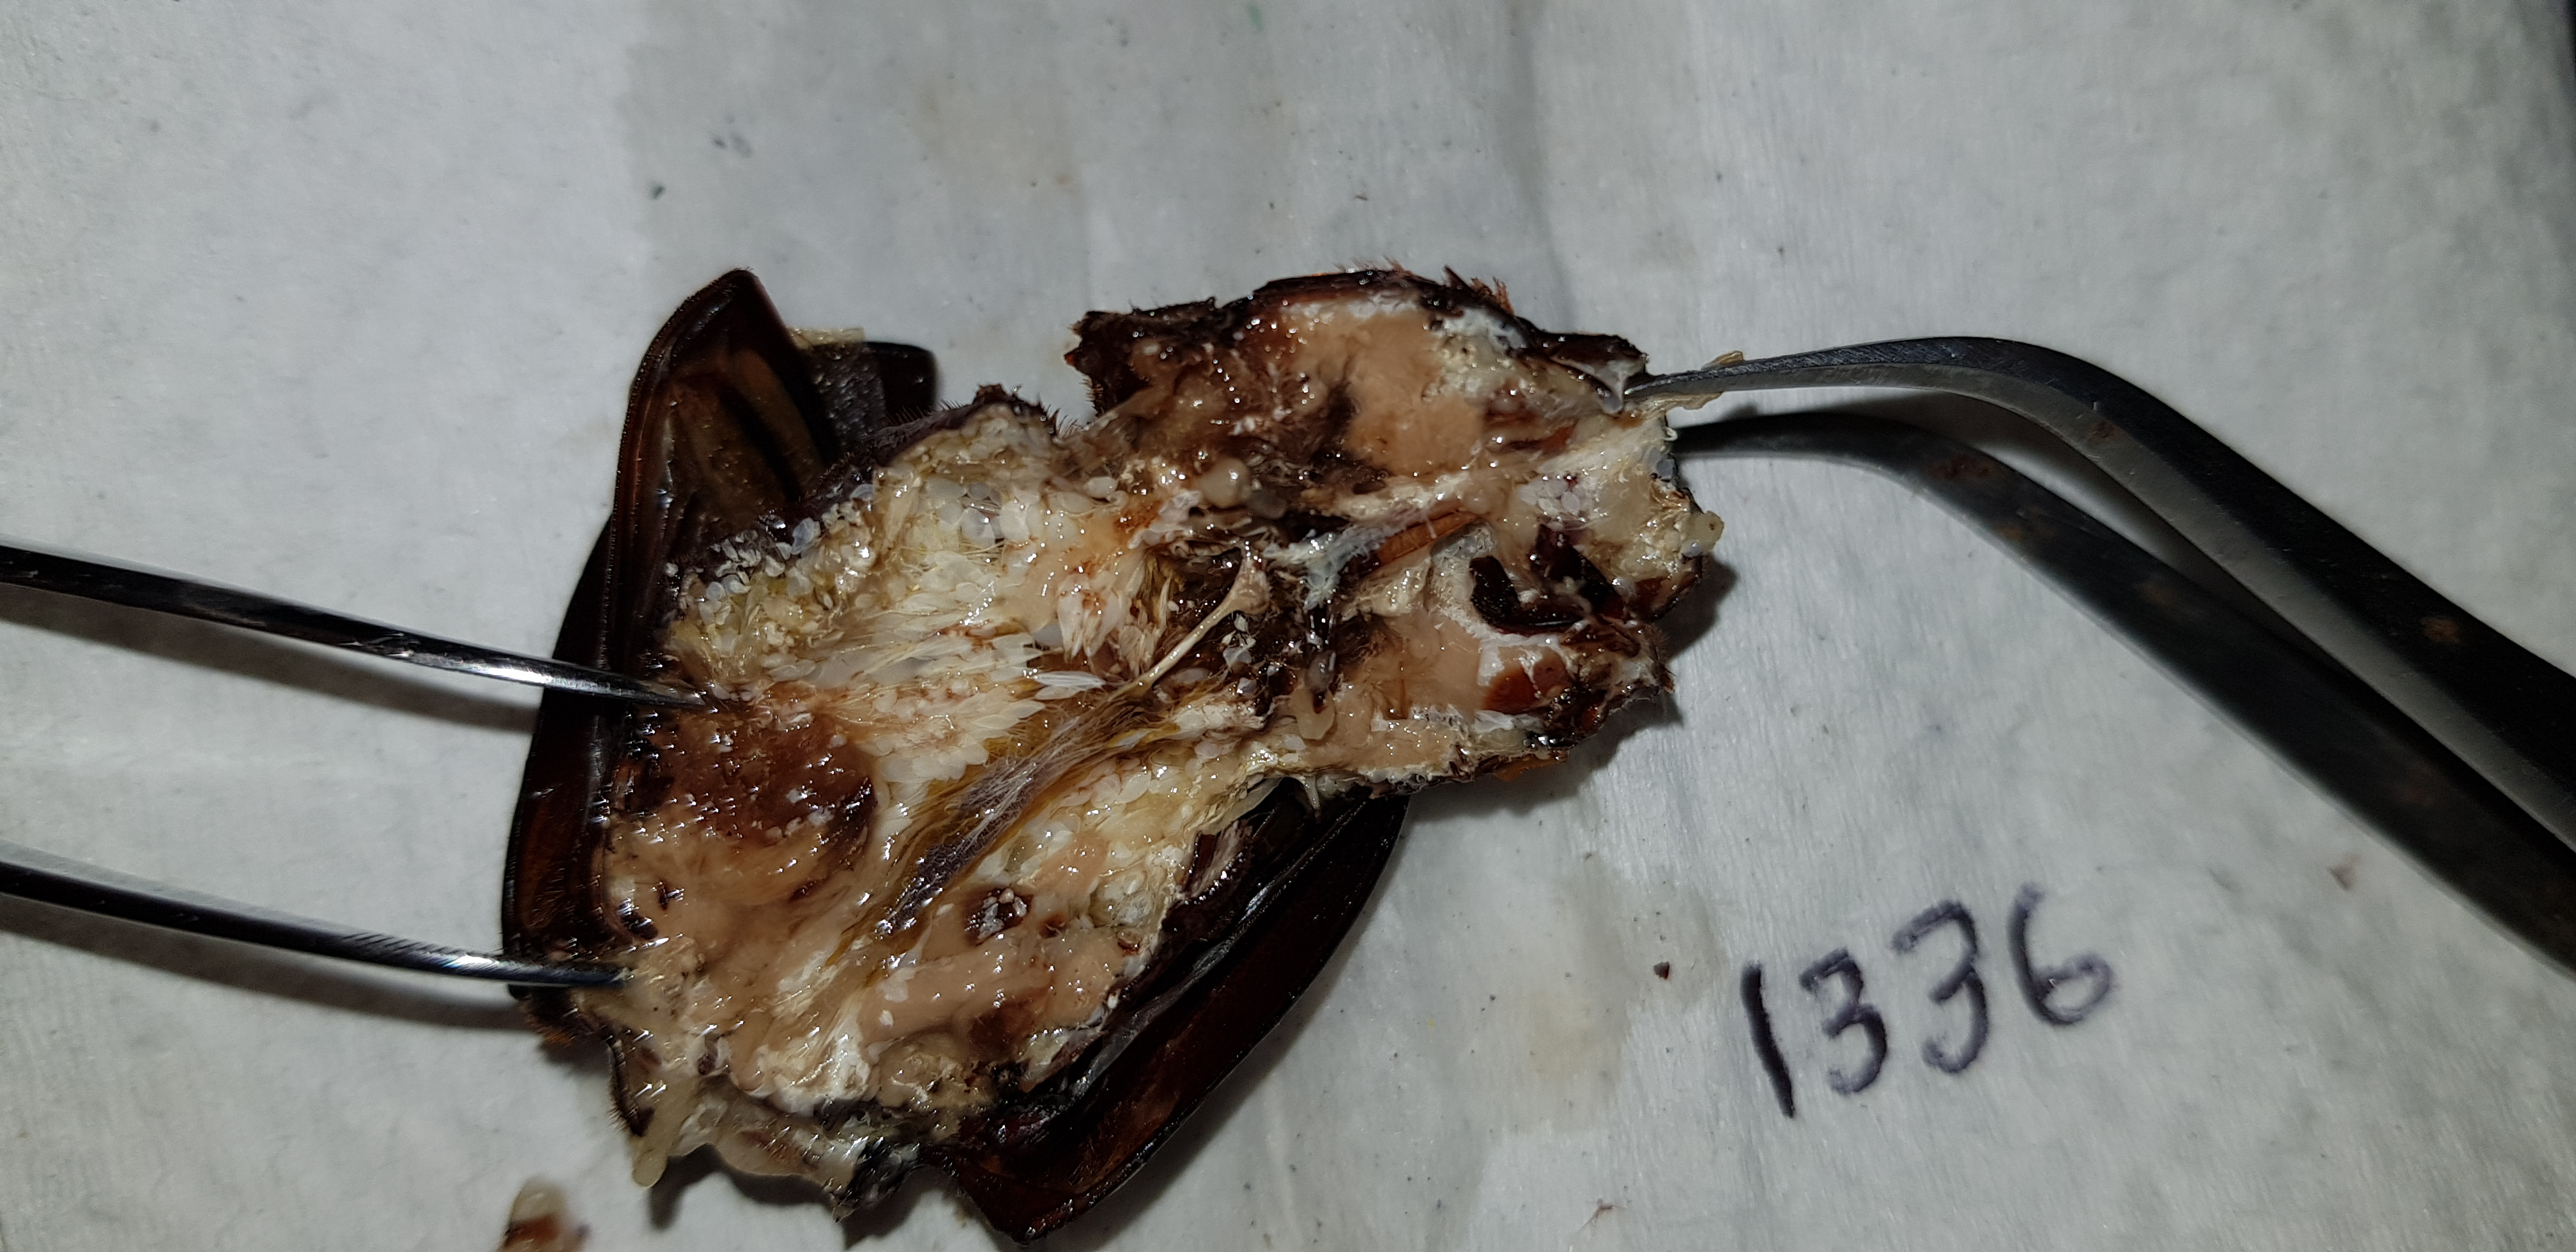
\includegraphics[width=\linewidth, height=\textheight, keepaspectratio]{uploads/btl.pm_image.ad66be521cf7f169.447567343220313333365f5265702d312076697275732e6a7067.jpg}
    \caption{Bioassay: DUG42-1; Treatment: virus; Beetle ID: 60}
\end{figure}
\clearpage

\begin{figure}[h!]
    \centering
    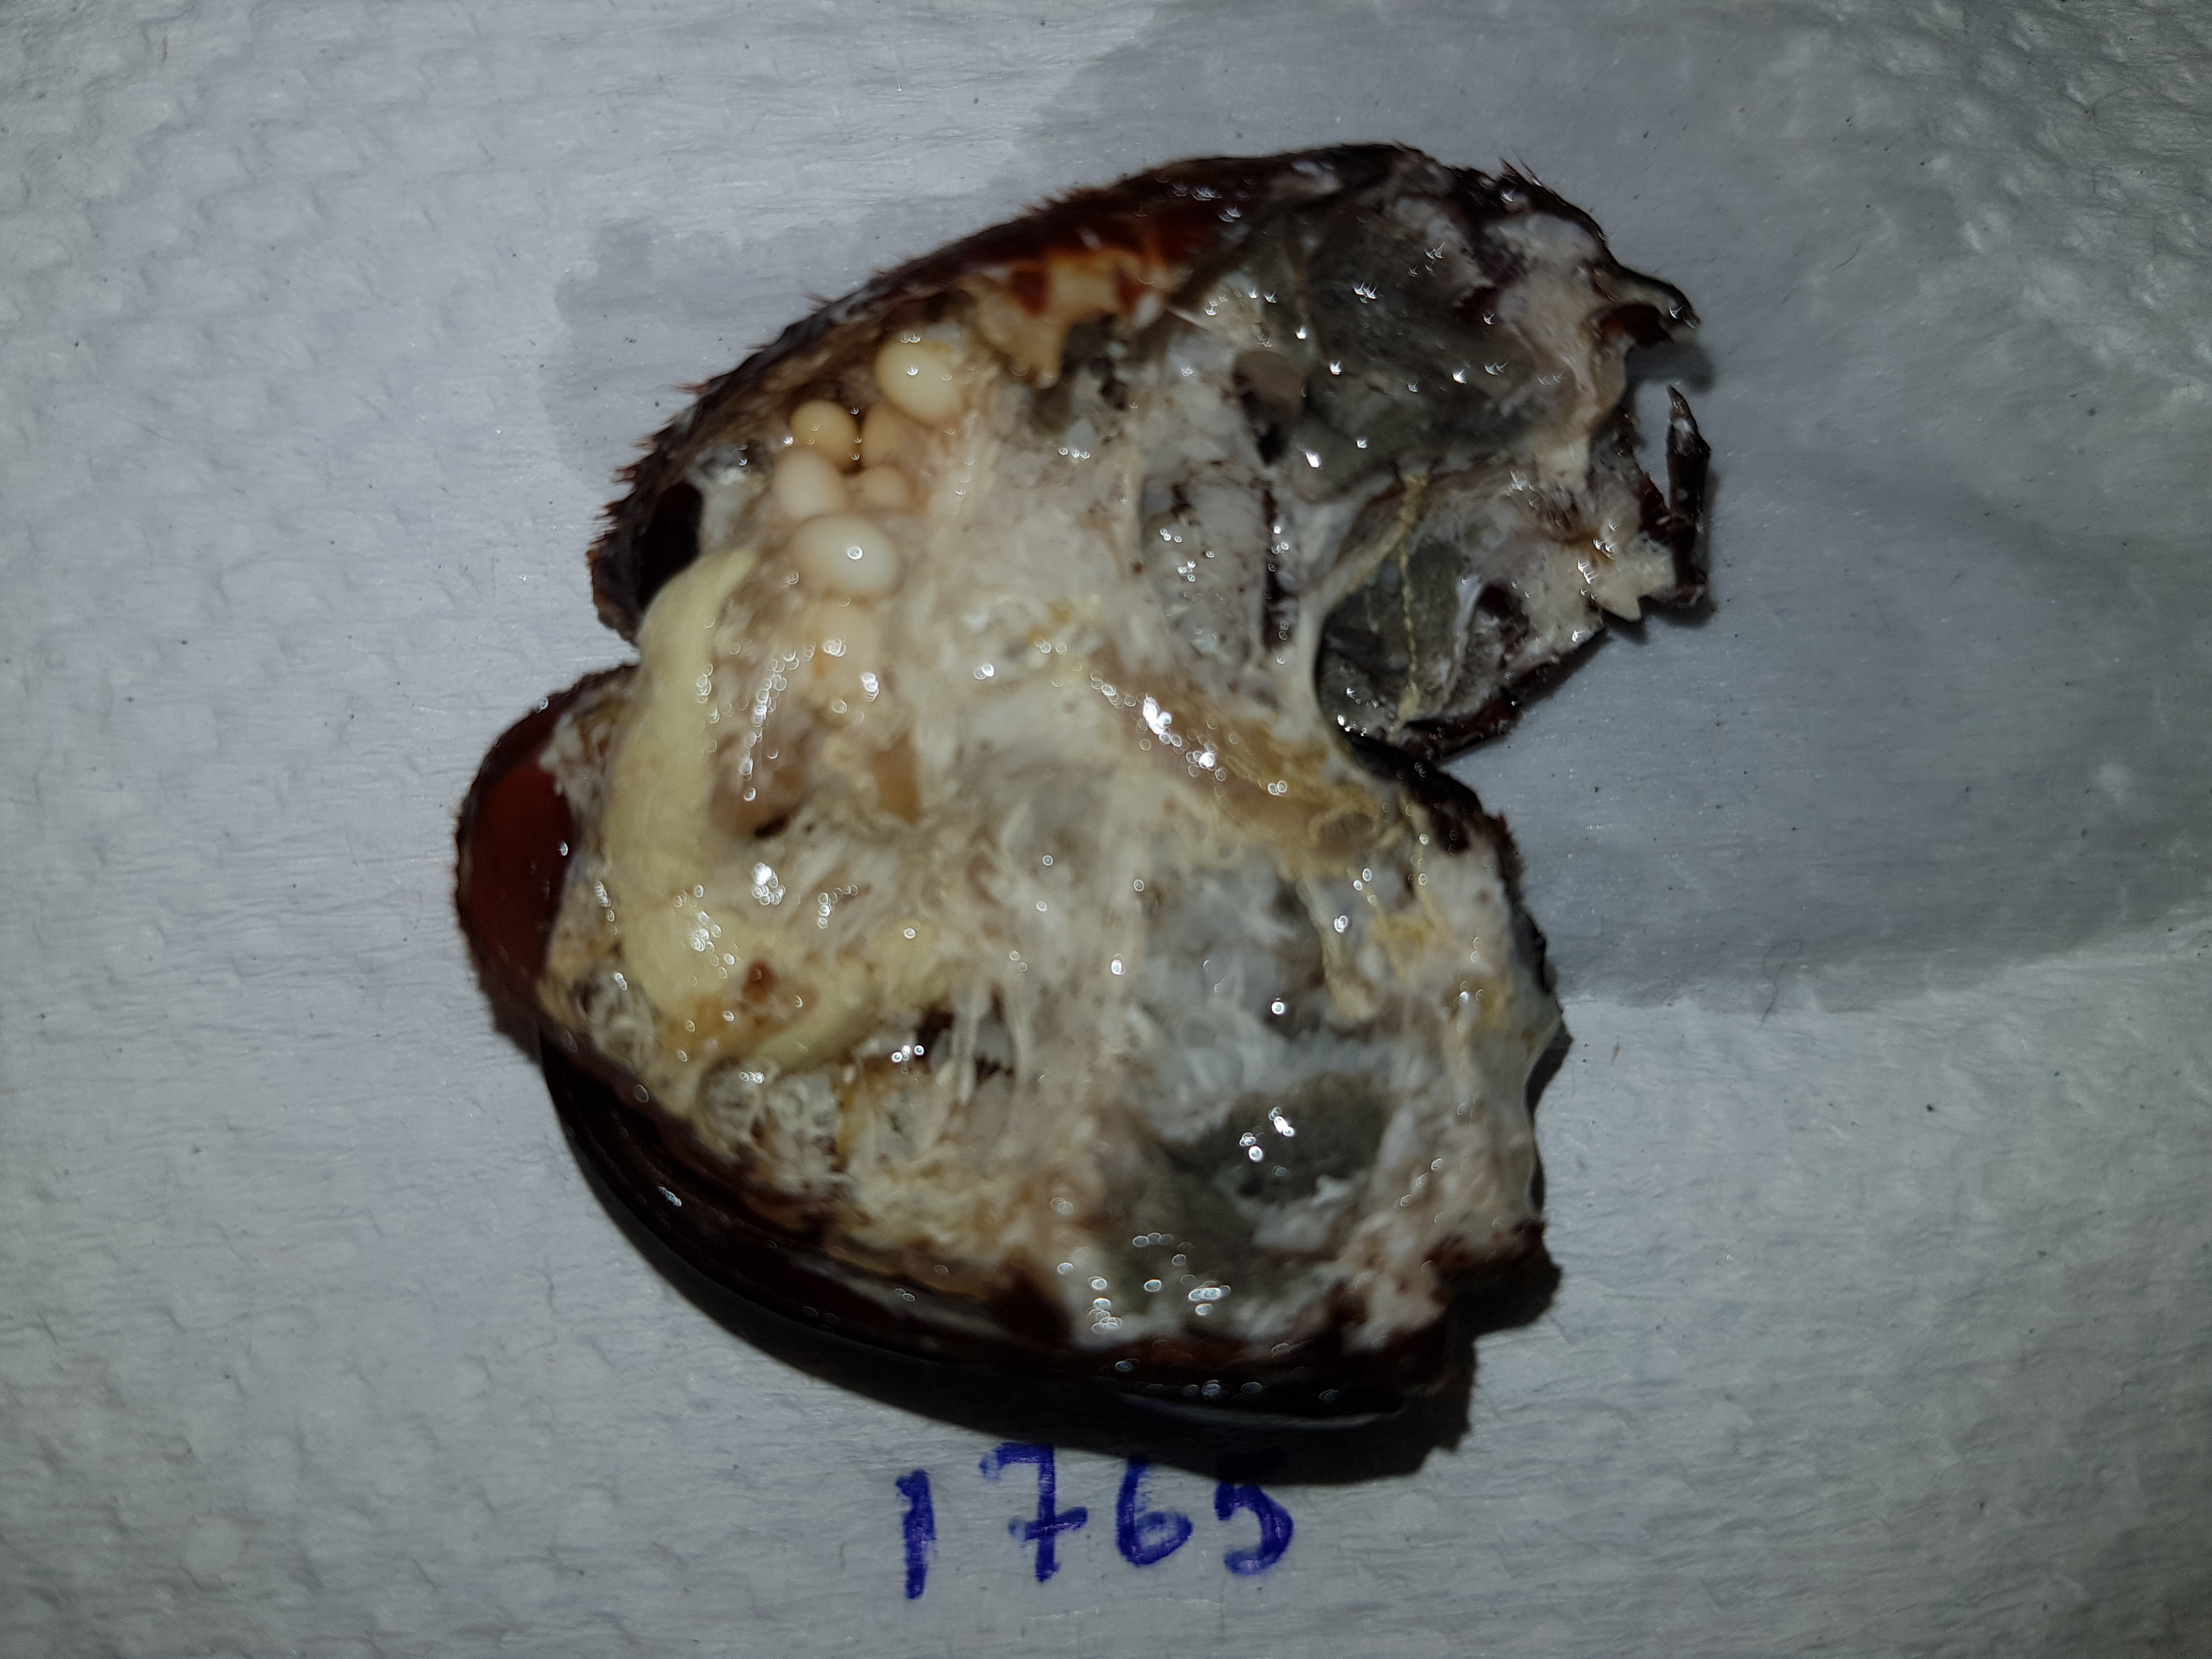
\includegraphics[width=\linewidth, height=\textheight, keepaspectratio]{uploads/btl.pm_image.a72e78cfb1716c7b.447567343220313736355f5265702d322076697275732e6a7067.jpg}
    \caption{Bioassay: DUG42-2; Treatment: virus; Beetle ID: 71}
\end{figure}
\clearpage

\begin{figure}[h!]
    \centering
    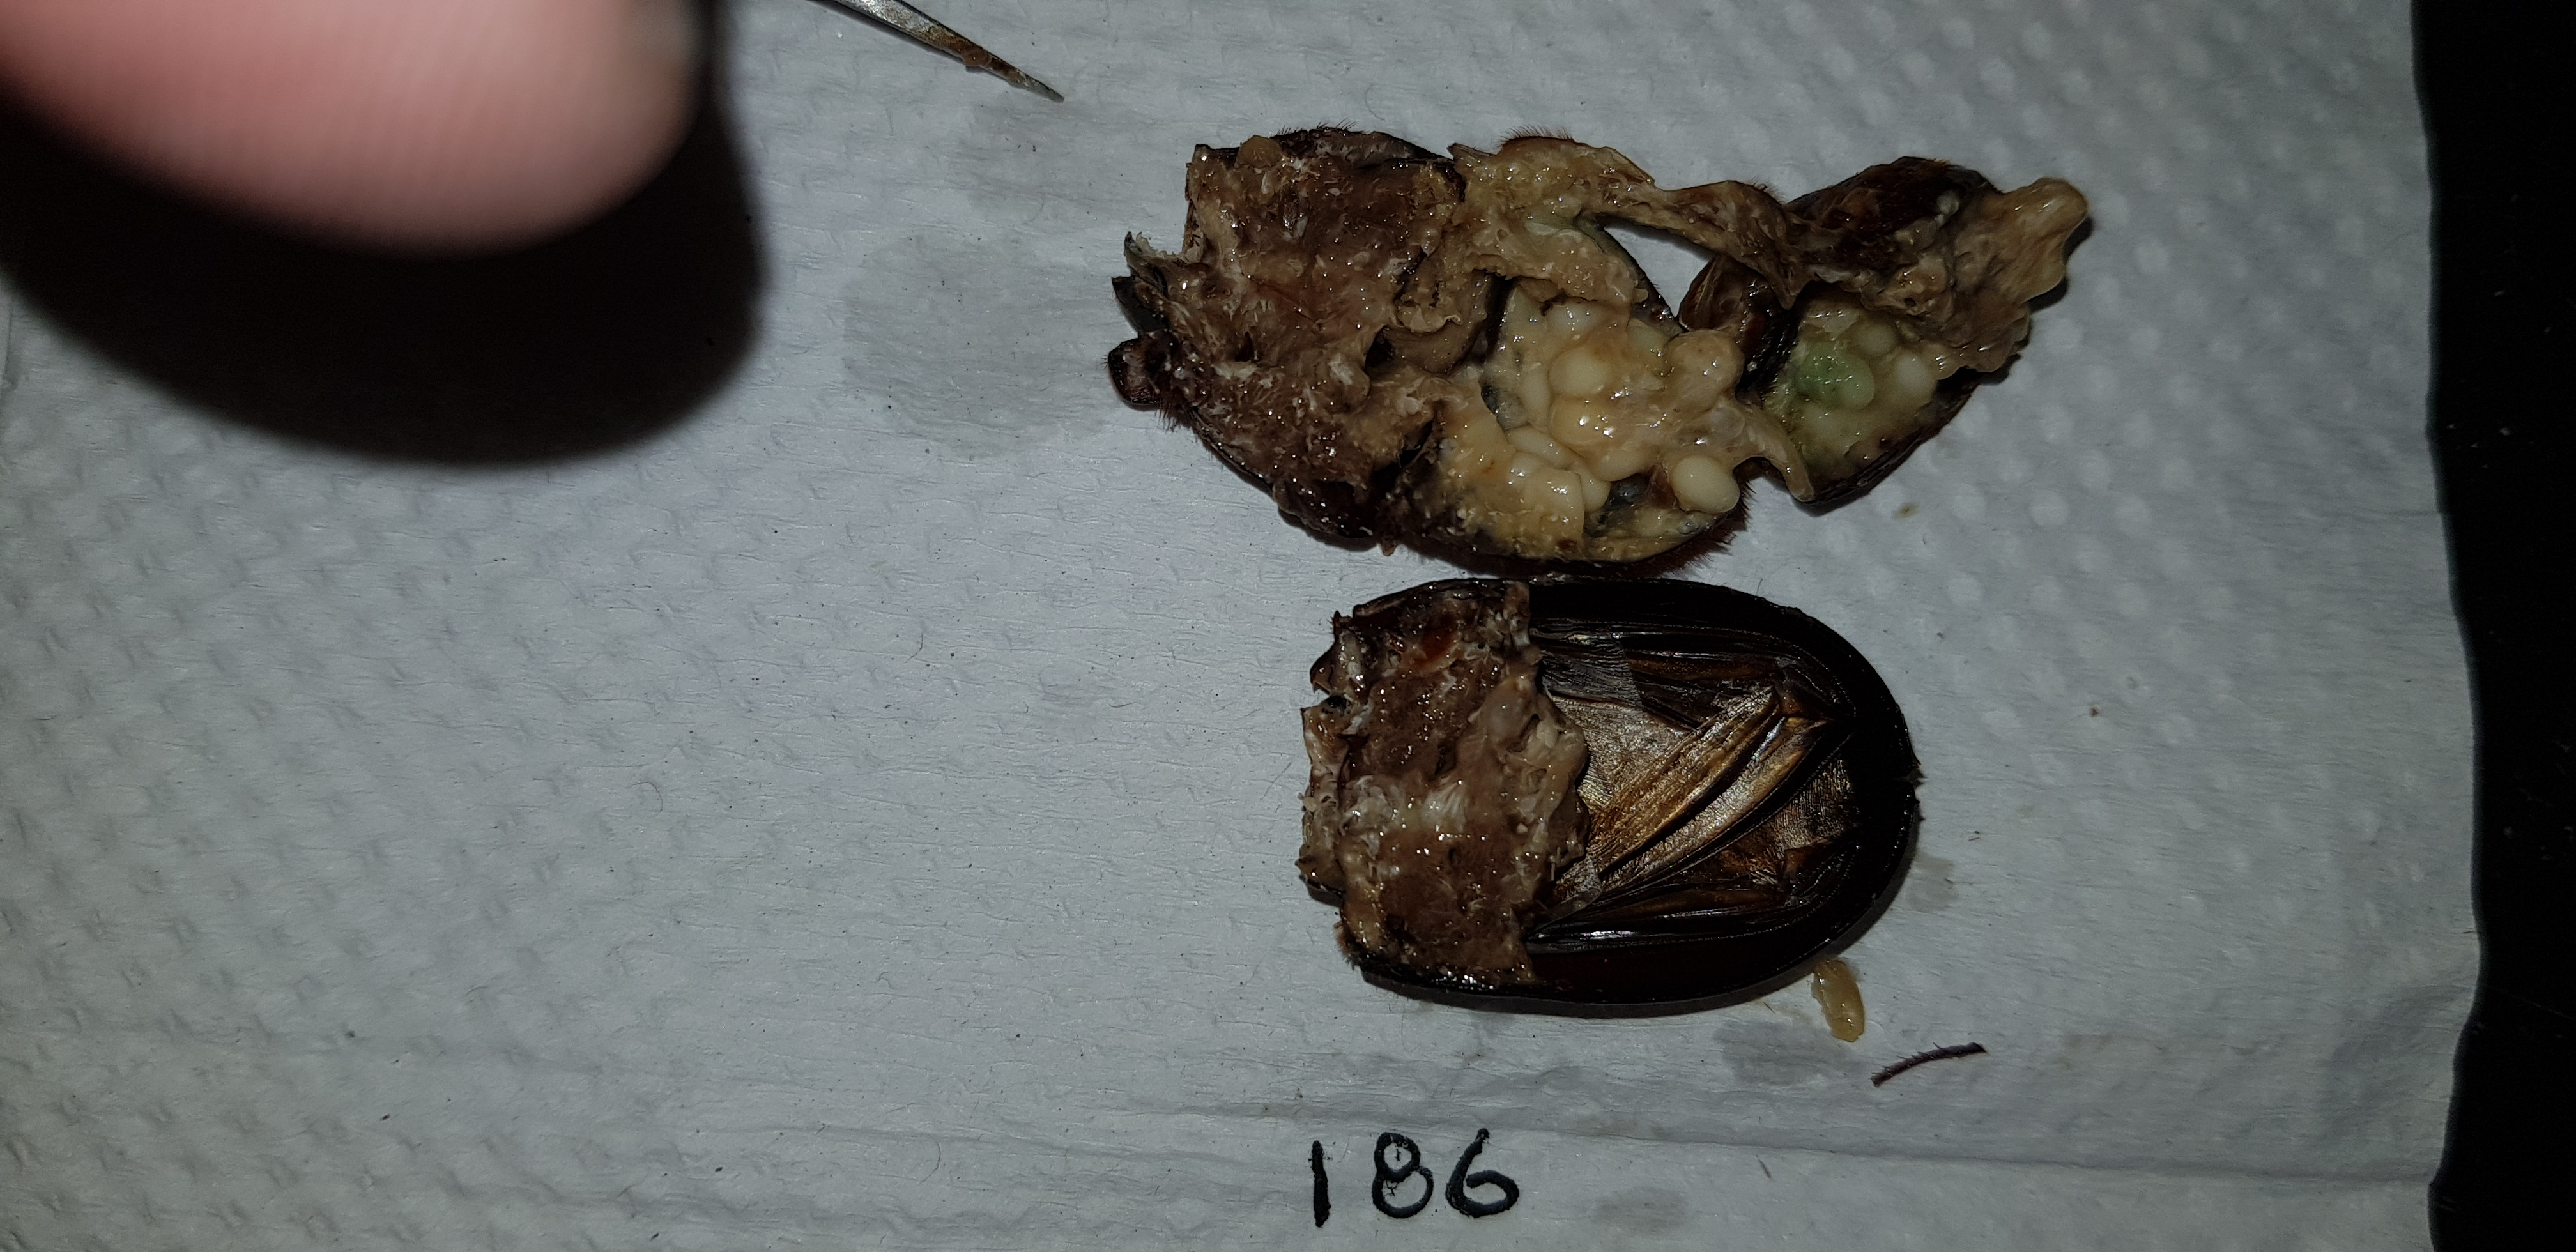
\includegraphics[width=\linewidth, height=\textheight, keepaspectratio]{uploads/btl.pm_image.a2228bddd234a4cb.4475673432203138365f5265702d322076697275732e6a7067.jpg}
    \caption{Bioassay: DUG42-2; Treatment: virus; Beetle ID: 72}
\end{figure}
\clearpage

\begin{figure}[h!]
    \centering
    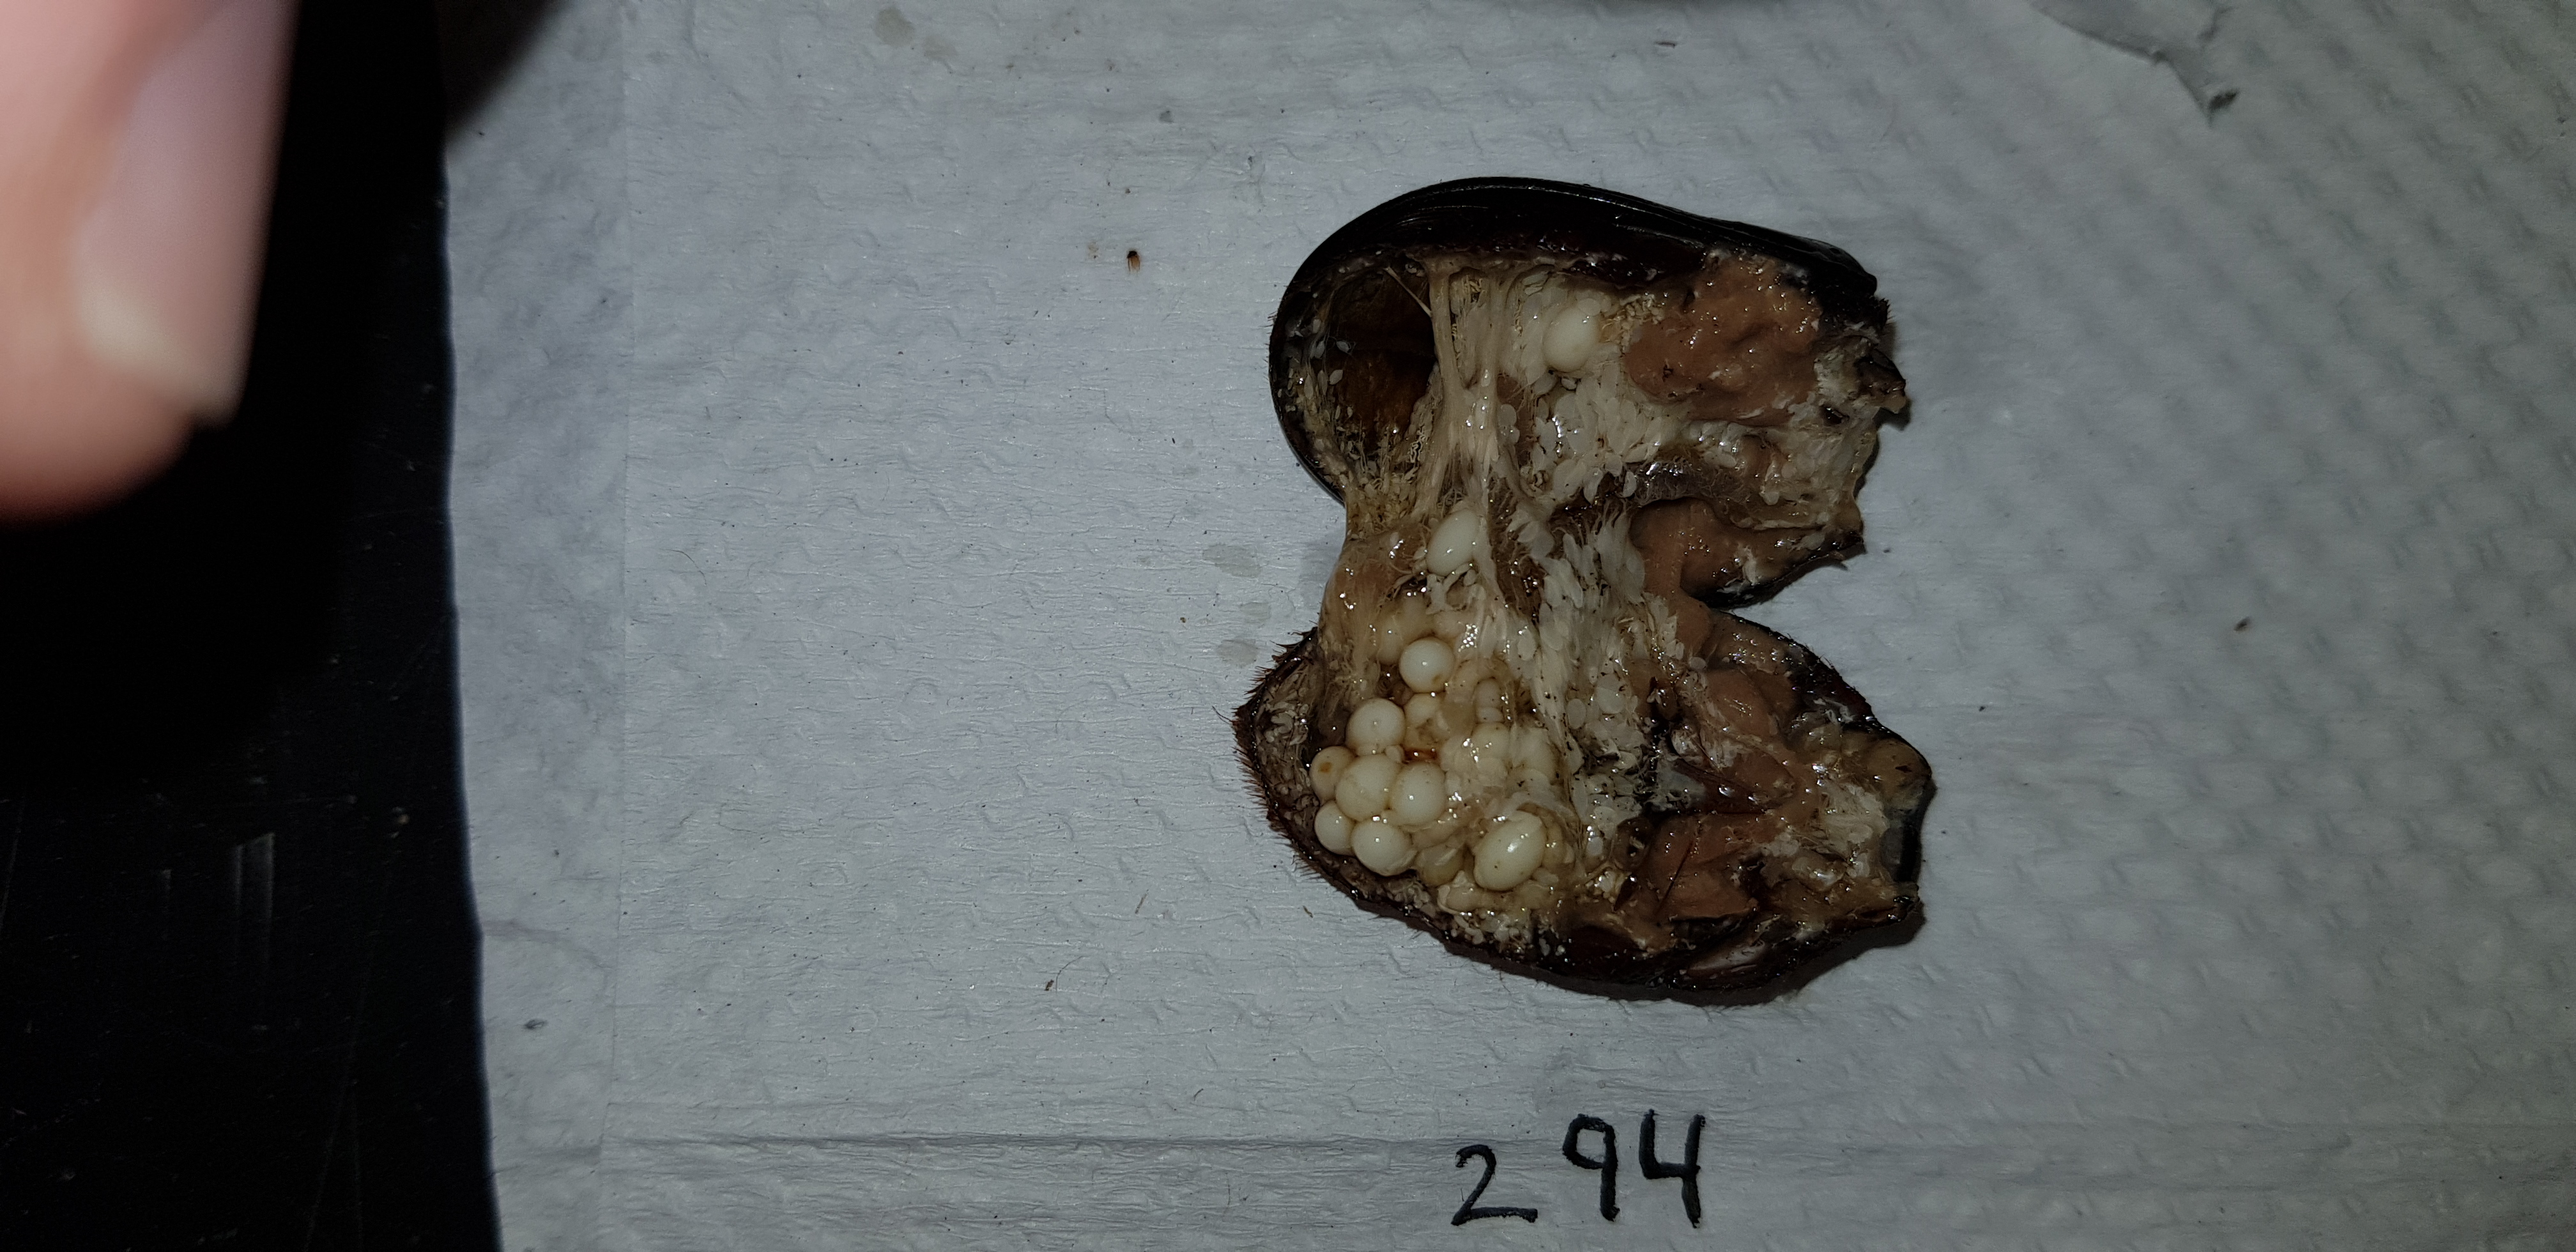
\includegraphics[width=\linewidth, height=\textheight, keepaspectratio]{uploads/btl.pm_image.93628d405386753a.4475673432203239345f7265702d322076697275732e6a7067.jpg}
    \caption{Bioassay: DUG42-2; Treatment: virus; Beetle ID: 73}
\end{figure}
\clearpage

\begin{figure}[h!]
    \centering
    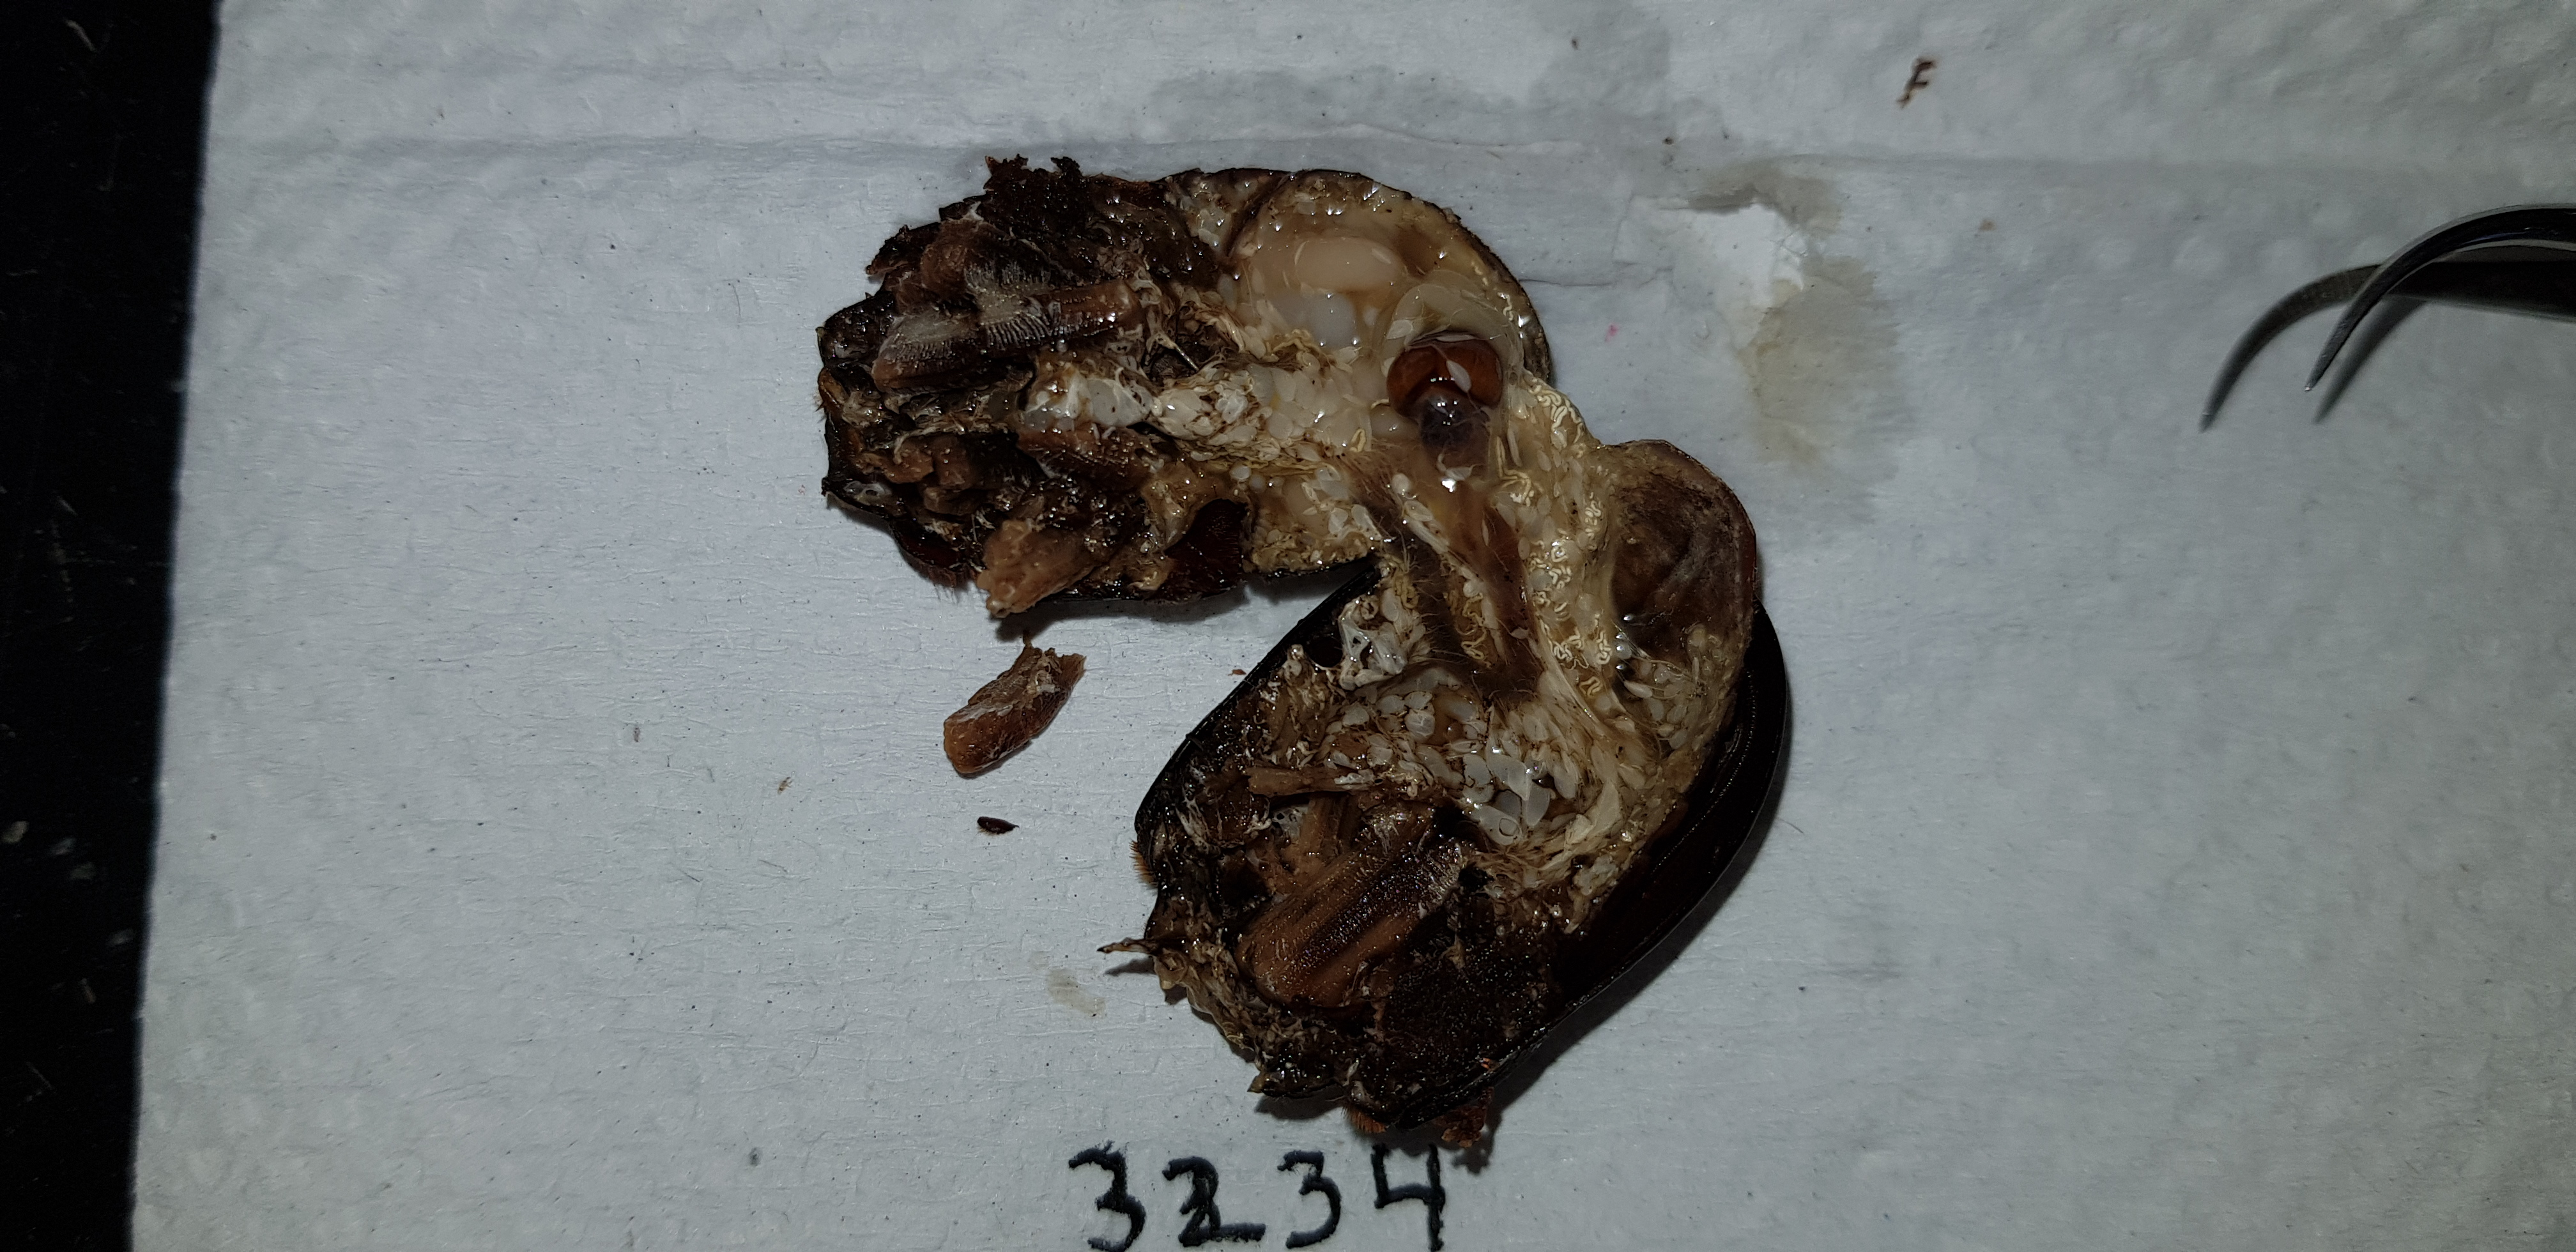
\includegraphics[width=\linewidth, height=\textheight, keepaspectratio]{uploads/btl.pm_image.b38f50ea460c96da.447567343220333233345f5265702d322076697275732e6a7067.jpg}
    \caption{Bioassay: DUG42-2; Treatment: virus; Beetle ID: 74}
\end{figure}
\clearpage

\begin{figure}[h!]
    \centering
    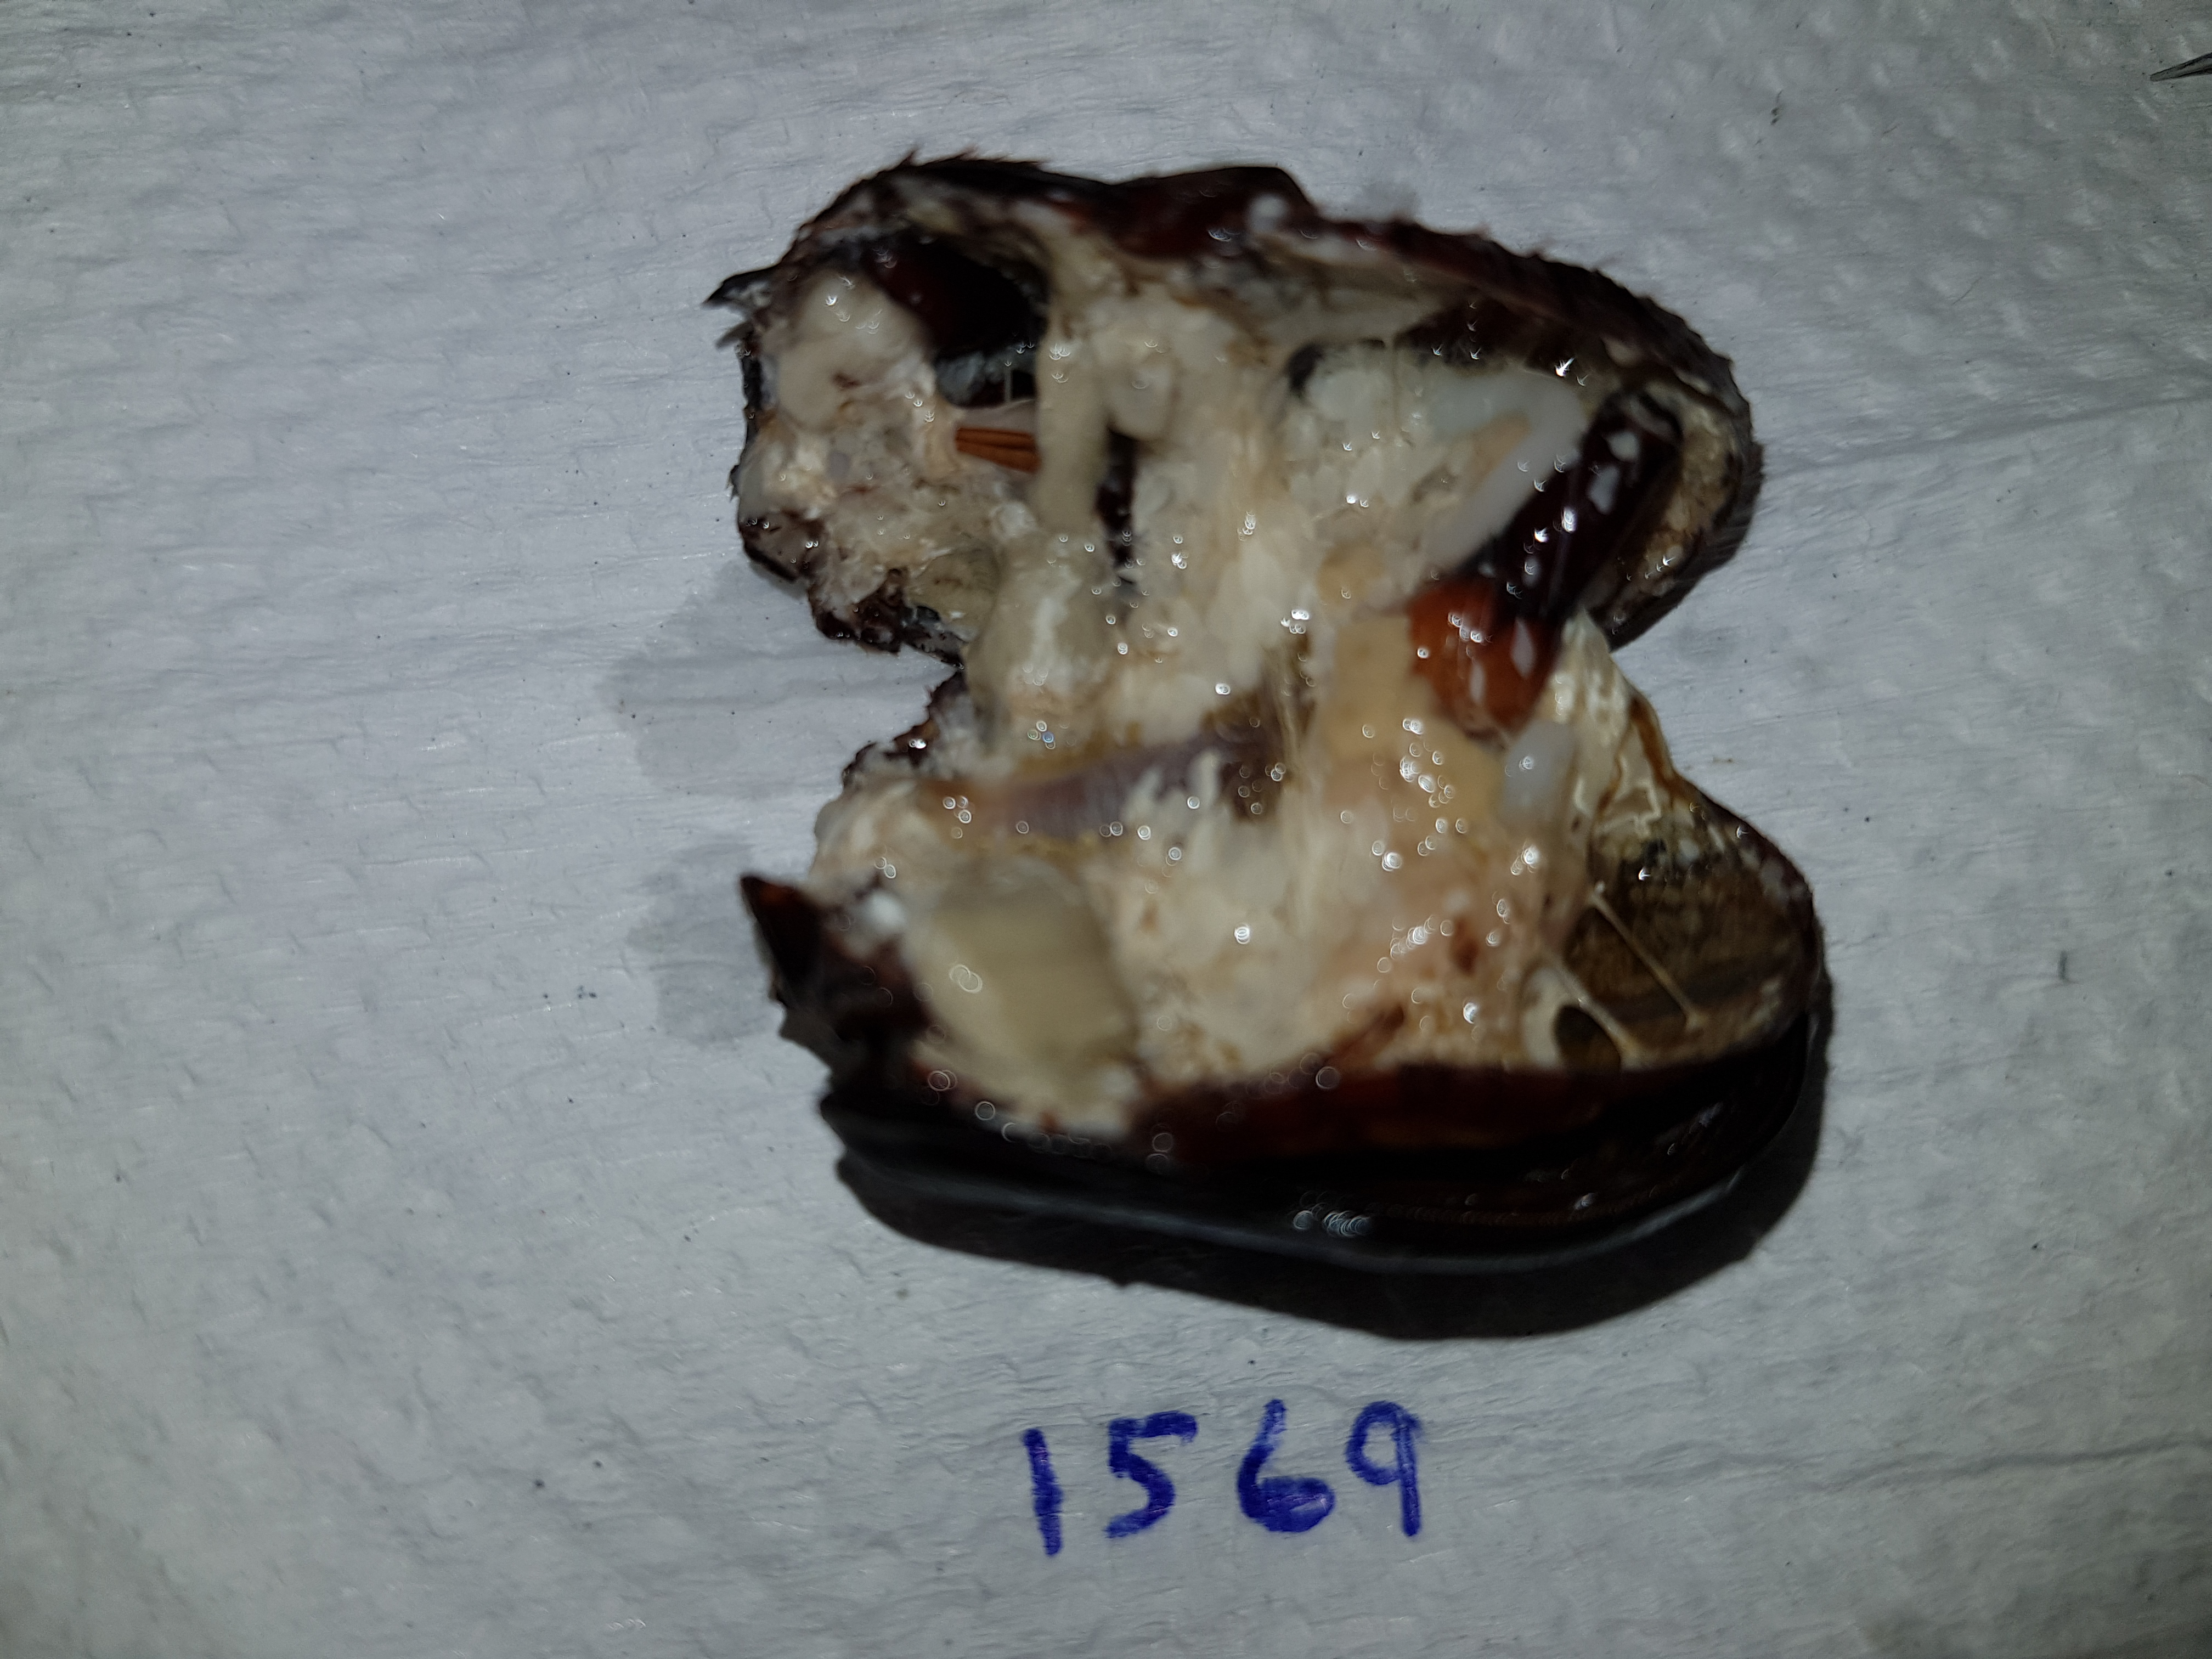
\includegraphics[width=\linewidth, height=\textheight, keepaspectratio]{uploads/btl.pm_image.90077d26c55c5b23.447567343220313536395f5265702d32202076697275732e6a7067.jpg}
    \caption{Bioassay: DUG42-2; Treatment: virus; Beetle ID: 75}
\end{figure}
\clearpage


\end{document}